\RequirePackage[l2tabu,orthodox]{nag} % Раскомментировав, можно в логе получать рекомендации относительно правильного использования пакетов и предупреждения об устаревших и нерекомендуемых пакетах
% Формат А4, 14pt (ГОСТ Р 7.0.11-2011, 5.3.6)
\documentclass[a4paper,14pt]{extreport}

\input{common/packages}  % Пакеты общие для диссертации и автореферата
\input{Dissertation/dispackages}         % Пакеты для диссертации
\input{Dissertation/userpackages}        % Пакеты для специфических пользовательских задач

\input{Dissertation/setup}               % Упрощённые настройки шаблона

\input{Dissertation/preamblenames}       % Переопределение именований, чтобы можно было и в преамбуле использовать
\input{common/newnames}  % Новые переменные, которые могут использоваться во всём проекте

%%% Основные сведения %%%
\newcommand{\thesisAuthor}             % Диссертация, ФИО автора
{%
    \texorpdfstring{% \texorpdfstring takes two arguments and uses the first for (La)TeX and the second for pdf
        Карапетян Сергей Артурович% так будет отображаться на титульном листе или в тексте, где будет использоваться переменная
    }{%
        Карапетян Сергей Артурович% эта запись для свойств pdf-файла. В таком виде, если pdf будет обработан программами для сбора библиографических сведений, будет правильно представлена фамилия.
    }%
}
\newcommand{\thesisUdk}                % Диссертация, УДК
{\todo{xxx.xxx}}
\newcommand{\thesisTitle}              % Диссертация, название
{\texorpdfstring{\MakeUppercase{Влияние рассеяния носителей на шероховатой поверхности на кинетические и оптические процессы в размерно-квантованных системах}}{Влияние шероховатой поверхности на кинетические явления во внешних полях}}
\newcommand{\thesisSpecialtyNumber}    % Диссертация, специальность, номер
{\texorpdfstring{01.04.10}{01.04.10}}
\newcommand{\thesisSpecialtyTitle}     % Диссертация, специальность, название
{\texorpdfstring{Физика полупроводников}{Физика полупроводников}}
\newcommand{\thesisDegree}             % Диссертация, научная степень
{кандидата физико-математических наук}
\newcommand{\thesisCity}               % Диссертация, город защиты
{Тирасполь}
\newcommand{\thesisYear}               % Диссертация, год защиты
{2017}
\newcommand{\thesisOrganization}       % Диссертация, организация
{Приднестровский Государственный Университет им.~Т.Г.~Шевченко}

\newcommand{\thesisInOrganization}       % Диссертация, организация в предложном падеже: Работа выполнена в ...
{Приднестровского Государственного Университета им.~Т.Г.~Шевченко}

\newcommand{\supervisorFio}            % Научный руководитель, ФИО
{Синявский Элерланж Петрович}
\newcommand{\supervisorRegalia}        % Научный руководитель, регалии
{д-р~физ.-мат. наук, проф.}

\newcommand{\opponentOneFio}           % Оппонент 1, ФИО
{\todo{Фамилия Имя Отчество}}
\newcommand{\opponentOneRegalia}       % Оппонент 1, регалии
{\todo{доктор физико-математических наук, профессор}}
\newcommand{\opponentOneJobPlace}      % Оппонент 1, место работы
{\todo{Не очень длинное название для места работы}}
\newcommand{\opponentOneJobPost}       % Оппонент 1, должность
{\todo{старший научный сотрудник}}

\newcommand{\opponentTwoFio}           % Оппонент 2, ФИО
{\todo{Фамилия Имя Отчество}}
\newcommand{\opponentTwoRegalia}       % Оппонент 2, регалии
{\todo{кандидат физико-математических наук}}
\newcommand{\opponentTwoJobPlace}      % Оппонент 2, место работы
{\todo{Основное место работы c длинным длинным длинным длинным названием}}
\newcommand{\opponentTwoJobPost}       % Оппонент 2, должность
{\todo{старший научный сотрудник}}

\newcommand{\leadingOrganizationTitle} % Ведущая организация, дополнительные строки
{\todo{Федеральное государственное бюджетное образовательное учреждение высшего профессионального образования с~длинным длинным длинным длинным названием}}

\newcommand{\defenseDate}              % Защита, дата
{\todo{DD mmmmmmmm YYYY~г.~в~XX часов}}
\newcommand{\defenseCouncilNumber}     % Защита, номер диссертационного совета
{\todo{NN}}
\newcommand{\defenseCouncilTitle}      % Защита, учреждение диссертационного совета
{\todo{Название учреждения}}
\newcommand{\defenseCouncilAddress}    % Защита, адрес учреждение диссертационного совета
{\todo{Адрес}}

\newcommand{\defenseSecretaryFio}      % Секретарь диссертационного совета, ФИО
{\todo{Фамилия Имя Отчество}}
\newcommand{\defenseSecretaryRegalia}  % Секретарь диссертационного совета, регалии
{\todo{д-р~физ.-мат. наук}}            % Для сокращений есть ГОСТы, например: ГОСТ Р 7.0.12-2011 + http://base.garant.ru/179724/#block_30000

\newcommand{\synopsisLibrary}          % Автореферат, название библиотеки
{\todo{Название библиотеки}}
\newcommand{\synopsisDate}             % Автореферат, дата рассылки
{\todo{DD mmmmmmmm YYYY года}}

\newcommand{\keywords}%                 % Ключевые слова для метаданных PDF диссертации и автореферата
{}      % Основные сведения
\input{common/styles}    % Стили общие для диссертации и автореферата
\input{Dissertation/disstyles}           % Стили для диссертации
\input{Dissertation/userstyles}          % Стили для специфических пользовательских задач
\input{biblio/bibliopreamble}% Настройки библиографии из внешнего файла (там же выбор: встроенная или на основе biblatex)

\input{Dissertation/inclusioncontrol}    % Управление компиляцией отдельных частей диссертации
\begin{document}

\input{common/renames}                   % Переопределение именований

% Структура диссертации (ГОСТ Р 7.0.11-2011, 4)
\include{Dissertation/title}           % Титульный лист
\include{Dissertation/contents}        % Оглавление
\chapter*{Введение}							% Заголовок
\addcontentsline{toc}{chapter}{Введение}	% Добавляем его в оглавление

\newcommand{\actuality}{}
\newcommand{\progress}{}
\newcommand{\aim}{{\textbf\aimTXT}}
\newcommand{\tasks}{\textbf{\tasksTXT}}
\newcommand{\novelty}{\textbf{\noveltyTXT}}
\newcommand{\influence}{\textbf{\influenceTXT}}
\newcommand{\methods}{\textbf{\methodsTXT}}
\newcommand{\defpositions}{\textbf{\defpositionsTXT}}
\newcommand{\reliability}{\textbf{\reliabilityTXT}}
\newcommand{\probation}{\textbf{\probationTXT}}
\newcommand{\contribution}{\textbf{\contributionTXT}}
\newcommand{\publications}{\textbf{\publicationsTXT}}

{\actuality}
Исследования кинетических явлений (процессы переноса, оптические свойства) в квантовых системах с пониженной размерностью в настоящее время продолжают привлекать внимание, как теоретиков, так и экспериментаторов. Это связано с тем, что энергетический спектр электронов и дырок в таких системах из-за размерного квантования принципиальным образом отличается от объемного материала. Одним из наиболее перспективных в использовании и интенсивно изучаемых является эффект размерного квантования. Квантование движения частиц имеет место, когда характерный размер системы близок по величине к длине волны де Бройля носителей. Уменьшение размеров системы в одном, либо двух, трех направлениях приводит к тому, что движение частицы становится соотвественно квазидумерным, квазиодномерным или квазинульмерным. В настоящее время существует большое число видов низкоразмерных систем: квантовые ямы (КЯ), сверхрешетки (СР), квантовые проволоки (КП), квантовые доты (точки) и их системы. Именно появление размерно-квантованных зон проводимости (как и валентных зон) создает новые каналы поглощения и люминесценции, определяемые, например, переходом заряженной частицы между размерно-квантованными зонами проводимости (межподзонные переходы). При этом, что является очень важным, из-за локализации носителей сила осциллятора при таких переходах велика, что приводит к большим, порядка $10^3\,\text{cm}^{-1}$, значениям коэффициента поглощения слабой электромагнитной волны в далекой инфракрасной области спектра. Если в объемных полупроводниковых материалах электронные явления переноса определяются в основном рассеянием носителей на колебаниях кристаллической решетки, при низких температурах --- рассеянием на легированной примеси, то в размерно-ограниченных системах (квантовые ямы, гетероструктуры, квантовые проволоки и т.д.) возникает новый тип рассеяния – рассеяние носителей на шероховатой поверхности. Любое незначительное изменение размеров квантовой системы (например ширины КЯ, радиуса КП) приводит, естественно, к изменению энергии размерного квантования. Именно это изменение можно рассматривать как результат взаимодействия носителей с шероховатой поверхностью. Наиболее удачным для описания таких процессов рассеяния носителей является модель, когда размеры наноструктуры при движении заряженных частиц вдоль поверхности меняются случайным образом. В дальнейшем при описании кинетических явлений в размерно-ограниченных системах используется эта модель. Именно этот механизм рассеяния может описать большие значения подвижности носителей в области низких температур, наблюдаемые в экспериментальных исследованиях. При этом, естественно, чем меньше ширина размерно-квантованной системы, тем процессы рассеяния носителей на шероховатой поверхности становятся более активными. Поэтому механизм рассеяния носителей на шероховатой поверхности можно экспериментально выделить от других механизмов рассеяния по резкой зависимости кинетических коэффициентов от размеров наноструктуры и по влиянию поперечного электрического поля на процессы рассеяния. Эти процессы рассеяния влияют на кинетические явления по-разному в зависимости от ориентации напряженности внешнего однородного магнитного поля по отношению к оси пространственного квантования. Рассматриваемые процессы рассеяния важны в нелегированных наноструктурах в области низких температур $T$, потому что с ростом $T$ вначале важную роль начинают играть процессы рассеяния носителей на длинноволновых (акустических) колебаниях кристаллической решетки, а потом включаются процессы, связанные с взаимодействием заряженных частиц с оптическими фононами.

В настоящее время для описания кинетических явлений в размерно-ограниченных системах используется модель, в которой потенциал квантовой системы аппроксимируется параболой. Системы с квадратичным потенциалом интересны тем, что проявление эффектов размерного квантования в них происходит в достаточно больших размерно-ограниченных системах. Например, для типичных параметров параболической квантовой ямы GaAs/AlAs шаг пространственного квантования для электронов равен $14.6/a$ eV ($a$-ширина КЯ в $\AA$), т.е. при $a=10^3 \AA, \hbar\omega_e = 14.6 \text{ meV}$. Следовательно, уже при температуре $T=100 K$, должно заметно проявляться влияние размерно-квантованных уровней на кинетические свойства таких систем. Квадратичная зависимость потенциала также удобна для теоретических расчетов и позволяет получить многие характеристики полупроводниковых систем в аналитическом виде, что делает более удобным проводить детальный анализ рассматриваемых физических явлении.

В первой главе данной диссертационной работы представлен обзор экспериментов и теоретических работ, посвященных исследованию влияния процессов рассеяния носителей на шероховатой поверхности на оптические свойства и явления переноса в размерно-ограниченных системах. В ней же кратко изложена теория рассеяния носителей на шероховатой поверхности в размерно-ограниченных системах. Обсуждаются приближения, которые используются ниже в оригинальных главах диссертации.

Вторая глава диссертации посвящена расчету коэффициента поглощения света различной поляризации, позволяющий исследовать частотную зависимость поглощения света в широкой области частот и последовательно описать, как межподзонное, так и внутризонное поглощение с учетом взаимодействия электрона с шероховатой поверхностью.
В этой же главе исследуется влияние резонансного инфракрасного лазерного излучения на межзонное поглощение света в системах с пониженной размерностью (квантовые ямы, нанопроволоки), когда частота лазерного излучения равна или частоте размерного квантования или гибридной частоте.

В третьей главе диссертации проведено исследование влияния рассеяния носителей на шероховатой поверхности на процессы переноса в квантовых ямах и квантовых проволоках. Теоретические результаты сравниваются с экспериментальными данными в КЯ GaAs-AlAs, нанопроволоках Bi.

Четвертая глава диссертации посвящена исследованию явлений переноса (подвижность, термоэдс) в электрическом поле, направленном перпендикулярно оси размерно-ограниченной системы. В частности, показано, что подвижность с ростом напряженности поперечного электрического поля уменьшается, а в случае вырожденного электронного газа подвижность описывается осцилляционной кривой. Указанные особенности в подвижности возникают только при учете рассеяния носителей на шероховатой поверхности исследуемой наноструктуры.

%% {\progress} 
%% Этот раздел должен быть отдельным структурным элементом по
%% ГОСТ, но он, как правило, включается в описание актуальности
%% темы. Нужен он отдельным структурынм элемементом или нет ---
%% смотрите другие диссертации вашего совета, скорее всего не нужен.
%
%{\aim} данной работы является \ldots
%
%Для~достижения поставленной цели необходимо было решить следующие {\tasks}:
%\begin{enumerate}
%  \item Исследовать, разработать, вычислить и~т.\:д. и~т.\:п.
%  \item Исследовать, разработать, вычислить и~т.\:д. и~т.\:п.
%  \item Исследовать, разработать, вычислить и~т.\:д. и~т.\:п.
%  \item Исследовать, разработать, вычислить и~т.\:д. и~т.\:п.
%\end{enumerate}
%
%
%{\novelty}
%\begin{enumerate}
%  \item Впервые \ldots
%  \item Впервые \ldots
%  \item Было выполнено оригинальное исследование \ldots
%\end{enumerate}
%
%{\influence} \ldots
%
%{\methods} \ldots
%
%{\defpositions}
%\begin{enumerate}
%  \item Первое положение
%  \item Второе положение
%  \item Третье положение
%  \item Четвертое положение
%\end{enumerate}
%
%{\reliability} полученных результатов обеспечивается \ldots \ Результаты находятся в соответствии с результатами, полученными другими авторами.


{\probation}
Основные результаты работы докладывались~на:
перечисление основных конференций, симпозиумов и~т.\:п.

%{\contribution} Автор принимал активное участие в обсуждении и постановке задач, рассмотренных в диссертационной работе. Все основные оригинальные расчеты проведены автором самостоятельно.

%\publications\ Основные результаты по теме диссертации изложены в ХХ печатных изданиях~\cite{Sineavsky2006,Karapetyan2006,Karapetyan2011,Karapetyan2012,Solovenko2012,Karapetyan2014,Karapetyan2017},
%Х из которых изданы в журналах, рекомендованных ВАК~\cite{Sineavsky2006,Karapetyan2006,Karapetyan2011,Karapetyan2012,Solovenko2012,Karapetyan2014,Karapetyan2017}, 
%ХХ --- в тезисах докладов~\cite{Lermontov,Management}.

\ifthenelse{\equal{\thebibliosel}{0}}{% Встроенная реализация с загрузкой файла через движок bibtex8
    \publications\ Основные результаты по теме диссертации изложены в XX печатных изданиях, 
    X из которых изданы в журналах, рекомендованных ВАК, 
    X "--- в тезисах докладов.%
}{% Реализация пакетом biblatex через движок biber
%Сделана отдельная секция, чтобы не отображались в списке цитированных материалов
    \begin{refsection}%       
        \printbibliography[heading=countauthorvak, env=countauthorvak, keyword=biblioauthorvak, section=1]%
        \printbibliography[heading=countauthornotvak, env=countauthornotvak, keyword=biblioauthornotvak, section=1]%
        \printbibliography[heading=countauthorconf, env=countauthorconf, keyword=biblioauthorconf, section=1]%
        \printbibliography[heading=countauthor, env=countauthor, keyword=biblioauthor, section=1]%
        \publications\ Основные результаты по теме диссертации изложены
       в \arabic{citeauthor} печатных изданиях,
       \arabic{citeauthorvak}~из которых изданы в журналах,
       рекомендованных ВАК, \arabic{citeauthorconf}~в тезисах
       конференций.\nocite{Karapetyan2006,Sineavsky2006,Karapetyan2011a,Karapetyan2012a,Solovenko2012,Karapetyan2014,Karapetyan2017,Minsk2008a,PGU2006,PGU2006,PGU2008,PGU2010,PGU2012,Ul2004,Ul2005,Tir2005,Orlando2005,CFM-2005,Ul2006,Ul2006,Saransk2006,Tir2007,Chisinau2007,Ul2008,Minsk2008,Ul2009,Tir2009,Chisinau2009,Kaluga2009,CFM-2009,Nanopiter-2010,Ul2010,Ul2011,Tir2011,Ul2012,Ul2013,Tir2013,Ul2015,Tir2015}.
    \end{refsection}
}
%При использовании пакета \verb!biblatex! для автоматического подсчёта
%количества публикаций автора по теме диссертации, необходимо
%их здесь перечислить с использованием команды \verb!\nocite!.
    

 % Характеристика работы по структуре во введении и в автореферате не отличается (ГОСТ Р 7.0.11, пункты 5.3.1 и 9.2.1), потому её загружаем из одного и того же внешнего файла, предварительно задав форму выделения некоторым параметрам

\textbf{Объем и структура работы.} Диссертация состоит из~введения, четырёх глав и заключения.
% и~двух приложений.
%% на случай ошибок оставляю исходный кусок на месте, закомментированным
%Полный объём диссертации составляет  \ref*{TotPages}~страницу с~\totalfigures{}~рисунками и~\totaltables{}~таблицами. Список литературы содержит \total{citenum}~наименований.
%
Полный объём диссертации составляет
\formbytotal{TotPages}{страниц}{у}{ы}{}, включая
\formbytotal{totalcount@figure}{рисун}{ок}{ка}{ков}.   Список литературы содержит  
\formbytotal{citenum}{наименован}{ие}{ия}{ий}.

\insertbiblioauthor
    % Введение
\chapter{Рассеяния носителей на шероховатой поверхности} \label{chapt1}

\section{Обзор литературы} \label{sect1_1}
Фактически первыми на важную роль взаимодействия носителей с шероховатой поверхностью в процессах переноса обратили внимание H. Sakaki и др. \cite{Sakaki1987} при исследовании подвижности в КЯ GaAs/AlAs малой толщины ($40\AA$, $60\AA$). При этом подвижность оказалась очень чувствительной величиной от ширины $a$ квантовой ямы. При низких температурах $(T = 4.2 K)$ подвижность при  $a < 60 \AA$ с ростом толщины увеличивалась как $a^{6}$. Для описания экспериментальных данных по величине и температурной зависимости подвижности в кремниевых инверсионных слоях $(\text{Si-SiO}_2)$ в области низких температур $(T\le 80 \text{K})$ параметры флуктуирующей поверхности принимают значения $\Delta = 6\AA$, $\Lambda = 13\AA$ \cite{Stern1980, Cham1980}. Как показали теоретические и экспериментальные исследования в КЯ GaAs/AlAs \cite{Unuma2001}, влияние рассеяния носителей на шероховатой поверхности на подвижность и полуширину линии при межподзонных оптических переходах существенно вплоть до комнатных температур (толщина $a \cong 80 \AA$). В \cite{Leuliet2006} при исследовании оптических свойств сверхрешеток с активной областью GaAs/AlGaAs показано, что в отсутствии магнитного поля рассеяние носителей на шероховатой поверхности всегда доминирует в области низких температур над другими механизмами рассеяния (рассеяние на длинноволновых акустических фононах, на примесях). В работе \cite{Gold1990} рассматривалось влияние рассеяния носителей на шероховатой поверхности на подвижность вырожденного электронного газа в квантовых проволоках цилиндрической формы с бесконечным потенциалом на границе $r=R_0 $. На влияние рассеяния носителей на шероховатой поверхности на форму фотолюминесценции было обращено внимание в \cite{Gurioli1991}. Влияние электрического поля $E$, направленного перпендикулярно поверхности прямоугольной квантовой ямы, на рассеяние носителей на шероховатой поверхности (в случае гауссовской флуктуации поверхности) исследовалось в \cite{Ibragimov2002}. Было показано, что вероятность рассеяния в единицу времени увеличивается с ростом $E$ (при $E>3\cdot 10^5 \text{V/cm}$ это увеличение для КЯ с шириной $60 \AA$ более чем в три раза).

Теоретические расчеты времени релаксации (транспортного времени) с учетом рассеяния носителей на шероховатой поверхности (surface roughness scattering) для описания температурной зависимости подвижности в инверсионных слоях кремния проводились в \cite{Stern1980,Masaki1989}.

В работе \cite{Motohisa1992} обсуждалось влияние рассеяния носителей на шероховатой поверхности на подвижность в квантовых проволоках, когда электроны находятся в нижайшей подзоне. В \cite{Tsetseri2004,Tsetseri2008} исследовалось поведение подвижности в области низких температур в Al-GaAs/GaAs $V$-подобной квантовой проволоке, когда учитывалось рассеяние на шероховатой поверхности. Рассеяние расчитывалось для концентрации электронов равной $10^6 \mathrm{cm^{−1}}$ и температуре $40К$ с использованием золотого правила Ферми. Было определенно, что рассеяние на акустических фононах пренебрежимо мало при температурах $T<4K$ и становится заметным при $T>10K$, а рассеяние на шероховатой поверхности и на равномерно распределенных примесях являются доминирующими механизмами рассеяния.
В \cite{Vurgaftman1997} авторы обратили внимание на влияние этого механизма на внутри- и межподзонные переходы ($\Delta =10\AA$, $\Lambda =30 \AA$) для вырожденного электронного газа. В исследованиях \cite{Quang2006} проводились расчеты транспортного времени релаксации в гетероструктурах для прямоугольной квантовой ямы конечной высоты барьера на границе $\mathrm{ A_{x}Ge_{1-x}N/GeN}$ с малой плотностью носителей с учетом рассеяния и на шероховатой поверхности.
Исследование ограничения низкотемператруной $(1.5 \mathrm{K})$ подвижности в гетероструктурах AlGaAs/GaAs проводилось в \cite{Saku1996,Saku1991}, получены подвижности порядка $10^7 \frac{\text{cm}^{-2}}{\text{Vs}}$, авторы указывают на то, что рассеяние носителей на ионизированных примесях и шерохватой поверхности доминируют в ограничении подвижности при низких температурах.

В работе \cite{Borzdov2007} теоретически исследовалось, в частности, влияние рассеяния электронов на шероховатой поверхности в транзисторной структуре на основе квантовой проволоки GaAs в матрице AlAs. Влияние рассеяния электронов на шероховатой поверхности на явления переноса в полупроводниковых графитовых нанолентах изучалось в \cite{Fang2008}. В этой работе, в частности, обсуждается вопрос локализации носителей на шероховатой поверхности при больших значениях $\Delta, \Lambda$ флуктуирующей поверхности. В \cite{Kamalakar2009} обсуждалась роль рассеяния носителей на поверхности на низкотемпературные явления переноса в Ni нанопроволоках (диаметр проволоки изменяется от 13 до 55 nm). С ростом диаметра квантовой проволоки при низких температурах влияние поверхности на удельное сопротивление, как показывают экспериментальные исследования, уменьшается и отклонение удельного сопротивления от объемного материала уменьшается. Влияние шероховатой поверхности с различной шириной шероховатости ($\Lambda $ менялось от $13 \AA$  до $108 \AA$) на теплопроводность в нанопроволоках кремния экспериментально исследовалось в \cite{Liu2010}. Было показано, что с увеличением неровностей поверхности исследуемой наноструктуры теплопроводность уменьшается.

Температурная зависимость электропроводности нанопроволок из монокристаллического германия экспериментально рассматривалась в работе \cite{Gu2001}. Показано что с уменьшением температуры сопротивление заметно возрастает. Такая температурная зависимость сопротивления говорит об уменьшении подвижности связанное с рассеянием носителей на шероховатой поверхности.

Различные механизмы рассения носителей в поликристаллических и монокристаллических тонких пленках и нанопроволоках меди экспериментально исследовалось в \cite{Chawla2011}. Приведены зависимости различных величин от размеров наноструктур. Указывается на отклонение от правила Маттисена при учете различных механизмов рассеяния.

В \cite{Lal2003} теоретически исследовалось (формула Кубо) влияние электрон-фононного взаимодействия на электропроводность в металлических нанопроволоках. Была изучена зависимость сопротивления от толщины проволоки, температуры и энергии Ферми. Показано, что удельное сопротивление увеличивается с уменьшением толщины проволоки. Температурная зависимость показывает линейную зависимость для проволок толщиной <~20~nm.

В \cite{Arutyunayan2010} рассматривалось влияние сильного внешнего однородного электрического поля на внутризонные переходы в квантованном цилиндрическом слое в приближении изотропной эффективной массы. Показано, что сильное внешнее электрическое поле приводит к дополнительной локализации носителей по их угловому движению.
Подвижность ультра тонких квантовых каналов (меньше 20 nm) зажатых между различными оксидным затворами с использованием численного моделирования исследовалась в \cite{Krivec2016}. Сравнивалась подвижность различно ориентированных структур. Ориентация поверхности (111) в InGaAs дает улучшение подвижности по сравнению с (100)-ориентированным устройством, независимо от толщины структуры.

В \cite{Thongnum2008} вычислена плотность состояний 2D электронного газа в размерно-ограниченных квантовых ямах с учетом шероховатой поверхности.  Показано что плотность 2D состояний зависит от флуктуации потенциала (среднеквадратичной). Шероховатость поверхности вызывает локализованные состояния ниже края подзоны проводимости.

Влияние шероховатой поверхности на оптическое пропускание света через многослойные полимерные пленки рассмотрено в \cite{Larena2002}. Показана сильная зависимость между спектральными параметрами оптического пропускания и шероховатой поверхности.

С учетом фононного удержания в цилиндрической квантовой проволоке в диэлектрической среде на рассеяние электронов проведены расчеты в работе \cite{Vartanian2003}. Получены аналитические выражения для скоростей межподзонного рассеяния. Показано что учет фононного удержания приводит к увеличению подвижности.

В \cite{Lizzit2013} предложен подход для моделирования подвижности ограниченной рассеянием носителей на шероховатой поверхности в МОП транзисторах.

В \cite{Myronov2008a,Myronov2008,Mironov2014,Myronov2015} получены Ge квантовые ямы, с проводимостью двумерного дырочного газа в три раза выше стандартной при комнатных температурах. Улучшение было получено за счет модификации профиля валентной зоны, исследована зависимость проводимости от магнитного поля при комнатных температурах. Указывается на то что температурная зависимость подвижности различна в области низких температур в структурах DS-MOD и SS-MOD, что связано с разным качеством поверхности этих структур.

В \cite{Shin2015} определялись характеристики FD-SOI устройств n-типа выполненных по 14 nm технологии методом магнетосопротивления. Показано что для длинных каналов кулоновское рассеяние не играет существенной роли при комнатной температуре (приведены графики зависимости подвижности от плотности носителей). Указывается на влияние поперечного электрического поля на взаимодействие носителей с шероховатой поверхностью. 

В \cite{Moraga2015} вычислена электропроводность металлического образца под действием распределенных примесей и случайно-распределённой границы с помощью квантово-механической процедуры, основанной на формуле Кубо. Граница в виде одномерного массива дельтообразных потенциалов (Mayadas and Shatzke модель). Получено что, подвижность носителей в размерно-ограниченных системах ниже чем в объемных. В случае достаточно тонких образцов и достаточно большой шероховатости все носители заряда локализуются и проводимость падает до нуля. Так же указывается, что в квазиклассической модели, поток электронов рассеивается на каждом зерне шероховатости поверхности, тогда как в квантовомеханической модели нет частичного рассеяния. Аналогичные исследования проводились в \cite{Arenas2015}.

В \cite{Sonnet2011} экспериментально исследована подвижность электронов в In0.53Ga0.47As MOSFET инверсионных слоях. Пик подвижности электронов сильно зависит от подготовки поверхности. Подробный анализ подвижности в зависимости от электрического поля, легирования подложки и температуры позволил определить различные компоненты подвижности (подвижность ограниченную рассеянием на шероховатой поверхности, на фононах, кулоновских рассеянием).

В \cite{Kucek2015} экспериментально исследовались температурные зависисмости термоЭДС, электропроводности и др. кинетических коэффициентов в образцах Cu1−xNixInTe2

В \cite{Galagali2015} исследовались термоэлектрические свойства: подвижность, диффузионная термоЭДС и электронная термопроводимость в ZnO и GaN нанопроволоках при температурах 10<T<300 K. Представлены численные расчеты подвижности ограниченной рассеянием на акустических фононах, в приближении упругого рассеяния.

В \cite{Khanh2013} исследована зависимость транспортных свойств от концентрации носителей, толщины слоя, магнитного поля и температуры с учетом рассеяния на шероховатой поверхности. Результаты могут быть использованы для получения информации о механизмах рассеяния в квантовых яме SiGe/Si/SiGe, а в \cite{Tai2015} GaP/AlP/GaP квантовой яме.

В \cite{Condrea2010} измерялось сопротивления нанопроволок висмута различного диаметра и качества при одноосной деформации. Найдены колебания зависимости сопротивления при T=4.2K которые уменьшаются при T=77K.

Влияние шероховатой поверхности в квантовых ямах GaAs/AlAs на дефазировку блоховских осцилляций исследовалось в работах \cite{Unuma2006,Unuma2007}. Время дефазировки в таких структурах в режиме Ваннье-Штарка быстро уменьшается с уменьшением ширины квантовой ямы, такая сильная зависимость времени дефазировки от толщины ямы указывает на то что доминирующим механизмом дефазировки является шеровховатая поверхность раздела.

В \cite{Prunnila2005} исследовалась подвижность электронов в ультратонких двухстворчатых кремниевых MOSFET каналах, была обнаружена небольшая ассимитричность в подвижности между верхним и нижним каналом структуры, которая объясняется разностью в качестве поверхности каналов.

В \cite{Shchurova2009} рассчитывали температурную зависимость сопротивления Mn-DOPED GaAs / InGaAs / GaAs квантовых ям с учетом рассеяния носителей на шероховатой поверхности, исследована температурная зависимость, показано что при низких температурах сопротивление определяется spin-flip рассеянием и рассеянием на шероховатой поверхности, при увеличении температуры сопротивление растет и в основном определяется рассеянием на фононах, а также найдено отрицательное магнетосопротивление.

В \cite{Lee2011b} экспериментально исследовано влияние поверхности на подвижность носителей при низких температурах, указано что совершенствование процесса травления позволит улучшать проводимость при низких температурах.

В \cite{Penner1999} указывается что рассеяние на шероховатой поверхности может преобладать над всем остальными типами рассеяния при низких температурах для квантовых ям размером меньше 100 ангстрем.

Исследованием влияние поверхности на подвижность в полупроводниковых гетероструктурах занимались в \cite{Feenstra1995}, найдено значительно уменьшение подвижности при увеличении шероховатости поверхности.

В \cite{Yutani1996} измерили подвижность электронов в Si КЯ как функцию ширины квантовой ямы и получили монотонное уменьшение подвижности с уменьшением ширины ямы.

Исследование распределения шероховатой поверхности в буферном слое SiGe с вложенными в него слоями Si проводилось в \cite{Yoon2005} показана возможность сглаживания поверхности путем вставки напряженно-деформированных слоев Si в процессе роста слоя SiGe.

В \cite{Tito2017} учитывали рассеяние на шероховатой поверхности при определения края подвижности, указывается на то, что в тонких квантовых ямах шероховатая поверхность сильно влияет на локализацию носителей


\section{Теория рассеяния носителей на шероховатой поверхности в размерно-ограниченных системах} \label{sect1_2}
Модель взаимодействия носителей с шероховатой поверхностью строится следующим образом: из-за неровности поверхности случайным образом меняется ширина $a$ размерно-ограниченной системы, что приводит к флуктуации энергии размерного квантования $E_n$ при движении носителя параллельно поверхности исследуемой квантовой системы. Следовательно, энергия взаимодействия электрона (дырки) с шероховатой поверхностью в случае двухмерного электронного газа может быть записана в следующем виде \cite{Sakaki1987}:
\begin{equation}
\label{eq:1_1}
V(x,y)=\frac{\partial E_n}{\partial a}\Delta(x,y)\equiv V_n \Delta(x,y)
\end{equation}
$\Delta(x,y)$ --- случайная функция.

Например, для прямоугольной квантовой ямы (КЯ) с бесконечными стенками для потенциала:
\begin{equation}
\label{eq:1_2}
E_n = \frac{\hbar^2 \pi^2 n^2}{2ma^2} \equiv E_0 n^2 \Rightarrow V_n = -\frac{2}{a}E_0 n^2
\end{equation}

Для случая квантовой ямы с параболическим потенциалом для электрона с эффективной массой $m_e$:
\begin{equation}
\label{eq:1_3}
E_n=2\hbar \left[ \frac{2\Delta E_c} {m_e} \right]^\frac{1}{2} \frac{1}{a}\left( n + \frac{1}{2} \right) = \hbar \omega_e \left( n + \frac{1}{2} \right), V_n = -\frac{1}{a} \hbar \omega_e \left( n + \frac{1}{2} \right)
\end{equation}
$\Delta E_c$ --- высота параболического потенциала на границе наноструктуры, $\hbar \omega_e$ --- энергия размерного квантования.

Часто при расчетах кинетических коэффициентов используется случай гауссовой флуктуации поверхности, когда автокорреляционная функция для различных точек поверхности определяется соотношением \cite{Sakaki1987,Shchurova2009,Pozdnyakov2006,Khanh2016,Gold1987,Thongnum2008,Su2013}:
\begin{equation}
\label{eq:1_4}
\left\{ \Delta(x,y)\Delta(x',y') \right\}_V = \Delta^2 \exp \left[ - \frac{1}{\Lambda^2} \left( (x-x')^2 +(y-y')^2 \right) \right] \equiv F \left( \left| \boldsymbol{\rho} - \boldsymbol{\rho'} \right| \right),
\end{equation}
здесь:
$\Delta, \Lambda$ --- высота и ширина гауссовой флуктуации соответственно, 
$\left\{ ... \right\}_V$
описывает усреднение по реализации случайного процесса 
$\Delta(x,y)$, $\left| \vect{\rho} - \vect{\rho'} \right| = \sqrt{(x-x')^2 + (y-y')^2}$.
Естественно, что можно рассматривать случай $\delta$-образной флуктуации \cite{Lozovik1998}, когда
\begin{equation}
\label{eq:1_5}
\left\{ \Delta(x,y)\Delta(x',y') \right\} = \gamma\delta\left( \boldsymbol{\rho} - \boldsymbol{\rho'} \right) = \gamma_0\delta(x-x')(y-y')=\tilde{F} \left(\left| \boldsymbol{\rho} - \boldsymbol{\rho'} \right|\right)
\end{equation}
$\gamma_0$ определяет квадрат амплитуды флуктуации.

Если исследовать случай одномерного электронного газа (примером могут служить квантовые проволоки, квантовые нанотрубки), то для гауссовой флуктуации поверхности автокорреляционная функция для различных точек поверхности по аналогии (\ref{eq:1_4}) может быть записана следующим образом:
\begin{equation}
\label{eq:1_6}
\left\{\Delta(x)\Delta(x')\right\}=\Delta^2_0 \exp \left[-\frac{(x-x')^2}{\Lambda^2_0}\right] = F_0(x-x')
\end{equation}
Для случая $\delta$-образной флуктуации поверхности естественно положить:
\begin{equation}
\label{eq:1_7}
\left\{\Delta(x)\Delta(x')\right\}= \gamma\delta(x-x') = \tilde{F}_0(x-x')
\end{equation}

Время релаксации носителей на шероховатой поверхности определяемое квантово-механической вероятностью рассеяния в единицу времени, в нижайшем порядке теории возмущений определяется соотношениями \eqref{eq:31_140}, \eqref{eq:31_85}:
\begin{equation} \label{eq:1_8}
\frac{1}{\tau_a}=\frac{2\pi}{\hbar} \sum_\beta{W_{\alpha\beta}\delta\left(\varepsilon_\alpha-\varepsilon_\beta\right)}
\end{equation}
\begin{equation} \label{eq:1_8_5}
W_{\alpha\beta}=\int{d\vect{r} d\vect{r_1} \Psi^*_\alpha(\vect{r}) \Psi^*_\beta(\vect{r_1}) V_\alpha V_\beta F \Psi_\alpha(\vect{r_1}) \Psi_\beta(\vect{r})}
\end{equation}
$\Psi_\alpha(\vect{r_1})$--- волновая функция носителей в состоянии $\alpha$ в размерно-квантованной системе. $F$ определяется соотношением (\labelcref{eq:1_4,eq:1_5,eq:1_6,eq:1_7}).

Для квазидвумерных систем (квантовые ямы с различным профилем потенциала, гетероструктуры) в случае гауссовой флуктуации поверхности (\ref{eq:1_4}) нетрудно получить:
\begin{equation} \label{eq:1_9}
\frac{1}{\tau_a}=\frac{m_e}{\hbar^3}\pi{(\Delta \Lambda)}^2 V_n^2 \exp{\left[-\frac{1}{2}(\Lambda k_\bot )^2\right]} \mathrm{I}_0 \left[\frac{1}{2}(\Lambda k_\bot)^2\right]
\end{equation}
$\mathrm{I}_0(z)$ – модифицированная функция Бесселя нулевого значка \cite{Abramowitz1979}, $k_\bot = \sqrt{k^2_x+k^2_y}$ – волновой вектор электрона в плоскости двумерной системы.

При низких температурах, когда $\Lambda k_\bot \ll 1$ из (\ref{eq:1_9}) следует:
\begin{equation} \label{eq:1_10}
\frac{1}{\tau_a}=\frac{m_e }{\hbar^3}\pi (\Delta \Lambda)^2 V_n^2
\end{equation}
Аналогично можно записать для случая $\delta$-образной флуктуации поверхности
\begin{equation} \label{eq:1_11}
\frac{1}{\tau_a}=\frac{m_e}{\hbar^3}\gamma_0 V_n^2
\end{equation}
Согласно (\ref{eq:1_10}), (\ref{eq:1_11}) рассеяние электронов происходит в одной зоне, и время релаксации зависит только от номера размерно-квантованной зоны $n$. При этом с ростом $n$ $\tau_a$, если учитывать (\ref{eq:1_2}), (\ref{eq:1_3}), уменьшается.

В случае прямоугольной квантовой ямы:
\begin{equation}
\frac{1}{\tau_\alpha} \sim \frac{E_0^2}{a^2} n^4 
\end{equation}
А для параболической квантовой ямы:
\begin{equation} \label{eq:1_14}
\frac{1}{\tau_\alpha} \sim \frac{(\hbar\omega_e)^2}{a^2}{\left(n + \frac{1}{2}\right)}^2
\end{equation}
Следовательно, для двумерного электронного газа при низких температурах, время релаксации при рассеянии носителей на шероховатой поверхности \eqref{eq:1_10}, \eqref{eq:1_11} справедливо для произвольного вида потенциала $V(\vect{\rho})$:
\[
\left[-\frac{\hbar^2}{2m_e}\frac{\partial^2}{\partial \vect{\rho}^2}+V(\vect{\rho})\right]\Psi_n(\vect{\rho})=E_n\Psi_n(\vect{\rho}).
\]

Для одномерных квантовых систем (например, нанопроволоки, нанотрубки), когда носители свободно движутся вдоль оси $OX$ исследуемой наноструктуры, волновая функция определяется как
\[
\psi_\alpha(\vect{r})=Ce^{ik_x}\varphi(y,z),
\]
согласно \eqref{eq:1_8} для гауссовой флуктуации поверхности
\begin{equation}
W_{\alpha\beta }=\frac{\sqrt{\pi}\Delta^2_0\Lambda_0}{L_x}  V_n^2 \exp\left[-\frac{(k_x-k'_x)^2\Lambda^2_0}{4}\right] \delta_{nn'},
\end{equation}
для $\delta$-образной флуктуации поверхности
\begin{equation}
W_{\alpha\beta }=\frac{\gamma_0}{L_x} V_n^2 \delta_{nn'}.
\end{equation}
Наличие символов Кронекера указывает, что процессы рассеяния носителей происходят в одной зоне. Следовательно, согласно \eqref{eq:1_8} время релаксации определяется соотношением
\begin{equation} \label{eq:1_15_5}
\frac{1}{\tau_\alpha}=\frac{L_x}{\hbar }\sum\limits_{n_1}\int\limits^\infty_{-\infty }{W_{n k_x, n_1 k'_x}\delta(\varepsilon_{n k_x}-\varepsilon_{n_1 k'_x})dk'_x}.
\end{equation}
Тогда для квадратичного закона дисперсии
\[
\varepsilon(k_x)=\frac{\hbar^2 k^2_x}{2m_e} 
\] 
и гауссовой флуктуации поверхности \eqref{eq:1_6}, из \eqref{eq:1_15_5} нетрудно получить  
\begin{equation} \label{eq:1_16}
\frac{1}{\tau_\alpha}=\frac{2 m_e}{\hbar^3} \frac{V_n^2}{\left|k_x\right|} \frac{\Delta^2_0\Lambda_0\sqrt{\pi}}{2} \left(1+\exp\left[-\Lambda^2_0 k^2_x \right] \right)
\end{equation}
аналогично для $\delta$-образной флуктуации поверхности \eqref{eq:1_7}, время релаксации имеет вид:
\begin{equation} \label{eq:1_17}
\frac{1}{\tau_\alpha}=\frac{2 m_e}{\hbar^3} \frac{V_n^2}{\left|k_x\right|}\gamma_0
\end{equation}

Из \eqref{eq:1_16} и \eqref{eq:1_17} следует что, время релаксации зависит от номера размерно-квантованной зоны и имеет особенности при $k_x=0$, т.е. на дне зоны проводимости. Последнее обстоятельство является непосредственным следствием одномерности движения носителей заряда. 

Особый интерес представляют наноструктуры в поперечном электрическом поле, которое существенно влияет на явления переноса в наноструктурах. В параболических квантовых ямах (ПКЯ), когда постоянное электрическое поле $E$ направлено вдоль оси пространственного квантования, потенциальная энергия электрона определяется соотношением:
\[
U(z)=\frac{m_c \omega^2 }{2} z^2 +eEz.
\]
Волновая функция уравнения Шредингера с потенциальной энергией $U(z)$ известна \cite{Sinyavskii1998}, и собственные значения энергии электрона с эффективной массой $m_c$ в зоне проводимости имеют вид:
\begin{equation} \label{eq:41_10}
E_{n,k_{\bot } } =\frac{\hbar^2 k_{\bot }^2 }{2m_c} +E_n,
\end{equation}
\[
E_n =\hbar \omega \left(n+\frac{1}{2} \right)-\Delta_c, \;
k_{\bot }^2 =k_x^2 +k_y^2, \;
\hbar \omega =\frac{2\hbar }{a} \sqrt{\frac{2\Delta E_c }{m_e} } .
\]
\begin{equation} \label{eq:41_15}
\Delta_c =\frac{e^2 E^2 }{2m_c \omega^2},
\end{equation}
$\hbar \omega $ -- энергия размерного квантования, которая простым образом связана с величиной потенциальной энергии $\Delta E_c$ на границе ПКЯ с шириной $a$, $k_{\bot } $ -- волновой вектор электрона в плоскости низкоразмерной системы, $\Delta_c$~---~энергия взаимодействия электрона с поперечным электрическим поем. 

Из энергетического спектра \eqref{eq:41_10} следует что, минимум зоны проводимости опускается в область запрещенной зоны на величину $\Delta _{c} $. В дальнейшем рассматриваем такие значения напряженности поперечного электрического поля $E$, при которых параболическая форма потенциальной энергии сохраняется, и в ней остается много размерно-квантованных эквидистантных уровней, т.е. решения уравнения Шредингера с потенциальной энергией $U(z)$ остаются справедливыми \cite{Kanarovskii1995}. Для типичных параметров ПКЯ $(\Delta E_c \sim 0.25\mathrm{eV}, \; a=10^3 \AA)$ $E\le 3\cdot 10^4 \mathrm{V/cm}$. При низких температурах $T$ в нелегированных системах с пониженной размерностью важным является механизм рассеяния носителей на шероховатой поверхности \cite{Sakaki1987,Vurgaftman1999}. В направлениях OX, OY свободного движения носителей заряда ширина ПКЯ изменяется случайным образом, и, следовательно энергия размерного квантования $E_n$, определяемая шириной квантовой системы, флуктуирует. Именно по этой причине энергию взаимодействия носителей с шероховатой поверхностью можно записать следующим образом \eqref{eq:1_1}:
\begin{equation} \label{eq:41_20}
W_{n} =\frac{\partial E_n }{\partial a} \Delta(x,y) \equiv -\frac{1}{a} \left[ E_n +2\Delta_c \right] \Delta (x,y)=V_n \Delta (x,y).
\end{equation}
Здесь $\Delta (x,y)$ -- случайная величина, автокорреляционная функция которой определяется: в случае гауссовой флуктуации поверхности выражением \eqref{eq:1_4}, в случае $\delta$-образной флуктуации поверхности выражением \eqref{eq:1_5}.

Необходимо заметить что в энергии \eqref{eq:41_10}, слагаемое отвечающее за взаимодействие носителя с поперечным электрическим полем зависит от энергии размерного квантования \eqref{eq:41_15}, которая непосредственно связана с шириной размерно-ограниченной системы, что приводит к дополнительному слагаемому $2\Delta_c / a$ в энергии взаимодействия носителя с шероховатой поверхностью \eqref{eq:41_20}. Такая зависимость механизма рассеяния от величины электрического поля представляется довольно интересной, т.к. другие мех анизмы рассеяния (на акустических фононах, на примесях) не зависят от величины поперечного электрического поля.

В случае $\delta $-образной флуктуации поверхности получаем
\begin{equation} \label{eq:41_70}
\frac{1}{\tau _{\alpha } } =\frac{\gamma_0 m_e (\hbar\omega_e)^2 }{\hbar^3 a^2 } \left[\left(n+\frac{1}{2} \right)+N_c \right]^2, \;
N_c =\frac{2\Delta_c }{\hbar \omega } .
\end{equation}  
заметим что в отсутствии электрического поля $(N_c = 0)$ из \eqref{eq:41_70} получаются результаты \eqref{eq:1_14}.

При расчете времени релаксации в случае гауссовской флуктуации поверхности, когда
\[
\frac{\hbar^2 }{2m} \Lambda^{-2} \gg (3/2)k_0 T ,
\]
что выполняется в широкой области температур, $1 / \tau_{\alpha }$ описывается соотношением \eqref{eq:41_70}, в котором нужно $\gamma_0 $ заменить на $(\pi \Delta^2 \Lambda^2)$. Заметим, что $\tau_{\alpha } $ (для любого типа флуктуации) в точности равно транспортному времени релаксации, используемому при решении кинетического уравнения Больцмана. Как следует из \eqref{eq:41_70}, время релаксации определяется только номером подзоны проводимости в которой происходит рассеяние. 

Для параболических квантовых проволок радиуса $R$ энергетический спектр зонных электронов, когда магнитное поле $\vect{B}$ направленно перпендикулярно оси нанопроволоки, а электрическое поле $\vect{E}$ параллельно $\vect{B}$, определяется аналогично \cite{Geiler1998} и имеет вид:
\begin{equation}
E_{k_x,n,m}=\frac{\hbar^2 k^2_x}{2m^*}+\hbar\Omega_e\left(n+\frac{1}{2}\right)+\hbar \omega_e\left(m+\frac{1}{2}\right)-\Delta_c
\end{equation}
Здесь обозначено
\[
m^*=m_e\left(\frac{\Omega_e}{\omega_e}\right)^2, \;
\Omega^2_e=\omega_{ec}^2+\omega_c^2, \;
\omega_{ec}=\frac{eH}{m_e c}, \;
\omega_e=\frac{1}{R}{\left[\frac{2\Delta E_c}{m_e}\right]}^\frac{1}{2}, \;
\Delta_c=\frac{\left(eER\right)^2}{4\Delta E_c}
\] 
Следовательно, согласно (\ref{eq:1_1}):
\begin{equation}
\label{eq:1_19}
V_\alpha=-\frac{1}{R} \left[\left(\frac{\omega_e\omega_{ec}}{\Omega_e}\right)^2 \frac{\hbar^2 k^2_x}{m_e}+\hbar\omega_e \left(\frac{\omega_e}{\Omega_e}\right) \left(n+\frac{1}{2}\right) + \hbar\omega_e \left(m+\frac{1}{2}\right) + 2\Delta_c \right]
\end{equation}
В дальнейшем исследуются кинетические явления при низких температурах, когда процессы рассеяния носителей на шероховатой поверхности являются наиболее активными. Но при низких температурах в процессах переноса принимают участие электроны с малыми значениями волнового вектора, поэтому зависимостью $V_\alpha$ от волнового вектора можно пренебречь, если $\hbar\omega_e \gg k_0 T$. Последнее неравенство хорошо выполняется в области низких температур, когда размерно-квантованные уровни проявляются наиболее ярко. В рассматриваемых приближения время релаксации с учетом (\ref{eq:1_17}), (\ref{eq:1_19}) для случая $\delta$-образной флуктуации \footnote{Заметим, что для случая гауссовой флуктуации поверхности при $\Lambda_0 k_x<1$ нужно $\gamma_0$ заменить на $\Delta_0^2 \Lambda_0 \sqrt{\pi}$} принимает вид:
\begin{equation}
\label{eq:1_20}
\frac{1}{\tau_\alpha}=\frac{m^*_e\gamma_0}{\hbar^3 R^2} \left[\left(\frac{\omega_e}{\Omega_e}\right)\left(n+\frac{1}{2}\right) + \left(m+\frac{1}{2}\right) + \frac{2\Delta_c}{\hbar \omega_e}\right]^2 \frac{\left(\hbar \omega_e\right)^2}{\left|k_x\right|}
\end{equation}
Из (\ref{eq:1_20}) непосредственно следует, что с уменьшением размеров наноструктуры время релаксации существенно уменьшается $\left(\tau_\alpha \sim R^4 \right)$. Это обстоятельство позволяет экспериментально выделять рассматриваемый механизм рассеяния \cite{Sakaki1987} от других конкурирующих механизмов рассеяния при исследовании явлений переноса. С ростом напряженности магнитного поля время релаксации уменьшается, что связано с увеличением локализации зонных носителей. Поперечное электрическое поле прижимает электроны к поверхности исследуемой наноструктуры, поэтому вероятность рассеяния носителей на шероховатой поверхности увеличивается. Именно по этой причине время релаксации уменьшается, что, естественно, должно влиять на кинетические коэффициенты (электропроводность, термоэдс) исследуемой наноструктуры.

Если $\vect{B}\bot\vect{E}$ (оба вектора расположены в плоскости перпендикулярной оси квантовой проволоки), то
\begin{equation}
\frac{1}{\tau_\alpha}=\frac{2m_e\Omega^2_e \gamma_0}{\hbar R^2 \left|k_x\right|} \left[\left(\frac{\omega_e}{\Omega_e}\right) \left(n+\frac{1}{2}\right)+ \left(m+\frac{1}{2}\right)+ \frac{2\Delta_c}{\hbar\Omega_e} \left(\frac{\omega_e}{\Omega_e}\right)^3\right]^2,
\end{equation}
следовательно, заметная зависимость $\tau_\alpha$ от напряженности поперечного электрического поля проявляется при больших значениях $E$, чем в случае $\vect{B}||\vect{E}$. Заметим, что только процессы рассеяния носителей на шероховатой поверхности (как для одномерного, так и для квазидвумерного электронного газа) зависят от напряженности постоянного поперечного электрического поля.

Согласно классической теории явлений переноса в конденсированных средах, использующей решение кинетического уравнения Больцмана, кинетические коэффициенты определяются транспортным временем релаксации, которое имеет вид \cite{Bonch1977}:
\begin{equation}\label{eq:1_22}
\frac{1}{\tau^{tr}_\alpha}=\frac{2\pi}{\hbar }\sum_\beta{W_{\alpha\beta}(1-\cos\theta) \delta\left(\varepsilon_\alpha-\varepsilon_\beta\right)}
\end{equation}
$\theta$ --– угол между волновыми векторами $\vect{k}$ и $\vect{k'}$, характеризующие движение электронов до и после процессов рассеяния. Для случая рассеяния носителей на гауссовой флуктуации
\begin{multline}\label{eq:1_23}
\frac{1}{\tau^{tr}}= \frac{\Delta^2_0\Lambda_0}{\hbar^3} \left|V_n\right|^2\frac{m_e}{2} \int^{2\pi}_0{d\theta(1-\cos\theta) e^{-\frac{k^2_\bot\Lambda^2_0}{2}(1-\cos\theta)}} = \\
= \frac{\pi m_e}{\hbar^3}\left(\Delta_0\Lambda_0 V_n\right)^2 e^{-\frac{k^2_\bot\Lambda^2_0}{2}} \left[I_0\left(\frac{k^2_\bot\Lambda^2_0}{2}\right)-I_1\left(\frac{k^2_\bot\Lambda^2_0}{2}\right)\right]
\end{multline}
Заметим, что при $k^2_\bot\Lambda^2_0 \ll 1$ (\ref{eq:1_23}) совпадает с временем релаксации (\ref{eq:1_9}).

Обратим внимание, что времена релаксации для размерно-ограниченных систем (квантовые ямы, нанопроволоки), определяемые рассеянием носителей на шероховатой поверхности, для $\delta$-образной флуктуации в точности совпадают с транспортным временем релаксации. 
С ростом температуры и с увеличением размеров наноструктуры (ширины квантовой ямы, радиуса нанопроволоки) на кинетические явления в исследуемых квантовых системах начинают влиять процессы рассеяния носителей на колебаниях кристаллической решетки. В случае упругого рассеяния носителей на длинноволоновых колебаниях \cite{Anselm1978}, время релаксации определяется соотношением \cite{Khamidullin2006}:
\begin{equation}
\frac{1}{\tau^{ph}_\alpha} = \frac{2\pi E^2_1 k_0 T}{\pi\rho v^2} \sum_\beta{ \int{d\vect{r}\left|\Psi_\alpha(\vect{r})\right|^2 \left|\Psi_\beta(\vect{r})\right|^2 \delta\left(\varepsilon_\alpha-\varepsilon_\beta\right)}}
\end{equation}
$E_1$ --- константа деформационного потенциала для электронов, $v$ --- скорость звука в размерно-ограниченной системе плотностью $\rho$.

Для параболической квантовой проволоки в поперечном магнитном поле время релаксации при рассеянии носителей в нижайшей размерно-квантованной зоне проводимости определяется соотношением:
\begin{equation}
\label{eq:1_25}
\frac{1}{\tau^{ph}_\alpha}=\frac{E^2_1 m^2_e \omega_e k_0 T}{\pi \rho v^2 \hbar^4}\sqrt{\frac{2}{\pi}} \frac{1}{\left|k_x\right|}
\end{equation}
Согласно (\ref{eq:1_25}) и (\ref{eq:1_20}), как показывают расчеты \cite{Kostyukevich2013, Solovenko2014}, влиянием рассеяния носителей заряда на длинноволновых акустических колебаниях можно пренебречь, если

\begin{equation}
\label{eq:1_26}
T\left[\frac{R \cdot 10^{-2}}{\gamma^{\frac{1}{3}}_0}\right] \ll 1
\end{equation}
При записи (\ref{eq:1_26}) учитывались параметры типичные для полупроводниковых квантовых проволок $E_1=10 \text{eV}$, $v=1.5\cdot 10^5 \text{cm/s}$, $m_e=0.06 m_0$, $\rho=5.4\text{g}/\text{cm}^3$. Следовательно при $T=4^{\circ} \text{K}$  $\gamma_0^{\frac{1}{3}} \cong 12 \AA$ можно пренебрегать взаимодействием электронов с колебаниями кристаллической решетки, если $R \ll 10^3 \AA$.
           % Глава 1
\chapter{Влияние рассеяния носителей на шероховатой поверхности на оптические свойства размерно-ограниченных систем} \label{chapt2}

\section{Межподзонное и внутризонное поглощение света в квантовых системах с пониженной размерностью с учетом рассеяния на шероховатой поверхности} \label{sect2_1}

В наноструктурах зона проводимости (как и валентная зона) квантуется, поэтому возникают новые каналы поглощения (излучения) слабой электромагнитной волны в далекой инфракрасной области спектра, связанные с переходом электрона между размерно-квантованными состояниями зоны проводимости (рисунок~\ref{img:fig_2_1_1}).  В работе \cite{West1985} впервые наблюдалось такое поглощение света в квантовых ямах $\text{GaAs}/\text{Al}_{0.30}\text{Ga}_{0.7}\text{As}$ с толщинами $65 \AA$ и $82 \AA$ (переход I на рисунок~\ref{img:fig_2_1_1}). Как показали экспериментальные исследования, частотная зависимость коэффициента поглощения света хорошо описывается лоренцовской кривой, и полуширина линии поглощения при комнатных температурах $\cong 10 \text{ meV}$, что может быть связано со взаимодействием электрона с фононами. В работах \cite{Wu1994,Spector1983} исследовалось поглощение света свободными носителями в широких $(a > 10^3 \AA)$ квазидвумерных полупроводниковых структурах в нижайшем порядке теории возмущений по взаимодействию электронов с длинноволновыми акустическими колебаниями. В частности показано, что коэффициент поглощения света с ростом ширины квантовой системы уменьшается и с ростом температуры увеличивается. Однако в узких нелегированных размерно-ограниченных системах при низких температурах возможным и наиболее важным является рассеяние носителей на шероховатой поверхности. Этот механизм рассеяния определяет величину и температурную зависимость подвижности в квантовых ямах \cite{Sakaki1987}, в кремниевых инверсионных слоях \cite{Stern1980}, в которых электронный газ остается вырожденным вплоть до $T < 100 K$. Влияние шероховатой поверхности на процессы фотолюминесценции в узких $(a \geq 50 \AA)$ одиночных квантовых ямах GaAs/AlGaAs  проводилось в \cite{Gurioli1991} при $T = 4 K$. Теоретические исследования поглощения света свободными носителями с учетом взаимодействия электрона с шероховатой поверхностью проводились в \cite{Vurgaftman1999}. Рассматривался, как случай поглощения света ТМ–поляризации (электромагнитная волна распространяется вдоль оси пространственного квантования), так и случай поглощения ТЕ-поляризации (электромагнитная волна распространяется нормально к поверхности квантовой системы). В обоих случаях коэффициент поглощения света рассчитывался в нижайшем порядке по взаимодействию электрона с шероховатой поверхностью. Численные расчеты для коэффициента поглощения света справедливы естественно для частот электромагнитной волны вдали от максимума поглощения (для ТМ-поляризованной волны) и при малых взаимодействиях электрона с поверхностью исследуемой квантовой системы.

\begin{figure}[!h] 
	\center
	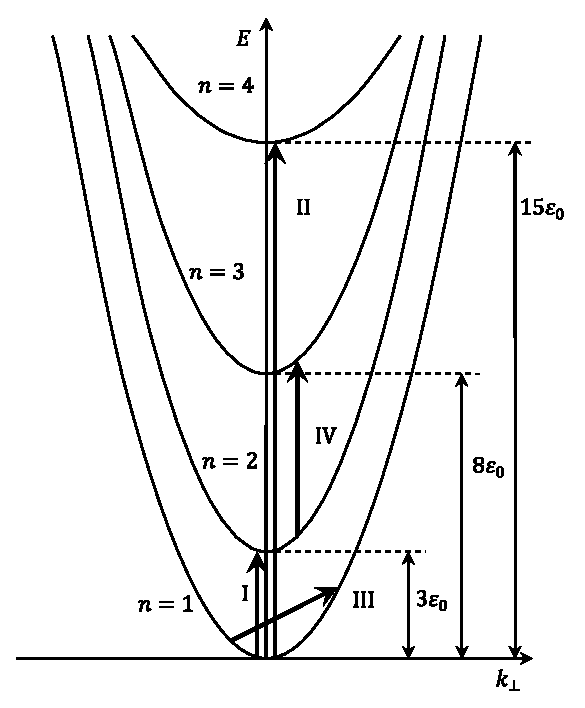
\includegraphics [scale=1] {fig_2_1_1}
	\caption{Энергетическая диаграмма для размерно-квантованной зоны проводимости в размерно-ограниченных системах. Стрелками указаны возможные оптические переходы.} 
	\label{img:fig_2_1_1} 
\end{figure}

В работах \cite{Aleshkin2002,Vorobiev2004} экспериментально, а в \cite{Thammasat1997} теоретически исследовалось межзонное поглощение света в ступенчатых квантовых ямах InGaAs/AlGaAs. При высоких уровнях возбуждения заполняются, как основная подзона, так и возбужденные состояния, что позволило наблюдать поглощение инфракрасного излучения, связанного с переходами электрона между возбужденными состояниями (переход IV на рисунке~\ref{img:fig_2_1_1}). При этом коэффициент поглощения достигает больших значений $(\sim 10^3 \text{ cm}^{-1})$ при высоких температурах $T \simeq 300^{\circ}K$. Влияние поверхности на оптические характеристики в квантовых ямах GaAs/AlGaAs экспериментально исследовалось в \cite{Gurioli1991,Weisbuch1981}. В частности было показано, что учет шероховатой поверхности приводит к уширению спектров фотолюминесценции.

Далее проводится расчет коэффициента поглощения слабой электромагнитной волны $K\left(\Omega \right)$ различной поляризации, как для внутризонных переходов (переход III на рисунке~\ref{img:fig_2_1_1}), так и для межподзонных переходов (переходы I, II) с учетом взаимодействия электронов с шероховатой поверхностью в квантовой яме. При этом коэффициент поглощения электромагнитной волны вычисляется без использования теории возмущений по взаимодействию носителей с шероховатой поверхностью, как это делалось в \cite{Vurgaftman1999}, что позволяет исследовать частотную зависимость $K(\Omega)$ в широкой области частот и сформулировать условия применимости теории возмущений и последовательно описать внутризонное поглощение света и при неслабых взаимодействиях электрона с шероховатой поверхностью.	

Расчет коэффициента поглощения света частоты $\Omega$ и вектора поляризации $\vect{\xi}$ проводится по формуле Кубо \cite{Kubo1957a}, которая в представлении вторичного квантования имеет вид \cite{Sinyavskii2010}:
\begin{multline} \label{eq:21_02}
K(\Omega) = \frac{2 \pi e^2}{V c n_0 \hbar \Omega m_e^2}\left( 1 - e^{-\beta_0 \hbar \Omega} \right) \sum_{\alpha \alpha_1 \beta \beta_1} {\left\langle \alpha \left| (\hat{\vect{P}} \vect{\xi})  \right| \alpha_1 \right\rangle \left\langle \beta \left| (\hat{\vect{P}} \vect{\xi})  \right| \beta_1 \right\rangle} \times\\
\times\int\limits_{-\infty }^{\infty} {dt e^{i\Omega t}\left\langle a_{\alpha }^+ (t) a_{\alpha_1 }(t) a_{\beta }^+ a_{\beta_1 } \right\rangle}  ,
\end{multline} 
${\left| \alpha  \right\rangle} $~---~волновые функции свободного электрона,   $a_{\alpha}^+ (a_{\alpha})$~---~операторы рождения (уничтожения) электрона с эффективной массой $m_e$ в состоянии $\alpha$,  $n_0$~---~показатель преломления, $V$~---~объем основной области квантовой системы,  $\hat{\vect{P}}$~---~оператор импульса, $\beta_0 = 1 / T$,  $T$~---~температура,
\[
a_{\alpha }^+ (t)= \exp\left(\frac{it\hat{H}}{\hbar } \right)a_{\alpha }^+ \exp\left(-\frac{it\hat{H}}{\hbar } \right), \;
\hat{H} = \hat{H}_0 + V, \;
\hat{H}_0 {\left| \alpha  \right\rangle} = E_{\alpha} {\left| \alpha  \right\rangle}.
\]
$V$~---~описывает взаимодействие электрона с шероховатой поверхностью исследуемой наноструктуры шириной $a$ \eqref{eq:1_1}.

Если учесть, что временная зависимость операторов рождения и уничтожения определяется соотношениями \cite{Khamidullin2002}:
\begin{equation} \label{eq:21_04}
a_{\alpha}^+ (t) = \sum_{\gamma}{a_{\gamma}^+ \left\langle \gamma \left| \exp{\left( \frac{it\widetilde{H}}{\hbar}\right) } \right| \alpha \right\rangle},
\end{equation}
\begin{equation} \label{eq:21_06}
a_{\alpha} (t) = \sum_{\gamma}{\left\langle \alpha \left| \exp{\left(- \frac{it\widetilde{H}}{\hbar}\right) } \right| \gamma \right\rangle a_{\gamma}},
\end{equation}  
($\widetilde{H}$~---~гамильтониан рассматриваемой задачи в координатном представлении), то после подстановки \eqref{eq:21_04}, \eqref{eq:21_06} в \eqref{eq:21_02} не трудно получить следующее выражение для коэффициента поглощения слабой электромагнитной волны: 
\begin{multline} \label{eq:21_08}
K(\Omega) = \frac{2 \pi e^2 }{V c n_0 \hbar \Omega m_e^2}\left( 1 - e^{-\beta_0 \hbar \Omega} \right) \int\limits_{-\infty }^{\infty} {dt \sum_{\alpha \alpha_1 \beta \beta_1} {\left\langle \alpha \left| (\hat{\vect{P}} \vect{\xi})  \right| \alpha_1 \right\rangle \left\langle \beta \left| (\hat{\vect{P}} \vect{\xi})  \right| \beta_1 \right\rangle}} \times\\
\times n_{\beta_1} \left(1-n_{\beta} \right)
{\left\lbrace  \left\langle \beta_1 \left| \exp \left(\frac{it\widetilde{H}}{\hbar}\right) \right|\alpha\right\rangle \left\langle \alpha_1 \left| \exp \left(-\frac{it\widetilde{H}}{\hbar}\right) \right|\beta\right\rangle \right\rbrace }_V  .
\end{multline} 
При записи \eqref{eq:21_08} было проведено усреднение по системе свободных электронов; $n_\alpha = \left\{ \exp\left[ \beta \left( \varepsilon _\alpha - \xi \right) \right] + 1 \right\}^{- 1}$~---~равновесная
функция распределения для электронов с энергией $\varepsilon{_\alpha}$, $\xi $~---~химический потенциал.

Не трудно показать, что для прямоугольной квантовой ямы матричные элементы оператора импульса определяются соотношениями $(\alpha (n, \vect{k}{_\bot}), \; \beta (n', \vect{k}'_{\bot}))$:
\begin{equation} \label{eq:21_09_01}
\left\langle \alpha \left| \hat{p}^{(z)} \right| \beta \right\rangle = \frac{2}{a} i\hbar \delta_{k_\bot k'_\bot} \frac{n n_1}{n^2 - n_1^2} \left[(-1)^{n+n_1} -1 \right] , \; n \neq n_1
\end{equation}
\begin{equation} \label{eq:21_09_02}
\left\langle \alpha \left| \hat{p}^{(x)} \right| \beta \right\rangle = \hbar k_x \delta_{\alpha\beta},\;
\left\langle \alpha \left| \hat{p}^{(y)} \right| \beta \right\rangle = \hbar k_y \delta_{\alpha\beta}.
\end{equation} 

Как непосредственно следует из \eqref{eq:21_09_01}, \eqref{eq:21_09_02} поглощение света, связанное с переходами электрона между размерно-квантованными зонами проводимости $n \neq n_1$  (переходы I, II, IV на рисунке~\ref{img:fig_2_1_1}), возможно только в ТМ–поляризации \eqref{eq:21_09_01}. Будем предполагать, что рассеяние электронов на шероховатой поверхности для различных размерно-квантованных зон, между которыми происходит оптический переход, происходит независимо. Усреднение в \eqref{eq:21_08} по реализации случайного процесса проведём с использованием кумулянтного усреднения \cite{Kubo1962}. С точностью до второй кумулянты получаем:
\begin{multline} \label{eq:21_09_04}
I = {\left\lbrace  \left\langle \beta_1 \left| \exp \left(\frac{it\hat{H}}{\hbar}\right) \right|\alpha\right\rangle \left\langle \alpha_1 \left| \exp \left(-\frac{it\hat{H}}{\hbar}\right) \right|\beta\right\rangle \right\rbrace }_V \approx \\
\approx \delta_{\beta_1\alpha} \delta_{\alpha_1\beta} \exp{\left[\frac{it}{\hbar} \left(E_{\alpha} - E_{\alpha_1} \right)  \right] } \exp{\left[- g_{\alpha\alpha_1}(t) \right]}
\end{multline} 
\begin{multline} \label{21_09_06}
g_{\alpha\alpha_1 }(t)=\frac{1}{{\hbar }^2}\int\limits_0^t d \tau \int\limits_0^{\tau }d \tau_1 \sum_{\gamma} \left\{ W_{\alpha\gamma }\exp \left[\frac{i}{\hbar }\left(\tau_1-\tau \right) \left(E_{\alpha}-E_{\gamma }\right)\right] + \right.\\
\left. + W_{\alpha_1\gamma} \exp \left[\frac{i}{\hbar }\left(\tau_1-\tau \right)\left(E_{\alpha_1}-E_{\gamma }\right)\right] \right\}
\end{multline} 

В результате, если использовать приближение времени релаксации \eqref{eq:31_130}, и пренебречь поправками к энергии свободных электронов, связанными с рассеяниями носителей на шероховатой поверхности, не трудно получить:
\begin{equation} \label{eq:21_09_08}
I = \delta_{\beta_1\alpha} \delta_{\alpha_1\beta} \exp{\left[\frac{it}{\hbar} \left(\widetilde{E}_{\alpha} - \widetilde{E}_{\alpha_1} \right)  \right] } \exp{\left(- \frac{|t|}{\tau_{\alpha\alpha_1}} \right)}.
\end{equation}
Здесь введены следующие обозначения:
\[
\widetilde{E}_{\alpha} = E_{\alpha} - \frac{W_{\alpha \gamma}}{E_{\alpha} - E_{\gamma}}
\]
\[
W_{\alpha\beta}=\int{d\vect{r} d\vect{r_1} \Psi^*_\alpha(\vect{r}) \Psi^*_\beta(\vect{r_1}) V_\alpha V_\beta F \Psi_\alpha(\vect{r_1}) \Psi_\beta(\vect{r})}
\]
\[
\frac{1}{\tau_{\alpha\alpha_1}} = \frac{\pi}{\hbar} \sum_{\gamma } { \left[W_{\alpha \gamma }\delta \left(E_{\alpha} - E_{\gamma}\right) + W_{\alpha_1 \gamma }\delta \left(E_{\alpha_1} - E_{\gamma}\right) \right] }
\]
Для случая $\delta$-коррелированной флуктуации поверхности
\begin{equation} \label{eq:21_09_10}
\frac{1}{\tau_{\alpha\alpha_1}} = \frac{1}{\tau_0} \left(n^4 + n_1^4 \right) ,
\end{equation}
\[
\frac{1}{\tau_0}  = \frac{m_e}{2\hbar^3} \left(\frac{2\varepsilon_0}{a} \right)^2 \gamma_0. 
\]
Из \eqref{eq:21_09_10} следует, что время релаксации при рассеянии носителей на шероховатой поверхности не зависит от волнового вектора электрона и заметным образом уменьшается с ростом $n$ и $n_1$. Для невырожденного электронного газа, если использовать соотношения \eqref{eq:21_08} и \eqref{eq:21_09_10}, то коэффициент поглощения света, связанный с переходом электрона из нижайшей зоны проводимости $(n=1)$ в ближайшую размерно-квантованную зону проводимости $(n_1=2)$ (переход I на рисунке~\ref{img:fig_2_1_1}), записывается следующим образом $(\beta _0\hbar \Omega \gg 1)$:
\begin{equation} \label{eq:21_10}
K(\Omega) = K_M \frac{1}{1+\left(\dfrac{\tau_0 }{17 \hbar} \Delta_0 \right)^2 } ;
\end{equation} 
\[
K_M =\frac{2^{12} e^2 a^5 n_e }{\hbar cn_0 \pi^5 \gamma_0 3^3 \cdot 17}, \;
\Delta_0 =\hbar \Omega -3\varepsilon_0.
\]
$n_e =N/L_x L_y $~---~поверхностная плотность электронов. При записи (\ref{eq:21_10}) учитывалось, что в размерно-квантованной зоне, на которую происходит оптический переход носителя, электронов нет, поэтому $n_{\beta } \ll 1$. Последнее приближение вполне справедливо, если  $3\varepsilon_0 \gg kT$, т.е. почти все электроны находятся на нижайшей размерно-квантованной зоне проводимости $(n=1)$, и, следовательно, $\sum n_{k_{\bot } } \cong N$ ($N$~---~число электронов в исследуемой квантовой системе). Из \eqref{eq:21_10} следует, что частотная зависимость коэффициента поглощения света описывается лоренцовой кривой с полушириной  $\delta =17\cdot 2\hbar /\tau_0 $. Величина коэффициента поглощения электромагнитной волны при рассматриваемом механизме рассеяния существенным образом определяется толщиной квантовой ямы $\left(K_M \sim a^5 \right)$ и не зависит от температуры. $K\left(\Omega \right)$  в максимуме при $n_e =4\cdot 10^{11} \text{cm}^{-2} $, $n_0 = 3.2$,   принимает значение   $K_M^{\left(\delta \right)} =0.25\cdot a_0^5 /\gamma_0 $ ($a_0 $, $\sqrt[4]{\gamma_0}$~--–~измеряются в ангстремах), т.е. при  $a_0 = 80 \AA$,  $\sqrt[4]{\gamma_0} = 10 \AA$ (именно такие значения   хорошо описывают значения подвижности   экспериментально наблюдаемые в КЯ GaAs/AlGaAs \cite{West1985}), $K_M =2\cdot 10^4 \text{cm}^{-1} $. Большие значения коэффициента поглощения света позволяют надеяться на практическое использование таких размерно-квантованных систем в качестве детекторов ИК-излучения в области низких температур. Полуширина линии поглощения для рассматриваемого прямого оптического перехода при рассматриваемых выше параметрах $\delta =6.5\cdot 10^6 \left(\gamma_0 /a_0^6 \right)\text{meV}$. Следовательно, при  $a_0 = 60 \AA$,  $\sqrt[4]{\gamma_0} = 15 \AA$,  $\delta = 7 \text{ meV}$, что безусловно, находится в области экспериментального измерения.

Для ТЕ-поляризованного излучения, из \eqref{eq:21_09_02} следует, что  возможно поглощение света только в одной размерно-квантованной зоне проводимости (переход III на рисунке~\ref{img:fig_2_1_1}). В этом случае функция \eqref{21_09_06} после интегрирования по $\tau$ и $\tau_1$ может быть записана следующим образом:
\begin{equation} \label{eq:21_09_12}
g_{\alpha\alpha_1 }(t) =2 \sum_{\gamma}  \frac{ W_{\alpha\gamma }}{\left(E_{\alpha} - E_{\gamma} \right)^2 } \left[1 - \cos{\frac{t}{\hbar} \left( E_{\alpha} - E_{\gamma} \right) } \right] .
\end{equation}

Рассмотрим поглощение слабой электромагнитной волны в нижайшей $(n=1)$ размерно-квантованной зоне. Если провести суммирование в \eqref{eq:21_09_12} по $\gamma$ $\left( E_{\gamma} = \varepsilon_0 + \hbar^2 {k'}_{\bot}^2 / {2m_e} \right) $ и подставить $g_{\alpha\alpha_1 }(t)$ в \eqref{eq:21_08}, то выражение для коэффициента поглощения света в случае невырожденного электронного газа принимает вид:
\begin{multline} \label{21_09_14}
K(\Omega) = \frac{2 \pi e^2 n_e }{m_e c n_0 a \hbar \beta_0 \Omega^2} \int\limits_0^{\infty}x dx \int\limits_{-\infty}^{\infty}y dy \times \\
\times \exp{\left\lbrace  - 2\Gamma_0 |y| \left[ 1 - \frac{\delta_0}{\pi x |y|}\sin^2{\left( \frac{x|y|}{\delta_0}\right) } + \frac{1}{\pi} \mathrm{Si}{\left( \frac{2x|y|}{\delta_0}\right) } \right]  \right\rbrace   }.
\end{multline} 
Здесь введены следующие обозначения:
\[
\delta_0 = 2\hbar \Omega \beta_0,
\]
\[
\Gamma_0 = \pi^2 \left(\frac{\varepsilon_0}{\hbar \Omega} \right) \left( \frac{\gamma_0}{a^4} \right),
\]
\[
\mathrm{Si}(z) = -\frac{\pi}{2} + \int\limits_0^z{d\tau\frac{\sin{t}}{\tau}}.
\]

В случае низких температур выражение для поглощения света \eqref{21_09_14} можно записать:
\begin{equation} \label{eq:21_20}
K(\Omega )=\frac{4\pi e^{2} n_{e} }{m_e c n_0 a \hbar\beta \Omega^2 } \frac{\Gamma_0 }{1+\Gamma_0^2 }
\end{equation} 

Как показывают численные расчеты, соотношение \ref{eq:21_20} при больших $\delta_0$ мало отличается от точного \ref{eq:21_20}. Например, при $\delta_0 > 5$ отличие менее 10\% в широком интервале изменения $\Gamma_0$. Заметим, что в нижайшем приближении по взаимодействию электрона с шероховатой поверхностью $\Gamma_0 \ll 1$, что соответствует обычной теории возмущений, тогда из (\ref{eq:21_20}) нетрудно получить:
\begin{equation} \label{eq:21_30}
K(\Omega )=\frac{2^4 e^2 n_e \gamma_0 m}{\pi c n_0 a\hbar^3 \beta_0 } \left(\frac{\varepsilon_0 }{\hbar\Omega } \right)^3
\end{equation} 

В рассматриваемом случае $K(\Omega )\sim \Omega^{-3} $ и при низких температурах ($T=50 K$) для $\gamma_0^{1/4} =15 \AA$, $n_e = 2\cdot 10^{12} \text{cm}^{-2} $, $a=50 \AA$, $K_0 (\Omega )\cong 10\left(\varepsilon_0 / \hbar\Omega \right)^3 \text{cm}^{-1} $.

При $\Gamma_0 \gg 1$, что соответствует сильному взаимодействию электрона с шероховатой поверхностью, коэффициент внутризонного поглощения электромагнитной волны определяется соотношением:
\begin{equation} \label{eq:21_40}
K(\Omega )=\frac{2^4 e^2 n_e a}{\pi^3 cn_0 \hbar } \frac{1}{\delta_0 } \left(\frac{a^4 }{\gamma_0 } \right)
\end{equation} 

В рассматриваемом приближении сильной связи $a^4 /\gamma_0 =1$, $K(\Omega )\sim \Omega ^{-1} $ и для $\delta_0 =10$, $a=50 \AA$, $K(\Omega )\cong 120 \text{ cm}^{-1} $. Следовательно, в области низких частот для узких квантовых ям с большой флуктуацией поверхности теория возмущений при исследовании внутризонного поглощения света может оказаться несправедливой.
	

\section{Влияние лазерного излучения на оптические свойства квантовых пленок} \label{sect2_2}

Исследования резонансных явлений в физике твердого тела являются довольно привлекательными, так как в этом случае лазерное излучение приводит к заметному влиянию на кинетические явления даже при небольших интенсивностях электромагнитной волны. Примером может служить влияние инфракрасного (ИК) лазерного излучения частоты $\omega $ на коэффициент межзонного магнетопоглощения слабого света, когда $\omega $ равна циклотронной частоте $\omega_c $ (магнитоинфракрасный резонанс -- МИКР). В этом случае резонансное ИК-излучение оказывается причиной нестационарности электронных состояний и может полностью определять форму пиков магнетопоглощения слабой электромагнитной волны при небольших интенсивностях лазерного излучения. Наиболее ярко резонансные эффекты в кинетических коэффициентах могут проявляться в размерно-квантованных системах (параболические квантовые ямы), когда частота ИК лазерного излучения равна частоте размерного квантования (размерно-инфракрасный резонанс -- РИР). В частности, экспериментальное обнаружение влияния РИР на межзонное поглощение слабого света позволит не только обосновать используемые модели, но и говорить о совершенстве этих размерно-квантованных систем. В этом параграфе исследуется влияние постоянного электрического поля на межзонное поглощение слабой электромагнитной волны в режиме МИКР и РИР. Именно в постоянном электрическом поле, во-первых, наиболее отчетливо проявляются эффекты влияния на коэффициент поглощения света резонансного лазерного излучения и, во-вторых, возникают дополнительные особенности в высокочастотной области спектра поглощаемой электромагнитной волны.

Если магнитное поле $\vect{H}||OZ$, электрическое поле направлено вдоль $\vect{H}$, то гамильтониан для электрона в калибровке Ландау $A(-Hy,0,0)$ в поле лазерного излучения примет вид:

\begin{multline} \label{eq:22_10} 
\hat{H}_c =\frac{1}{2m_c } \hat{P}^2 +\frac{e}{m_e c} (\hat{P}\xi )\sqrt{\frac{4\pi c^2 }{V} } (\hat{b}+\hat{b}^+ ) + \\ 
+\frac{e^{2} }{2m_e c^2 } \left(\frac{4\pi c^{2} }{V} \right)(\hat{b}+\hat{b}^+ )^2 +\hbar \omega \hat{b}^+ \hat{b}+eEz\equiv \hat{H}_c^0 +eEz,
\end{multline}
где $\hat{P}=\hat{p}+\frac{e}{c} \hat{A}$; $\hat{b}^+ (\hat{b})$~---~операторы рождения (уничтожения) для интенсивного лазерного излучения частоты $\omega $, поляризации $\xi $; $V$~---~объем основной области кристалла; $m_e $~---~эффективная масса электрона.

Коэффициент межзонного поглощения слабой электромагнитной волны частоты $\Omega $ и поляризации $\xi _{0} $ согласно формуле Кубо \cite{Kubo1957a} можно привести к виду \cite{Sokovnich2004}:
\begin{multline} \label{eq:22_20} 
K(\Omega )=\frac{4\pi e^2 }{V n_0 c\hbar \Omega } \left|\frac{p_{cv} \xi_0 }{m_0 } \right|^2 \times  \\
\times \sum _{\beta } \int\limits_{-\infty }^{\infty} dt \exp \left(i\Omega t-\frac{i e^2 E^2 t^3 }{6\hbar \mu } +\frac{ieEk_z t^2}{2\mu } \right)\times  \\ 
\times \left\{<\beta^c |\exp \left(\frac{it}{\hbar } \hat{H}_v^0 \right)\exp \left(-\frac{it}{\hbar } \hat{H}_c^0 \right)|\beta^c >\right\}_f  
\end{multline} 
где $|\beta^c >$~---~волновые функции для электронов в зоне проводимости в отсутствии электрического поля; $\beta $~---~набор квантовых чисел, описывающих состояние заряженной частицы; $p_{cv} $~---~матричный элемент оператора импульса на блоховских функциях, $\mathop{\hat{H}}\nolimits_i^0 $~---~гамильтониан для электронов в магнитном поле в $i$-ой зоне ($i=c,v$); $\{ \}_f$~---~описывает усреднение по системе свободного фотонного поля \cite{Glauber1963,Klauder1968}. 

Далее исследуем случай, когда электрическое поле $\vect{E_0} $ линейно-поляризованного лазерного излучения перпендикулярно $\vect{H}$, т.е. лазерное излучение распространяется вдоль $\vect{H}$. Именно в такой поляризации интенсивная электромагнитная волна смешивает ближайшие уровни Ландау. Дальнейшие расчеты, для простоты, проводятся в резонансном приближении $\omega_c =eH/(m_c c)=\omega $ (магнитоинфрокрасный резонанс МИКР), и поэтому не учитывается взаимодействие дырок с лазерным излучением ($\omega_v =eH/(m_v c)\ne \omega $, $m_v \gg m_c $). В рассматриваемом приближении третьим слагаемым в \eqref{eq:22_10}, описывающим двухфотонные процессы, пренебрегаем. В результате, проводя расчет методом, использованным в \cite{Sinyavskii1974,Sinyavskii2002}, нетрудно получить: 
\begin{multline} \label{eq:22_30} 
K(\Omega )=\frac{2e^2 }{n_0 c\hbar R^2 } \left|\frac{p_{cv} \xi_0 }{m_0 } \right|^2 \sqrt{\frac{2\mu }{\pi \hbar \omega } } \frac{1}{\gamma^{\tfrac{1}{4}}} \times \\
\times \sum_n \int\limits_0^{\infty } \frac{d\tau }{\sqrt{\tau } } \cos \left(a\tau ^3 -\Delta_n \tau +\frac{\pi }{4} \right)\exp \left(-\frac{\tau^2 }{2} \right)L_n (\tau^2 )
\end{multline} 
где 
\[
\Delta_n =\frac{\hbar \Omega -E_g -\hbar \omega^* \left(n+\tfrac{1}{2} \right)}{\hbar \omega \sqrt{\gamma } } ; \; a=\frac{e^2 E^2 }{2 4\mu \omega^3 \hbar \gamma^{\tfrac{3}{2}}} ; \; \gamma =\frac{e^2 E_0^2 }{8 \mu \hbar \omega^3 } ;
\] 
$\mu^{-1} =m_c^{-1} +m_v^{-1} ;$~~$\omega^* =\omega_c +\omega_v ;$~~$L_n(z)$~---~полиномы Лагерра; $E_g $~---~ширина запрещенной зоны; $n$~---~номер уровня Ландау. 
Как следует из \eqref{eq:22_30}, в поле резонансного ИК лазерного излучения $(\omega_c =\omega )$ возникает затухание гауссовского типа $\exp \left(-\tau^2 /2\right)$, т.е. лазерное излучение приводит к нестационарности электронных состояний. При записи \eqref{eq:22_30} пренебрегалось влиянием электрон--фононного взаимодействия на форму линии магнетопоглощения. Как показали детальные исследования в работе \cite{Sinyavskii1976} это вполне оправдано для реальных полупроводниковых материалов даже при небольших интенсивностях резонансного ИК лазерного излучения. 

\begin{figure}[!h] 
	\center
	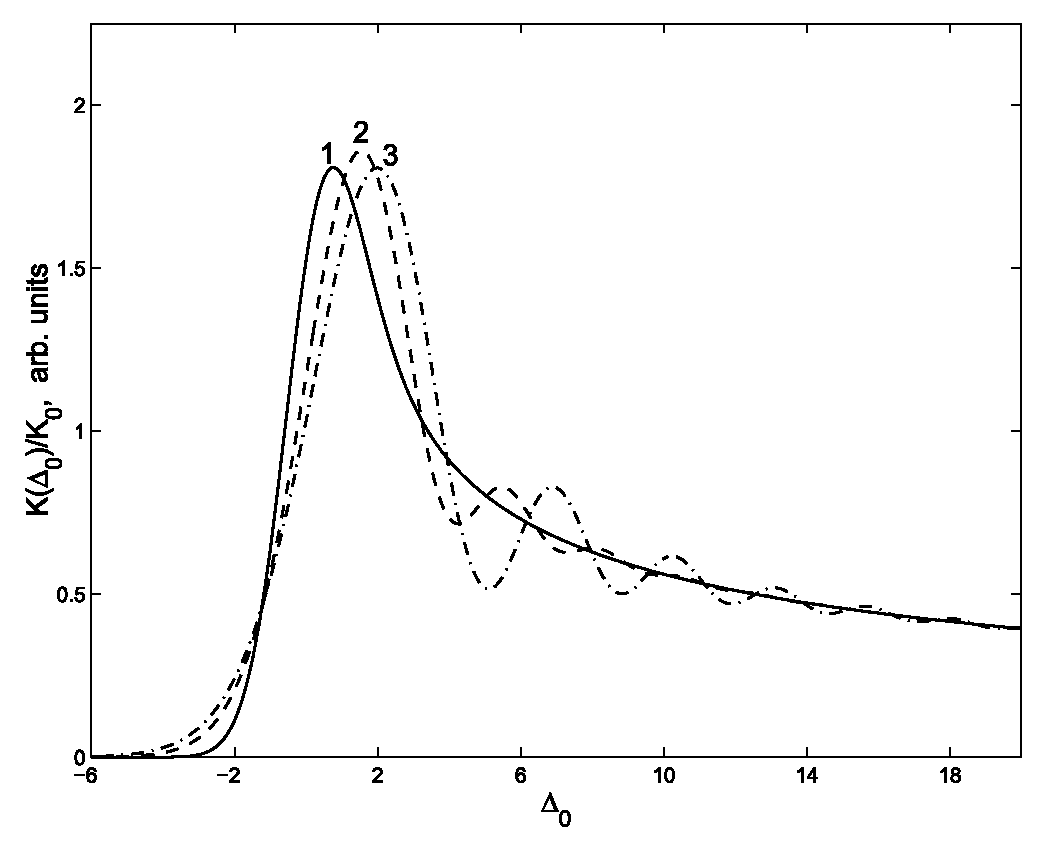
\includegraphics [scale=0.8] {fig_2_2_1}
	\caption{Частотная зависимость первого пика магнетопоглощения в режиме магнитоинфракрасного резонанса. Кривые 1, 2, 3 получены соответственно для $a=0$; $a=0.4$; $a=0.8$.} 
	\label{img:fig_2_2_1} 
\end{figure}

\begin{figure}[!h] 
	\center
	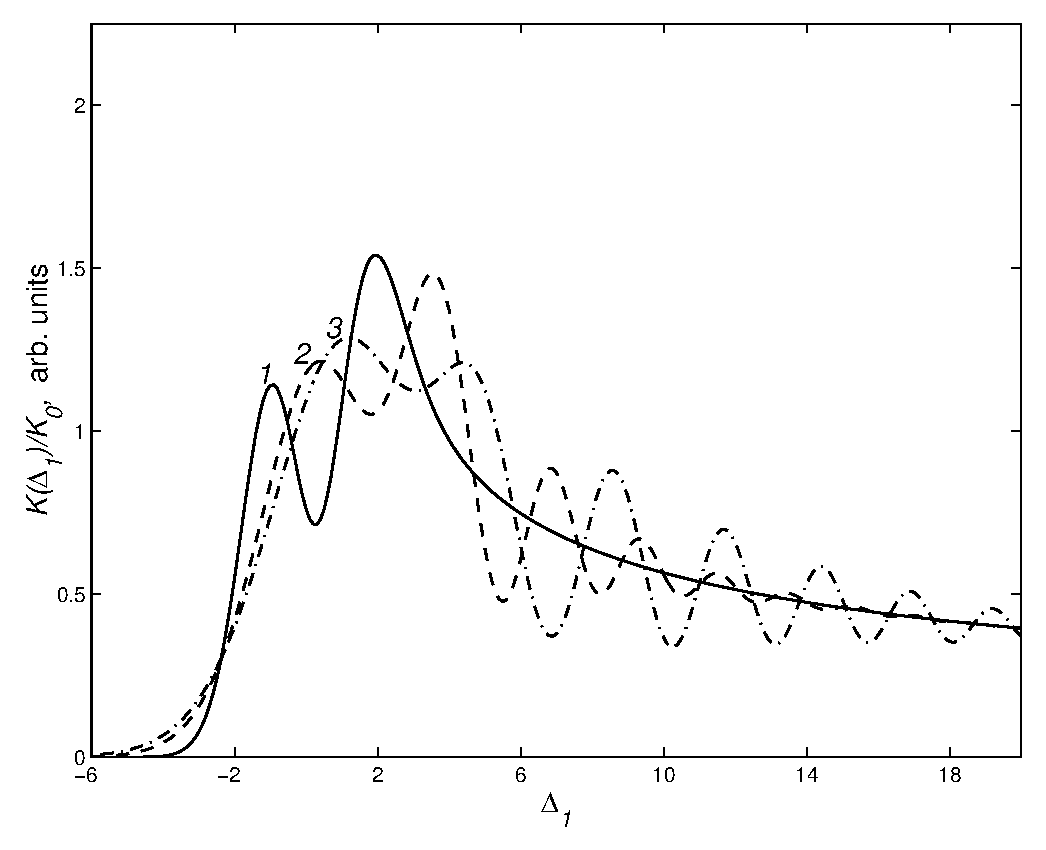
\includegraphics [scale=0.8] {fig_2_2_2}
	\caption{Частотная зависимость второго пика магнето-поглощения в режиме магнитоинфракрасного резонанса. Кривые 1, 2, 3 получены соответственно для $a=0$; $a=0.4$; $a=0.8$.} 
	\label{img:fig_2_2_2} 
\end{figure}

На рисунке~\ref{img:fig_2_2_1} представлены частотные зависимости линии магнетопоглощения в относительных единицах для $n=0$, т.е. для оптических переходов между нижайшими уровнями Ландау валентной зоны и зоны проводимости при различных значениях постоянного электрического поля. Кривые 1, 2, 3 получены соответственно для $a=0$, $a=0.4$, $a=0.8$.

Из представленных результатов видно, что с ростом напряженности электрического поля величина первого пика магнетопоглощения уменьшается, полуширина увеличивается, и в высокочастотной области возникают осцилляции коэффициента поглощения света. При переходе электрона на первый уровень Ландау (в формуле \eqref{eq:22_30} $n=1$) частотная зависимость второго пика магнетопоглощения описывается двумя пиками, причем величина длинноволнового пика меньше величины пика в высокочастотной области спектра (рисунок~\ref{img:fig_2_2_2}, кривая 1 получена при $a=0$). С ростом напряженности однородного электрического поля величина коротковолнового пика уменьшается, и в высокочастотной области возникают характерные осцилляции коэффициента поглощения света (кривые 2, 3 на рисунке~\ref{img:fig_2_2_2} получены при $a=0.4$, $a=0.8$ соответственно). 

Теперь рассмотрим межзонное поглощение слабой электромагнитной волны в параболических квантовых ямах, в которых благодаря размерному квантованию возникают эквидистантные зоны проводимости и валентные зоны. Если электрическое поле линейно-поляризованного излучения направлено вдоль оси пространственного квантования, то инфракрасное лазерное излучение смешивает ближайшие эквидистантные зоны.

Вычислим коэффициент межзонного поглощения слабого света, когда частота лазерного излучения $\omega $ равна частоте размерного квантования $\omega_c $ в зоне проводимости (размерно-инфракрасный резонанс -- РИР), а напряженность $E$ постоянного электрического поля направлена параллельно поверхности параболической квантовой ямы (ПКЯ). Коэффициент поглощения света $K(\Omega )$ вычисляется так же, как это было сделано выше и с учетом тех же приближений принимает следующий вид: 
\begin{multline} \label{eq:22_40} 
K(\Omega )=K_0 \sum _{n} \, V_n^2 \times  \\
\times \left\{\frac{\pi }{2} +\int_0^{\infty } dt \exp \left(-\frac{x^2 }{2} \right)L_n \left(x^2 \right)\frac{\sin \left[x\left(\Delta_n -\delta x^2 \right)\right]}{x} \right\}
\end{multline} 
где 
\[\Delta_n =\frac{\hbar \Omega -E_g -\hbar \omega^* \left(n+{\tfrac{1}{2}} \right)}{\hbar \sqrt{\gamma } } ; \; \omega^* =\omega_c +\omega_v ;\] 
$\hbar \omega_v $~---~энергия размерного квантования в валентной зоне, $V_n $~---~матричный элемент волновых функций электрона в зоне проводимости и в валентной зоне для ПКЯ \cite{Sinyavskii2002}. В отсутствии постоянного электрического поля $(E=0)$ \eqref{eq:22_40} переходит в выражение для межзонного поглощения света в режиме РИР, полученного в \cite{Sinyavskii2002}. В частном случае 
\[V_0 =\mathop{\left(\lambda_c \lambda_v \right)}\nolimits^{{\tfrac{1}{4}} } \sqrt{\frac{2}{\lambda_c +\lambda_v } } ;\; \; V_1 =2\sqrt{2} \frac{\mathop{\left(\lambda_c \lambda_v \right)}\nolimits^{{\tfrac{3}{4}} } }{\mathop{\left(\lambda_c +\lambda_v \right)}\nolimits^{{\tfrac{3}{2}} } } ;\; \; \lambda_i =\frac{m_i \omega^i }{\hbar } (i=c,v).\] 
Для типичных параметров ПКЯ GaAs-AlGaAS $\lambda_c /\lambda_v =0.47$ ($m_c =0.06m_0 ,$ $m_v =0.4m_0 $). На рисунке~\ref{img:fig_2_2_3} приведена частотная зависимость коэффициента межзонного поглощения света (в относительных единицах) при переходе электрона из нулевого (первого $n=1$) размерно-квантованного состояния валентной зоны на нулевое $n=0$ (первое $n=1$) размерно-квантованное состояние зоны проводимости. Кривая 1 описывает частотную зависимость коэффициента поглощения в отсутствии постоянного электрического поля \cite{Sinyavskii2002}. Кривая 2 получена при $a=0.4$, кривая 3 при $a=0.8$. Из рисунка~\ref{img:fig_2_2_3} видно, что постоянное продольное электрическое поле существенным образом влияет на межзонный коэффициент поглощения света. При этом в электрическом поле возможно заметное поглощение в длинноволновой области спектра, а в высокочастотной области поглощение света определяется характерной осцилляционной зависимостью от частоты. С ростом напряженности постоянного электрического поля осцилляции становятся наиболее отчетливыми. 
\begin{figure}[!h] 
	\center
	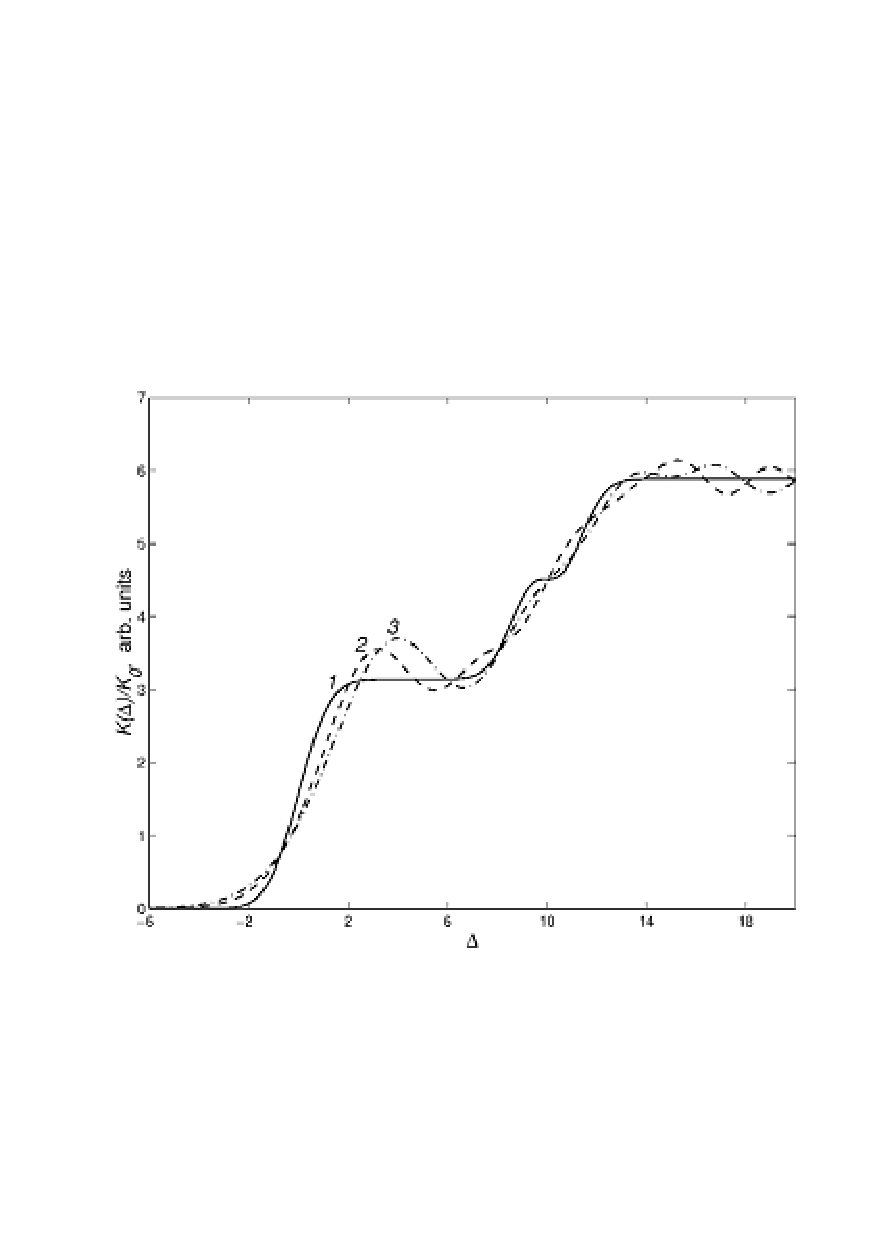
\includegraphics [scale=0.8] {fig_2_2_3}
	\caption{Частотная зависимость межзонного поглощения света в режиме размерно-инфракрасного резонанса. Кривые 1, 2, 3 получены соответственно для $a=0$; $a=0.4$; $a=0.8$.} 
	\label{img:fig_2_2_3} 
\end{figure}


\section{Оптические свойства квантовых проволок в присутствии резонансного лазерного излучения} \label{sect2_3}

Теперь исследуем явления, связанные с МИКР и размерно-инфракрасным резонансом (РИР) в квантовой проволоке в однородном магнитом поле $\vect{B}$ $(\vect{B} \parallel OZ)$, направленном перпендикулярно оси исследуемой наноструктуры с учетом взаимодействия носителей с шероховатой поверхностью. Такие одномерные структуры интересны тем, что имеют особенности в плотности энергетических состояний на дне размерно-квантованных зон, приводящие к особенностям оптических свойств. Энергетический спектр электрона в параболической нанопроволоке известен \cite{Hashimzade2005}:
\[
E_{\alpha }=\frac{\hbar^2 k^2_x}{2m^*_e}+\hbar \Omega_e\left(n+\frac{1}{2}\right)+\hbar {\omega }_e\left(m+\frac{1}{2}\right)
\] 
\[
m^*_e=m_e{\left(\frac{\Omega_e}{\omega_e}\right)}^2,\;
\Omega_e={\left[{\omega }^2_e+{\omega_c}^2\right]}^{1/2},\;
\omega_c=\frac{eB}{m_ec\ }
\] 
$\hbar\omega_e$~--~энергия размерного квантования электрона массы $m_e$ в зоне проводимости, $\omega_c$~--~циклотронная частота. Аналогично можно записать энергию для электрона в валентной зоне.

\begin{figure}[!h] 
	\center
	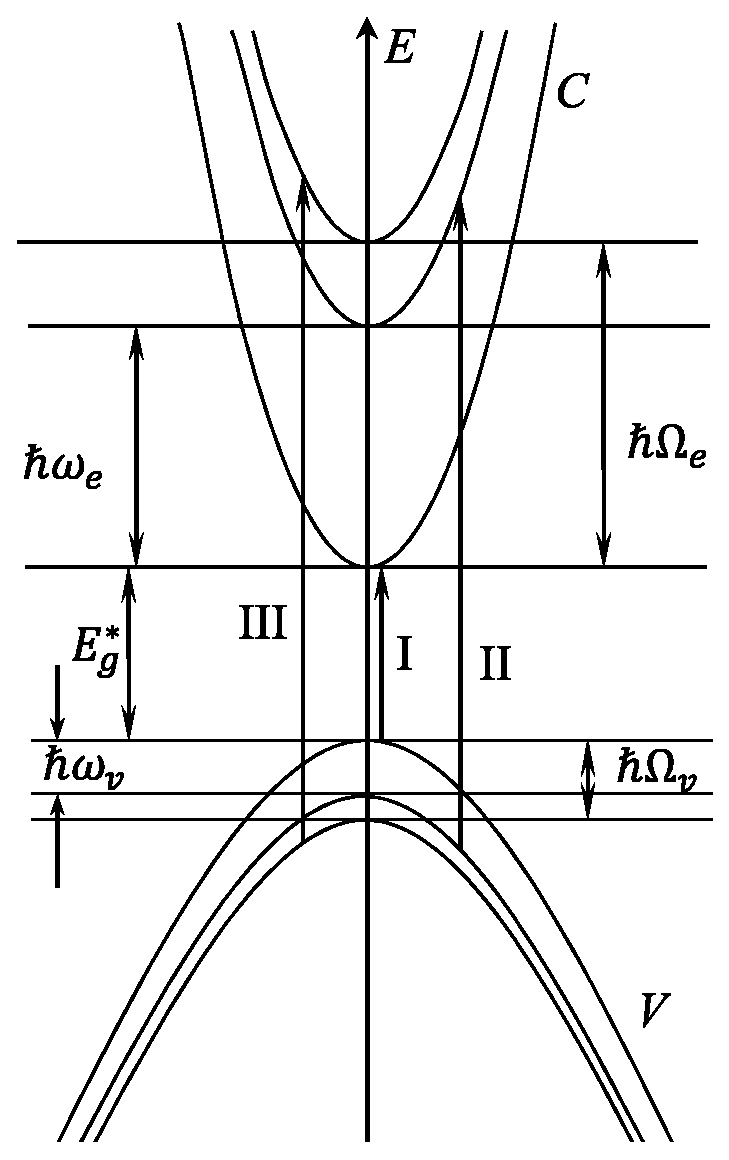
\includegraphics [scale=0.6] {fig_2_3_1}
	\caption{Схема энергетических зон полупроводниковой квантовой проволоки в поперечном магнитном поле и оптические переходы.} 
	\label{img:fig_2_3_1} 
\end{figure}

Будем исследовать оптические свойства полупроводниковых квантовых проволок (КП), схема энергетических зон которых изображена на рисунке~\ref{img:fig_2_3_1} $E^*_g$~---~ширина запрещенной зоны КП в магнитном поле, $\omega_v, \Omega_v$~---~соответственно частота размерного квантования и гибридная частота носителей в валентной зоне.

Вычислять коэффициент межзонного поглощения слабой электромагнитной волны в поле лазерного излучения, будем в случае, когда его частота $\omega_L$ равна $\omega_e$ частоте размерного квантования (РИР) или $\Omega_e$ (магнитно-инфракрасный резонанс). Так как для типичных полупроводниковых наноструктур эффективная масса электронов в зоне проводимости значительно меньше массы дырок ($m_e\ll m_v$), то взаимодействием интенсивного ИК излучения с электронами в валентной зоне в дальнейшем пренебрегаем ($\omega_e\gg \omega_v\ $).

Гамильтониан в представлении вторичного квантования для электронов в зоне проводимости в состоянии $\alpha $ в поле одномодового лазерного излучения поляризацией $\vect{\xi}$ записывается в следующем виде:
\begin{equation} \label{eq:23_10} 
\hat{H}=\sum_{\alpha } {\varepsilon_{\alpha } a^+_{\alpha } a_{\alpha }} + \hbar \omega_L b^+ b + {\left[\frac{2\pi \hbar e^2} {V \omega_L} \right]}^{\frac{1}{2}} {\sum_{\alpha \alpha_1}{\left|\frac{\vect{P}_{\alpha \alpha_1} \vect{\xi}}{m_e}\right|}}^2 a^+_{\alpha } a_{\alpha_1} (b^+ + b).
\end{equation}
Здесь $a^+_{\alpha }\ (a_{\alpha })$, $b^+ (b)$ -- операторы рождения (уничтожения) электронов в состоянии $\alpha $ и фотонов.

Расчет матричных элементов оператора импульса $\vect{P}_{\alpha\alpha_1}$ на волновых функциях параболической квантовой проволоки в продольном магнитном поле \cite{Hashimzade2005} не представляет труда. В результате:
\begin{equation} \label{eq:23_20}
\begin{aligned}
&{\left| P^X_{\alpha \beta }\right|}^2=\frac{\delta^2}{\sqrt{\left(1+\delta^2\right)} }{\left|P^Y_{\alpha \beta }\right|}^2, \;
\delta =\frac{\omega_c}{\omega_e},\\
&\left| P^Y_{\alpha \beta }\right|^2=
\frac{m_e \sqrt{\left({1+\delta }^2\right)} \hbar\omega_e}{2} \left[  n \delta_{n,n_1+1} + (n+1) \delta_{n,n_1-1} \right]\delta_{k_x,k_x'}\delta_{m,m_1} , \\
&{\left| P^Z_{\alpha \beta }\right|}^2=\frac{m_e \hbar\omega_e}{2} \left[ m \delta_{m,m_1+1} + (m+1){\delta }_{m,m_1-1} \right]  \delta_{k_x,k_x'} \delta_{n,n_1}.
\end{aligned}
\end{equation}

Из выражения \eqref{eq:23_20} следует, что линейно X-поляризованная волна лазерного излучения (электромагнитная волна распространяется перпендикулярно оси нанопроволоки) в отсутствии магнитного поля $(\delta =0)$ не взаимодействует с зонными носителями. Согласно \eqref{eq:23_20} линейно Y-поляризованная волна (лазерное излучение распространяется вдоль оси квантовой проволоки) смешивает гибридные состояния $\left( \hbar\omega_L = \hbar\Omega_e \right) $, а Z-поляризованная волна (напряженность электрического поля лазерного излучения $\vect{E}\bot \vect{B}$) смешивает только размерно-квантованные состояния $ \left( \hbar\omega_L = \hbar\omega_e \right) $.

Расчет коэффициента межзонного поглощения слабой электромагнитной волны частоты $\Omega$ в поле резонансного лазерного излучения для квантовых проволок производился с использованием формулы Кубо \cite{Kubo1957a} и методики, развитой в \cite{Sinyavskii1974}. В результате при $\omega_L = \Omega_e$ (резонансный случай) для стабильно генерирующего ИК лазерного излучения Y-поляризации получаем:
\begin{multline} \label{eq:23_30}
K\left(\Omega\right)=K_0{\sum_{nm}{\left|\left\langle \alpha_c | \alpha_v \right\rangle \right|}}^2 
\int\limits_{-\infty }^{\infty }dk_x \int\limits_{-\infty }^{\infty }{dt \exp{\left( -a t^2 -\frac{\Gamma_0 }{\left|k_x\right|}|t| \right) }} L_n\left(2at^2 \right)\times\\
\times {\exp \left\{\frac{it}{\hbar }\left[\hbar \Omega-E^*_g-\frac{\hbar^2 k^2_x}{2\mu^*}-m\left(\hbar\omega_e+\hbar\omega_v\right)-n\left(\hbar\Omega_e + \hbar\Omega_v \right)\right]\right\}\ }
\end{multline}
\[
K_0=\frac{\hbar \Omega e^2}{4\mu^* E_g^* n_0 c s}, \;
a=\frac{e^2 E^2}{8 m_e \hbar\Omega_e},
\]
\[
\frac{1}{\mu^*}=\frac{1}{m^*_e}+\frac{1}{m^*_v},\;
m^*_v=m_v {\left(\frac{\Omega_v}{\omega_v}\right)}^2
\] 
$\left\langle \alpha_c | \alpha_v \right\rangle $~---~матричный элемент сглаженных волновых функций электрона в зоне проводимости и в валентной зоне, $L_n\left(z\right)$~---~полиномы Лаггера, $E$~---~напряженность электрического поля лазерного излучения, $s$~---~сечение квантовой проволоки. 

При записи \eqref{eq:23_30} учитывалось взаимодействие носителей с шероховатой поверхностью или с длинноволновыми акустическими фононами в приближении времени релаксации \cite{Khamidullin2002}. ${\Gamma_0}/{\left|k_x\right|}$~--~описывает вероятность рассеяния электронов в единицу времени или на шероховатой поверхности \eqref{eq:1_19}, \eqref{eq:1_20}  или упругое рассеяние на акустических фононах \cite{Khamidullin2006}.

Запишем коэффициент поглощения света, связанный с переходом электрона из нижайшей валентной зоны $(m=n=0)$ в нижайшую размерно-квантованную зону проводимости $(n=m=0)$. (Оптический переход I на рисунке~\ref{img:fig_2_3_1}) Интегрирование по $t$ в  \eqref{eq:23_30} проводится точно, в результате, после замены
\[
\frac{{\hbar }^2 k^2_x}{2\mu^*}=\hbar {\omega }_fx^2, \left({\omega }^3_f = \frac{\hbar {\gamma }^2_0}{2\mu^*}\right)
\] 
соотношение  \eqref{eq:23_30} записывается в виде $\left(L_0\left(z\right)=1\right)$:
\begin{equation} \label{eq:23_40}
K\left(\Omega\right)=K_0\sum_{nm}{ {\lvert\langle \alpha_c | \alpha_v \rangle\rvert}^2 {\left[\frac{8\pi \mu^*\omega_f}{\hbar a}\right]}^{\frac{1}{2}} \mathrm{Re} \int\limits_0^\infty {dx e^{f^2\left(x\right)}\left[1-\Phi \left(f\left(x\right)\right)\right]}}
\end{equation}
\[
\Phi \left(z\right)=\frac{2}{\sqrt{\pi}}\int\limits_0^z {e^{-\tau^2}}d\tau ,
\] 
\[
f\left(x\right)={\left(\frac{\omega^2_f}{4a}\right)}^{\frac{1}{2}}\frac{1}{x}\left[1-ix\left(\frac{\Delta }{\hbar \omega_f}-x^2\right)\right],\; \Delta =\hbar \Omega-E^*_g .
\] 

В отсутствии лазерного излучения $(a=0)$ из \eqref{eq:23_40} при $\omega^2_f / 4a \ll 1$ можно получить выражение для коэффициента межзонного поглощения света в нанопроволоках в однородном магнитном поле \cite{Kostyukevich2015}. Если же $\omega^2_f / 4a \ll 1$, то форма линии межзонного поглощения света (высота, полуширина) полностью определяется интенсивностью лазерного излучения, и коэффициент поглощения света согласно \eqref{eq:23_40} записывается следующим образом 
\begin{equation} \label{eq:23_50}
K\left(\Omega\right)=K_0{\lvert\langle \alpha_c | \alpha_v \rangle\rvert}^2 {\left[\frac{8\pi \mu^*}{\hbar^2a}\right]}^{\frac{1}{2}} \exp{\left( -\frac{\Delta^2}{4a\hbar^2}\right) } \int\limits_0^\infty {dx \exp{\left( -\frac{x^4}{4a \hbar^2}+\frac{\Delta x^2}{2a \hbar^2}\right) }}
\end{equation}
После интегрирования по $x$ выражение \eqref{eq:23_50} примет вид:
\begin{equation} \label{eq:23_60}
K(\Omega)=K_0 {\lvert\langle \alpha_c | \alpha_v \rangle\rvert}^2
{\left[\frac{\pi {\mu }^*\left|\Delta \right|}{{\hbar }^2a}\right]}^{\frac{1}{2}}
\begin{cases}
e^{-z} \mathrm{K}_{1/4}(z), \Delta \le 0 \\ 
\frac{\pi }{\sqrt{2}}e^{-z}[\mathrm{I}_{{1}/{4}}\left(z\right)+\mathrm{I}_{-1/4}\left(z\right)], \Delta >0
\end{cases}
\end{equation}
\[
z=\frac{\Delta^2}{8a\hbar^2}=\frac{1}{2}\left(\frac{\Delta}{\hbar\omega_f} \right)^2 \left(\frac{\omega_f^2}{4a} \right),
\]
$\mathrm{K}_v\left(z\right)$~---~функция Макдональда, $\mathrm{I}_v\left(z\right)$~---~модифицированная функция Бесселя.

\begin{figure}[!h] 
	\center
	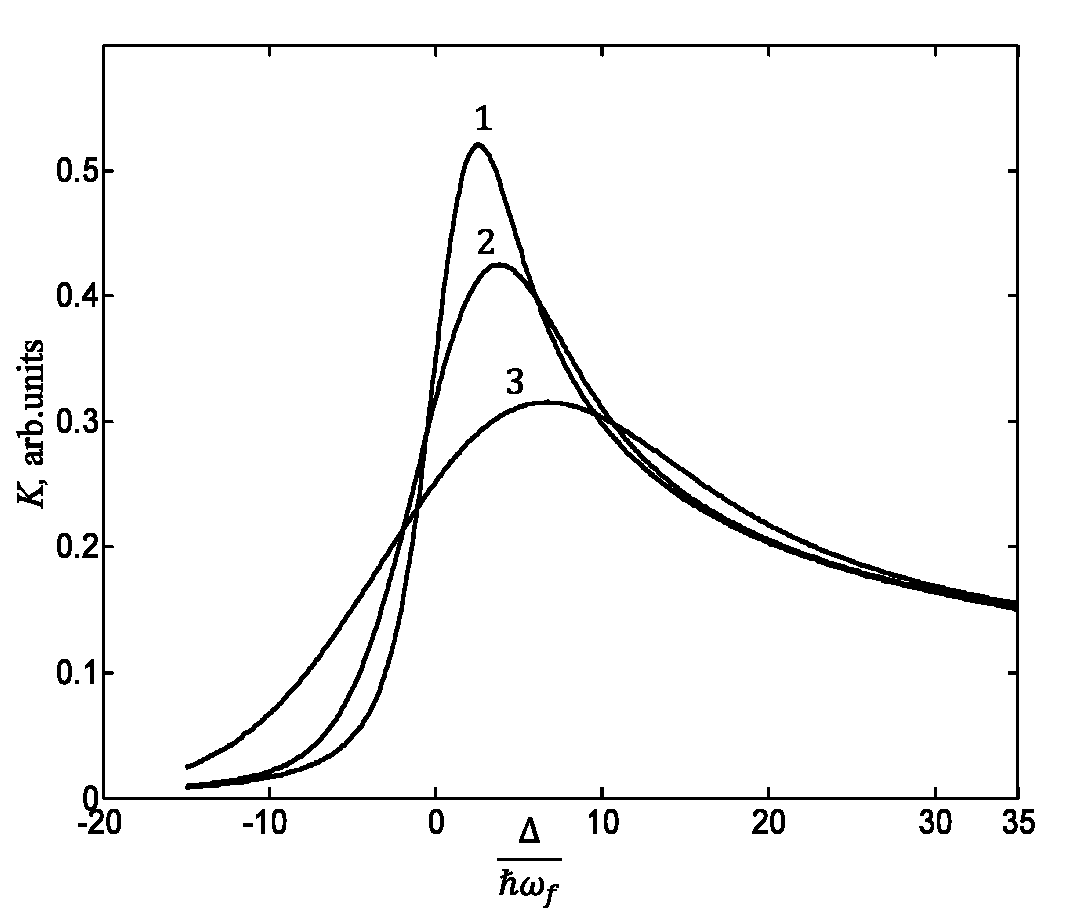
\includegraphics [scale=0.8] {fig_2_3_2}
	\caption{Зависимость первого пика межзонного поглощения света (в относительных единицах) от ${\Delta }/{\hbar {\omega }_f}$. Кривые 1, 2, 3 вычислены для $\xi =0.25,\; 0.05,\; 0.01$ соответсвенно.} 
	\label{img:fig_2_3_2} 
\end{figure}

На рисунке~\ref{img:fig_2_3_2} представлена частотная зависимость коэффициента поглощения света (в относительных единицах) при различных значениях интенсивности лазерного излучения. Кривые 1, 2, 3 получены соответственно при $\xi =0.25,\ 0.05,\ 0.01$ $\left(\xi =\omega^2_f / 4a \right)$. Как следует из рисунка~\ref{img:fig_2_3_2}, с ростом интенсивности ИК излучения ($\xi $ уменьшается при фиксированном значении $\omega_f$) форма линии поглощения изменяется: величина максимума поглощения уменьшается, а полуширина увеличивается. Заметим, что уже при $\xi \le 1$ коэффициент межзонного поглощения света полностью определяется интенсивностью ИК лазерного излучения.

Рассмотрим межзонное поглощение света в области второго пика магнетопоглощения (оптический переход II на рисунке~\ref{img:fig_2_3_1}) при $\omega_L=\Omega_e$ (магнито-инфракрасный резонанс). В этом случае коэффициент поглощения света согласно \eqref{eq:23_30} при $m=0$, $n=1$ $\left( L_1\left(2at^2\right)=1-2at^2 \right) $ принимает следующий вид:
\begin{multline} \label{eq:23_70}
K\left(\Omega\right)=K_0 {\left|\left\langle \widetilde{\alpha }_c |\widetilde{\alpha }_v\right\rangle \right|}^2 4{\left[\frac{2{\mu }^*{\omega }_f}{\hbar a}\right]}^{\frac{1}{2}}\times\\
\times Re\int\limits^{\infty }_0 {dx} f(x)\left\{-\sqrt{\pi }f\left(x\right)e^{f^2\left(x\right)}\left[1-\Phi \left(f\left(x\right)\right)\right]+1\right\}
\end{multline} 
 
При $\xi ={{\omega }^2_f}/{4a}\gg 1$ (лазерное излучение отсутствует) из \eqref{eq:23_70} следует выражение для коэффициента поглощения слабой электромагнитной волны, полученное в \cite{Kostyukevich2015}. При $\xi <1$ (форма линии поглощения определяется интенсивностью резонансного ИК излучения) получено:
\begin{multline} \label{eq:23_80}
K\left(\Omega\right)=K_0{\left|\left\langle \widetilde{\alpha }_c |\widetilde{\alpha }_v\right\rangle \right|}^2 \pi z{\left[\frac{2^* \pi }{\hbar }{\left(\frac{8z}{a}\right)}^{1/2}\right]}^{1/2}e^{-z}\times\\
\times \left\{-\left[I_{3/4}\left(z\right)+\mathrm{sign}(\Delta) I_{-3/4}\left(z\right)\right]+\left(1+\frac{1}{4z}\right)\left[(I_{-1/4}\left(z\right)+ \mathrm{sign}(\Delta)  I_{1/4}\left(z\right)\right]\right\}
\end{multline}
\[
\mathrm{sign}(\Delta) = \begin{cases}
1,&\Delta >0 \\ 
-1,&\Delta <0
\end{cases}
\] 
$\left\langle \widetilde{\alpha }_c |\widetilde{\alpha }_v \right\rangle$ --- матричный элемент сглаженных волновых функций носителей в возбужденном состоянии валентной зоны ($m=0$, $n=1$) и в первом возбужденном состоянии размерно-квантованной зоны проводимости.

\begin{figure}[!h] 
	\center
	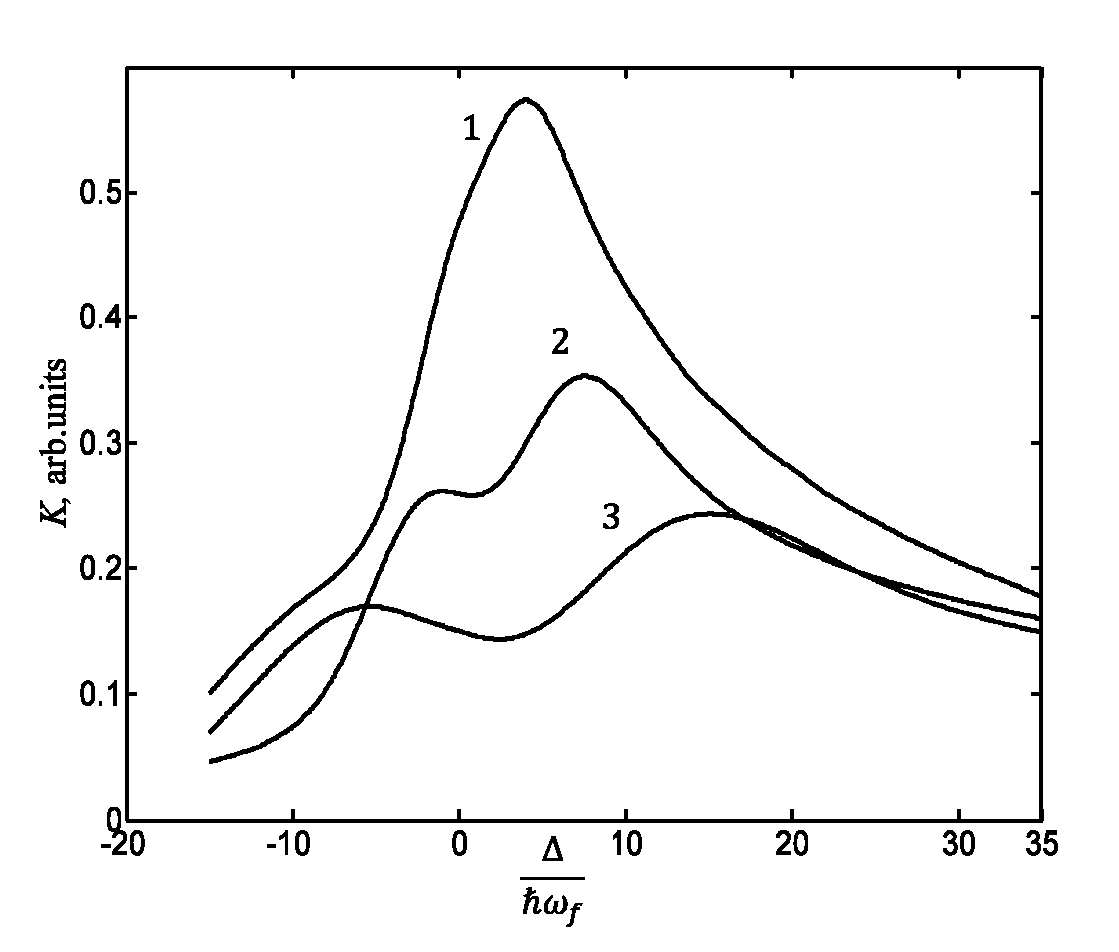
\includegraphics [scale=0.8] {fig_2_3_3}
	\caption{Зависимость второго пика магнетопоглощения (в относительных единицах) от ${\Delta }/{\hbar {\omega }_f}$ при различных значениях интенсивности резонансного $\left({\omega }_L=\Omega_e\right)$ лазерного излучения. Кривые 1, 2, 3 вычислены для $\xi=0.25,\; 0.05,\; 0.01$ соответсвенно.} 
	\label{img:fig_2_3_3} 
\end{figure}

На рисунке~\ref{img:fig_2_3_3} приведена частотная зависимость второго пика магнетопоглощения при различных значениях $\xi $. Кривые 1, 2, 3 вычислены при $\xi =0.25,\ \ 0.05,\ \ 0.01$ соответсвенно. Как следует из рисунка с ростом напряженности $E$ электрического поля пик магнетопоглощения деформируется и при $\xi \ll 1$ расщепляется на два пика. При этом расстояние между ними и их полуширина увеличивается. Расщепление второго пика поглощения связано с тем, что при $\omega_L=\Omega_e$ возбужденное гибридное состояние $(n=1)$ двукратно вырождено, и при взаимодействии с ИК лазерным излучением оно расщепляется. Эта ситуация близка к двойному оптическому резонансу (ДОР) на межзонных переходах в объемных материалах \cite{Perlin1970}.

Заметим, что $n$-пик магнетопоглощения расщепляется на $n$ пиков. Если рассматривать случай $z$-поляризованной электромагнитной волны лазерного излучения, когда $\omega_L=\omega_e$ (размерно-инфракрасный резонанс), то частотная зависимость коэффициента межзонного поглощения света (оптический переход III на рисунке~\ref{img:fig_2_3_1}) качественно не отличается от частотной зависимости, приведенной на рисунке~\ref{img:fig_2_3_2} и на рисунке~\ref{img:fig_2_3_3}.

Пусть при некотором значении напряженности электрического поля $E_c$ интенсивной электромагнитной волны вклад лазерного излучения в полуширину магнетоосцилляций примерно такой же как вклад, определяемый рассеянием носителей на шероховатой поверхности $(\xi =1)$. Естественно при $E_c<E$ форма линии межзонного поглощения слабой электромагнитной волны полностью определяется внешней лазерной подсветкой. Для типичных параметров полупроводниковой нанопроволоки $m_e=0.06m_0$, $m_v=0.4m_0$, $\sqrt[3]{\gamma_0}=20\ \AA $ (такое значение $\sqrt[3]{\gamma_0}$ хорошо описывает большие значения подвижности $\mu \propto 10^4\ \frac{cm^2}{V\cdot s}$, характерные для квантовых проволок) при $R_0=10^3\ \AA $, $E_c= 7\ \frac{V}{cm}$ для лазера $\mathrm{H_2 O}$ $\left(\hbar {\omega }_L=0.044\ eV\right)$. Следовательно, резонансное лазерное излучение заметно влияет на частотную зависимость межзонного поглощения света при небольших, вполне экспериментально доступных значений интенсивности ИК- лазерного излучения.
           % Глава 2
\chapter{Влияние шероховатой поверхности на кинетические эффекты в низкоразмерных системах} \label{chapt3}

\section{ Подвижность носителей в размерно-квантованных системах с учетом рассеяния на поверхности и фононах}

Квантовые системы с пониженной размерностью (квантовые ямы (КЯ), сверхрешетки, квантовые проволоки (КП)) благодаря их уникальным свойствам, связанных с возникновением размерного квантования, продолжают привлекать внимание теоретиков и экспериментаторов. При этом кинетические явления в размерно-квантованных системах принципиальным образом отличаются от объемных материалов. Так, например, в объемных материалах сопротивление растет с увеличением температуры $T$, а в КП малого диаметра $d$ ($d \sim 70 \AA$) убывает, оставаясь практически постоянным в области низких $T$ \cite{Lin2000,Lin2003,Heremans1998,Zhang2000,Heremans2000}. Для КЯ GaAs/AlAs температурная зависимость подвижности $\mu (T)$ может носить не монотонный характер: в области низких температур (T$>$10K) $\mu (T)$ увеличивается с ростом T, а при $T>100K$ начинает уменьшаться \cite{Lin2000,Sakaki1987}. Следовательно, размеры квантовых систем принципиальным образом могут влиять на величину и температурную зависимость электропроводности.

В данной главе делается попытка объяснить особенности температурной зависимости электропроводности, экспериментально наблюдаемые в нелегированных наноструктурах, учитывая процессы рассеяния носителей на шероховатой поверхности и на фононах. Именно из сравнения теоретических результатов с экспериментальными данными по температурной зависимости электропроводности можно провести оценки параметров флуктуирующей поверхности. Учет двух механизмов рассеяния позволил сформулировать условия на ширину размерно-ограниченной системы и температуру, когда рассеяние носителей на шероховатой поверхности преобладает над рассеянием на фононах.

Расчет электропроводности проводится согласно формуле Кубо \cite{Kubo1957a} для статической электропроводности, которая в представлении вторичного квантования имеет вид \footnote{ Полученное выражение для электропроводности справедливо для любых квантовых систем в произвольном магнитном поле. Единственное ограничение -- это малость электрического поля, т.е. область применимости закона Ома.}:
\begin{equation} \label{eq:31_10}
\sigma _{ij} =\frac{\beta_0 e^2 }{2 V m^2 } \sum _{\alpha,\beta, \alpha_1,\beta_1} \hat{p}_{\alpha \beta }^{(i)} \hat{p}_{\alpha_1 \beta }^{(j)} \int\limits_{-\infty }^{\infty} {dt\left\langle a_{\alpha }^+ (t) a_{\beta }(t) a_{\alpha_1 }^+ a_{\beta_1 } \right\rangle}
\end{equation} 
$\hat{p}_{\alpha \beta }^{(i)} $~---~матричный элемент оператора импульса на сглаженных волновых функциях зонного электрона, $\beta_0 = 1/k_0 T$, $\alpha $~---~квантовые числа, описывающие состояние заряженной частицы с эффективной массой $m_e$, $V$~---~объем основной области системы,
\[
a_{\alpha }^+ (t)= \exp\left(\frac{it\hat{H}}{\hbar } \right)a_{\alpha }^+ \exp\left(-\frac{it\hat{H}}{\hbar } \right),
\] 
$\left\langle \cdot \cdot \cdot \right\rangle $~---~описывает усреднение по системе равновесных электронов и по реализации случайного процесса.

Гамильтониан для электрона, взаимодействующего с шероховатой поверхностью размерно-ограниченной системы в представлении вторичного квантования записывается в виде:
\begin{equation} \label{eq:31_20}
\hat{H}=\sum _{\alpha }\varepsilon _{\alpha } a_{\alpha }^{+} a_{\alpha } +\sum _{\alpha ,\beta }{\left\langle \alpha  \right|} \hat{V}{\left| \beta  \right\rangle} a_{\alpha }^{+} a_{\beta }, 
\end{equation}
$\hat{V}$~---~оператор взаимодействия носителя с энергией $\varepsilon _{\alpha } $ с поверхностью системы, ${\left| \alpha  \right\rangle} $~---~волновая функция зонного электрона.

С гамильтонианом \eqref{eq:31_20} расчет временной зависимости операторов
рождения $a_\alpha ^ + (t)$ и уничтожения $a_\alpha (t)$ можно
провести точно по аналогии \cite{Khamidullin2002}. В результате
\begin{equation}
\begin{array}{c}\label{eq:31_23}
\displaystyle a_\alpha ^ + (t) = \exp\left(
{\frac{it\varepsilon _\alpha }{\hbar }} \right)\sum\limits_\beta
{a_\beta ^ + \left\langle \beta \right|} \exp\left[
{\frac{it}{\hbar }\left( {\hat {H}_0 + V} \right)}
\right]\exp\left( { - \frac{it}{\hbar }\hat {H}_0 }
\right)\left| \alpha \right\rangle ,\\
\displaystyle a_\alpha (t) = \exp\left( { - \frac{it\varepsilon
		_\alpha }{\hbar }} \right)\sum\limits_\beta {\left\langle \alpha
	\right|} \exp\left( {\frac{it}{\hbar }\hat {H}_0 }
\right)\exp\left[ { - \frac{it}{\hbar }\left( {\hat {H}_0 + V}
	\right)} \right]\left| \beta \right\rangle a_\beta .
\end{array},
\end{equation}
здесь обозначено: $\hat {H}_0 $ -- гамильтониан для свободных
носителей в координатном представлении $\left( \hat {H}_0 \left| \alpha
\right\rangle = \varepsilon _\alpha \left| \alpha \right\rangle
\right) $.

Если подставить \eqref{eq:31_23}  в \eqref{eq:31_10}, выражение для
электропроводности принимает следующий вид:
\begin{multline}
\sigma_{ij}=\frac{\beta_0e^2}{2Vm^2}\sum\limits_{\alpha	,\beta ,\alpha _1 ,\beta _1, \atop \gamma ,\gamma _1 } 
\hat{p}_{\alpha \beta}^{(i)} \hat {p}_{\alpha _1 \beta_1}^{(j)}
\int\limits_{- \infty }^\infty
{dt \left\{ \left\langle \gamma \left|\exp\left[\frac{it}{\hbar}\left(\hat{H}_0 + V\right)\right]\right|\alpha\right\rangle\right.}\times\\
\times\displaystyle\left.\left\langle \beta
\left|\exp\left[-\frac{it}{\hbar}\left(\hat {H}_0 +
V\right)\right]\right|\gamma_1\right\rangle\right\}_V \left\langle
{a_\alpha ^ + a_{\gamma _1 } a_{\alpha _1 }^ + a_{\beta _1 } }
\right\rangle _0,
\end{multline}
$\left\langle
{...} \right\rangle _0 $-- усреднение с равновесной матрицей
плотности для электронов.

Согласно теореме Вика:
\begin{equation} \label{eq:31_26}
\left\langle {a_\gamma ^ + a_{\gamma _1 } a_{\alpha _1
	}^ + a_{\beta _1 } } \right\rangle _0 = n_\gamma \left( {1 -
	n_{\gamma _1 } } \right)\delta _{\gamma \beta _1 } \delta _{\gamma
	_1 \alpha _1 } + n_\gamma n_{\alpha _1 } \delta _{\gamma \gamma _1
} \delta _{\alpha _1 \beta _1 } ,
\end{equation}
здесь
\begin{equation}  \label{eq:31_26_20}
n_\alpha = \frac{1}{\exp\left[ \beta \left( {\varepsilon _\alpha - \xi } \right) \right] + 1}
\end{equation}
равновесная функция распределения для электронов с энергией $\varepsilon{_\alpha}$, $\xi $~---~химический потенциал.

С учетом первого слагаемого \eqref{eq:31_26} тензор
электропроводности описывается соотношением:
\begin{multline}\label{eq:31_30}
\displaystyle\sigma_{ij}=\frac{\beta_0 e^2}{2Vm_e^2}
\sum\limits_{\alpha,\beta ,\beta_1 ,\alpha_1 } \hat {p}_{\alpha \beta}^{(i)} \hat{p}_{\alpha_1 \beta_1}^{(j)}
n_{\beta_1} \left( 1 - n_{\alpha_1}\right)\times\\
\times\int\limits_{- \infty }^\infty {dt \left\{ \left\langle\beta_1 \left| \exp\left[\frac{it}{\hbar}\left(\hat{H}_0 + V\right)\right]	\right|\alpha\right\rangle \right.} \displaystyle\left.\left\langle \beta\right|\exp\left[-\frac{it}{\hbar}\left(\hat{H}_0 + V\right)\right] \left|\alpha_1\right\rangle\right\}_V
\end{multline}
${\left\{\cdots \right\}}_V$~---~описывает усреднение по реализации случайного процесса $\Delta \left(x,y\right)$.

В дальнейшем проведем усреднение для матричных элементов в \eqref{eq:31_30} независимо. Такое приближение соответствует приближению «времени релаксации» \cite{Khamidullin2002} и конечные результаты для кинетических коэффициентов будут вероятно отличаться от тех, которые получаются при использовании решения классического уравнения Больцмана. 

Рассмотрим функцию
\begin{multline} \label{eq:31_40}
y_{{\beta }_1\alpha }=\exp\left(-\frac{it}{\hbar }E_{\beta_1}\right){\left\{\left\langle {\beta }_1\left|\exp\left[ {\frac{it}{\hbar }\left( {\hat {H}_0 + V} \right)} \right]\right|\alpha \right\rangle \right\}}_V=\\
={\left\{\left\langle {\beta }_1\left|T{\exp_{[-]} \left[\frac{i}{\hbar }\int^{\infty }_0{V\left(\tau \right)d \tau }\right]\ }\right|\alpha \right\rangle \right\}}_V,
\end{multline}
здесь обозначено:
\[
T{\exp_{\left[-\right]} \left[\frac{i}{\hbar }\int\limits^{\infty }_0 {V\left(\tau \right)d \tau } \right]}
	=\exp\left( {-\frac{it}{\hbar }\hat {H}_0 }\right)\exp\left[ {\frac{it}{\hbar }\left( {\hat {H}_0 + V} \right)} \right],
\] 
\[
V(\tau ) = \exp\left( {\frac{i\tau \hat {H}_0 }{\hbar }}\right)
V\exp\left( { - \frac{i\tau \hat {H}_0 }{\hbar }} \right).
\]
Усреднение по реализации случайного процесса в \eqref{eq:31_40} проведем с использованием кумулянтного усреднения \cite{Kubo1957a}. Тогда, выражение \eqref{eq:31_40} с точностью до второй кумулянты принимает следующий вид:
\[
y_{{\beta }_1\alpha }\left(t\right)=\left\langle {\beta }_1\left|{\exp \left\{-\frac{1}{{\hbar }^2}\int\limits^t_0{d \tau \int\limits^{\tau }_0{d {\tau }_1{\left\{V\left({\tau }_1\right)V\left(\tau \right)\right\}}_V}}\right\}\ }\right|\alpha \right\rangle
\]
Не трудно показать, что
\begin{equation} \label{eq:31_60}
{\dot{y}}_{{\beta }_1\alpha }\left(t\right)=-\frac{1}{{\hbar }^2}\int^t_0{d \tau \sum_{\gamma }{\left\langle {\beta }_1\left|{\left\{V\left({\tau }_1\right)V\left(t\right)\right\}}_V\right|\gamma \right\rangle y_{\gamma \alpha }\left(t\right)}}
\end{equation} 
Дальнейшие расчеты проводятся в диагональном приближении, так как процессы рассеяния носителей на шероховатой поверхности являются упругими и происходят в основном в одной размерно-квантованной зоне проводимости. Решение дифференциального уравнения \eqref{eq:31_60} в диагональном приближении $\gamma ={\beta }_1$ с начальным условием $y_{{\beta }_1\alpha }\left(0\right)={\delta }_{{\beta }_1\alpha }$ записывается следующим образом:
\begin{equation} \label{eq:31_70}
y_{\beta_1\alpha }(t)=\exp \left\{-\frac{1}{{\hbar }^2}\int\limits_0^t{d \tau \int\limits_0^{\tau} {d \tau_1 \left\langle \beta_1 \left| {\left\{V\left(\tau \right)V\left({\tau }_1\right)\right\}}_V\right| \beta_1 \right\rangle}} \right\} \delta_{\beta_1\alpha}
\end{equation} 
Не трудно показать, что
\begin{equation} \label{eq:31_80}
\left\langle \beta_1 \left| {\left\{V\left(\tau \right)V\left({\tau }_1\right)\right\}}_V\right| \beta_1 \right\rangle =\sum_{\gamma} {W_{\beta_1\gamma} \exp \left[\frac{i}{\hbar} \left(\tau_1-\tau \right) \left(\varepsilon_{\beta_1} - \varepsilon_{\gamma} \right)\right]\ }
\end{equation}
\begin{equation} \label{eq:31_85}
W_{\alpha\beta}=\int{d\vect{r} d\vect{r_1} \Psi^*_\alpha(\vect{r}) \Psi^*_\beta(\vect{r_1}) V_\alpha V_\beta F \Psi_\alpha(\vect{r_1}) \Psi_\beta(\vect{r})}
\end{equation}
Если подставить \eqref{eq:31_80} в \eqref{eq:31_70} и провести интегрирование по $\tau, \tau_1$, то в результате получаем
\begin{equation} \label{eq:31_90}
y_{\beta_1\alpha}(t)= \exp \left[g_{\alpha }\left(t\right)\right] \delta_{\beta_1\alpha}
\end{equation}
\begin{multline} \label{eq:31_100}
g_{\alpha}(t)=-2\sum_{\gamma}{W_{\alpha \gamma }\frac{\sin^2 \frac{t}{\hbar} (\varepsilon_{\alpha} - \varepsilon_{\gamma})}{{(\varepsilon_{\alpha} - \varepsilon_{\gamma})}^2}}+\\
+i\sum_{\gamma }{\frac{W_{\alpha \gamma}}{(\varepsilon_{\alpha} - \varepsilon_{\gamma})}}\left\{\frac{t}{\hbar }-\frac{1}{(\varepsilon_{\alpha} - \varepsilon_{\gamma})}{\sin\left[ \frac{t}{\hbar }(\varepsilon_{\alpha } - \varepsilon_{\gamma})\right] }\right\}.	
\end{multline}
Первое слагаемое в $g_{\alpha}\left(t\right)$ связано с квантово-механической вероятностью перехода носителя в единицу времени под влиянием возмущения $V$. Второе слагаемое, в частности, определяет сдвиг энергии электрона под влиянием возмущения $V$.
Подставляя \eqref{eq:31_90} в \eqref{eq:31_30}, электропроводность можно записать в виде:
\begin{multline} \label{eq:31_110}
\sigma_{ij}=\frac{\beta_0 e^2}{2V m^2_e}\sum_{\alpha\beta } {{\hat{P}}^{(i)}_{\alpha\beta} {\hat{P}}^{(j)}_{\beta\alpha} n_{\alpha} \left(1-n_{\beta}\right)} \times\\
\times \int\limits_{-\infty }^\infty {dt \exp{ \left[\frac{it}{\hbar} \left( \varepsilon_{\alpha } - \varepsilon_{\beta} \right) \right] }  \exp{ \left[ g_{\alpha }(t)+g_{\beta }(t)\right]} }.
\end{multline} 

Если рассматривать упругое рассеяние в одной зоне и учесть, что в дальнейшем исследуются кинетические процессы с $\hat{P}^{(i)}_{\alpha \beta }\sim {\delta }_{\alpha \beta }$, то \eqref{eq:31_110} можно представить в виде $(i=j)$:
\begin{multline} \label{eq:31_120}
\sigma_{ii}=\frac{{\beta }_0e^2}{2Vm^2_e}\sum_{\alpha }{{\left|{\hat{P}}^{(i)}_{\alpha \alpha }\right|}^2 n_{\alpha }\left(1-n_{\alpha }\right)}\times\\
\times\int\limits_{- \infty }^\infty {dt \exp \left[-\sum_{\gamma }{W_{\alpha \gamma }\frac{4 \sin^2 \frac{t}{\hbar}\left({\varepsilon }_{\alpha }-{\varepsilon }_{\gamma }\right)}{(\varepsilon_{\alpha } - \varepsilon_{\gamma })^2}}\right]}
\end{multline}

При $t\to \infty $, когда можно ввести понятие о независящей от времени вероятности перехода \cite{LandauT3}, тогда
\begin{equation} \label{eq:31_130}
\sum_{\gamma }{W_{\alpha \gamma }\frac{4 \sin^2 \frac{t}{\hbar}\left(\varepsilon_{\alpha } - \varepsilon_{\gamma }\right)}{(\varepsilon_{\alpha } - \varepsilon_{\gamma })^2}} \Rightarrow \left|t\right|\frac{1}{\tau_{\alpha}};
\end{equation}
\begin{equation} \label{eq:31_140}
\frac{1}{\tau_{\alpha}}=\frac{2\pi}{\hbar} \sum_{\gamma} {W_{\alpha\gamma} \delta \left(\varepsilon_{\alpha} - \varepsilon_{\gamma} \right)}
\end{equation}
${1}/{\tau_{\alpha}}$~---~квантово-механическая вероятность рассеяния носителей в единицу времени на шероховатой поверхности.

С учетом \eqref{eq:31_130} электропроводность определяется соотношением
\begin{equation} \label{eq:31_150}
\sigma_{ij}=\frac{\beta_0e^2}{Vm^2_e}\sum_{\alpha }{\left|{\hat{P}}^{(i)}_{\alpha \alpha }\right|}^2n_{\alpha }\left(1-n_{\alpha }\right)\tau_{\alpha }
\end{equation}

Заметим, что соотношение для электропроводности \eqref{eq:31_150} получено из самых общих соотношений квантовой статистики без привлечения решения классического уравнения Больцмана, которое, как известно, имеет ограниченную область применения. В классическое выражение для тензора электропроводности входит не время релаксации ${\tau }_{\alpha }$, а транспортное время релаксации, которое естественным образом возникает при решении кинетического уравнения Больцмана \cite{Anselm1978}. При этом время релаксации и транспортное время в случае упругого рассеяния носителей на длинноволновых акустических колебаниях, на примесях, при рассеянии на шероховатой поверхности в случае $\delta $-образной флуктуации поверхности не отличаются (в случае гауссовой флуктуации поверхности см. замечание в \ref{sect1_2}). Последнее обстоятельство является не случайным, т.к. выражение для электропроводности \eqref{eq:31_150} получено при условии упругих процессов рассеяния носителей и при возможности введения независимой от времени вероятности процесса рассеяния. Но именно из тех же соображений вводится интеграл столкновений при выводе классического уравнения Больцмана.

Рассмотрим прямоугольную КЯ с бесконечным потенциалом с гауссовой флуктуацией поверхности. В этом случае время релаксации при рассеянии носителей в одной зоне определяется соотношением \eqref{eq:1_9}. При низких температурах  $3\hbar^2 \pi^2 /\left(2m_e L^2 \right) \gg k_0 T$ когда электроны находятся на нижайшем размерно-квантованном уровне $(n=1)$ прямоугольной КЯ выражение \eqref{eq:31_150} после суммирования по $k_{\bot } $ принимает вид $(i=x)$:
\begin{equation} \label{eq:31_180}
\sigma _{xx} =\frac{e^2 \hbar^3 \delta}{m_e^2 \pi^2 \left(\Delta \Lambda^2 V_1 \right)^2 L} \int\limits_0^\infty { \frac{d\tau \cdot \tau \cdot \exp \left(\delta \tau -\beta_0 \tilde{\xi }\right)}{\exp(-\tau )\mathrm{I}_0 (\tau )\cdot \left[\exp \left(\delta \tau -\beta_0 \tilde{\xi }\right)+1\right]^2 }},
\end{equation}
\[
\beta_0 = \frac{1}{k_0 T}, \; \delta =\frac{\beta_0 \hbar^2 }{m_e \Lambda^2 },
\] 
$\tilde{\xi }=\xi -\varepsilon _{1} $ --- химический потенциал, отсчитанный от дна нижайшей зоны проводимости,
\begin{equation} \label{eq:31_190}
\beta_0 \tilde{\xi }=\ln\left[\exp\left(\frac{\beta_0 \pi \hbar^2 n_s }{m_e} \right)-1\right].
\end{equation}
$n_s $~---~поверхностная плотность электронного газа.

Для невырожденного электронного газа $(\beta_0 \pi \hbar^2 n_s /m_e \ll 1)$
$$\exp(\beta_0 \tilde{\xi }) = \frac{\beta_0 \pi \hbar^2 n_s}{m_e} $$
и согласно \eqref{eq:31_180} подвижность определяется соотношением:
\begin{equation} \label{eq:31_200}
\mu ^{(nd)} =\mu _{0} \delta^2 \int\limits_0^\infty {d\tau \frac{\tau \cdot \exp \left[-\left(\delta -1\right)\tau \right]}{\mathrm{I}_0 (\tau )}},
\end{equation}
\[
\mu _{0} =\frac{e}{\hbar \pi^5 } \left(\frac{L^3 }{\Delta \Lambda } \right)^2.
\] 

\begin{figure}[!h]
	\center
	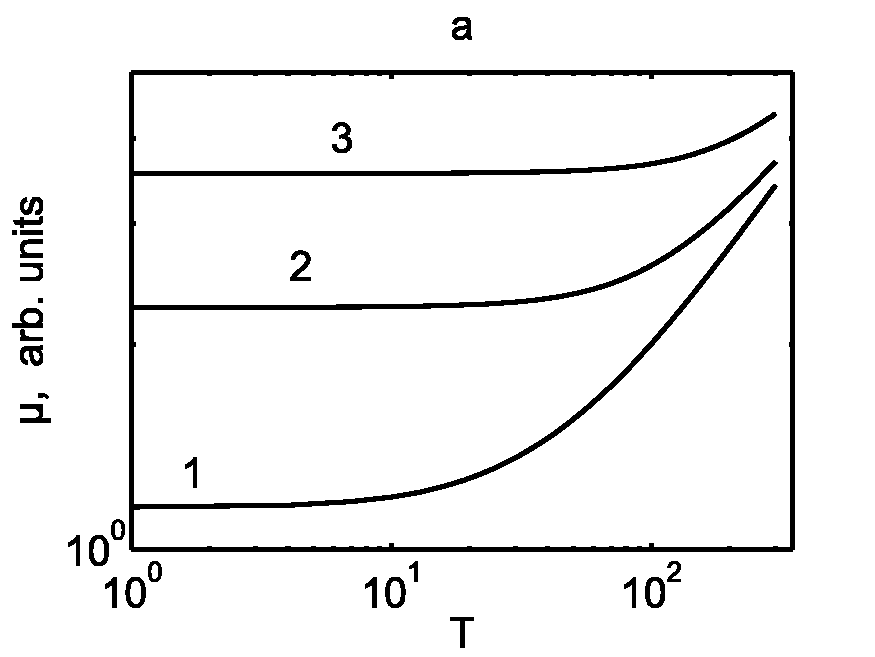
\includegraphics [scale=1] {fig_3_1_1}
	\caption{Температурная зависимость подвижности (в относительных единицах) при учете рассеяния носителей на шероховатой поверхности в КЯ при $\Lambda =70 \AA$, $\Delta =3 \AA$, $L_0 = 100 \AA$, кривые 1, 2, 3 получены соответственно для $n_s = 10^{11} \text{cm}^{-2}$, $n_s = 7 \cdot 10^{11} \text{cm}^{-2}$, $n_s = 1.5 \cdot 10^{12} \text{cm}^{-2}$.}
	\label{img:fig_3_1_1} 
\end{figure}

Следовательно, подвижность существенным образом зависит от толщины размерно-квантованной системы $(\mu_0 \sim L^6 )$. На рисунке~\ref{img:fig_3_1_1} (кривая 1) приведена температурная зависимость $\mu ^{(nd)} /\mu_0 $ с учетом зависимости химического потенциала от температуры \eqref{eq:31_190}. Как непосредственно следует из рисунка~\ref{img:fig_3_1_1}, при низких $T$ $(\delta \gg 1)$ подвижность практически не зависит от температуры и при высоких температурах $(\delta <1)$ с ростом $T$ увеличивается (кривая 1). Такое поведение подвижности от $L$ и $T$ экспериментально наблюдалось в GaAs/AlAs \cite{Sakaki1987}. При низких температурах $\mu ^{(nd)} =\mu_0 $, т.е. определяется только размером КЯ и параметрами флуктуирующей поверхности $\Delta $, $\Lambda $. При изменении толщины КЯ от $70 \AA$ до $100 \AA$ подвижность изменяется от $\mu_0 =2.6\cdot 10^3 \text{cm}^2 / \text{Vs}$ до $\mu_0 =2\cdot 10^4 \text{cm}^2 /\text{Vs}$, что согласуется с экспериментальными данными в КЯ GaAs/AlAs \cite{Sakaki1987}.

Для вырожденного электронного газа при низких $T$ электропроводность принимает вид:
\begin{equation} \label{eq:31_210}
\sigma _{xx}^{(d)} =\frac{e^2 \hbar \tilde{\xi }}{\pi^2 L m_e \left(\Delta \Lambda V_{1} \right)^2 } \frac{\exp{\left(\frac{m_e \Lambda^2 }{\hbar^2 } \tilde{\xi }\right)}}{\mathrm{I}_0 \left(\frac{m_e \Lambda^2 }{\hbar^2 } \tilde{\xi }\right)}.
\end{equation}
Если $\beta_0 \pi \hbar^2 n_s /m_e \gg 1$, то $\tilde{\xi }=\pi \hbar^2 n_s /m_e$ и подвижность определяется соотношением:
\begin{equation} \label{eq:31_220}
\mu^{(d)} =\mu _{0} \frac{\exp (a)}{\mathrm{I}_0 (a)},
\end{equation}
\[
a=\pi \Lambda ^{2} n_{s}
\]
При $a \ll 1 \; (\mathrm{I}_0 (a) \simeq 1)$ 
\begin{equation} \label{eq:31_230}     
\mu ^{(d)} =\mu _{0}.
\end{equation}
При $a \gg 1  \; (\mathrm{I}_0 (a) \simeq e^a / \sqrt{2\pi a})$
\begin{equation} \label{eq:31_240}  
\mu ^{(d)} =\mu _{0} \pi \sqrt{2\Lambda ^{2} n_{s} }
\end{equation}

Как следует из \eqref{eq:31_230} в исследуемой модели КЯ подвижность в области низких температур не зависит от $T$ (кривая 2 на рисунке~\ref{img:fig_3_1_1}). Такое поведение $\mu^{(d)} $ от $T$ экспериментально наблюдалось в кремниевых инверсионных слоях, в которых электронный газ остается вырожденным вплоть до $T<100 K$ ($\tilde{\xi }=12.5 \text{meV}$, $n_{s} =2\cdot 10^{12} \text{cm}^{-2} $) \cite{Stern1980}. Для $\Delta =6\AA$, $\Lambda =13 \AA$, при $L=70 \AA$, $n_{s} =2\cdot 10^{12}  \text{cm}^{-2} $ $(a \ll 1)$ $\mu^d =1.5 \cdot 10^4 \text{cm}^2 /\text{Vs}$, что близко к экспериментальным данным \cite{Stern1980}.

Аналогичные расчеты подвижности можно провести для прямоугольной квантовой ямы при $\delta$-образной флуктуации поверхности. Учитывая предельный переход от гауссовой флуктуации поверхности к $\delta $-образной, когда $\Lambda \to 0$, ${\left(\Delta \Lambda \right)}^2\to \pi \gamma $ (см. замечание в \ref{sect1_2}) можно получить выражение для электропроводности. Согласно \eqref{eq:31_180} электропроводность в этом случае может быть записана в виде:

\begin{equation} \label{eq:31_250}
{\sigma }^{\delta }_{xx}=\frac{e^2\hbar }{{\pi }^3{\beta }_0 m_e L V^2_0 \gamma_0 }\int\limits_0^\infty{\frac{x dx \exp{(x-\beta \widetilde{\xi })}}{{\left[ \exp{(x-\beta \widetilde{\xi })}+1 \right] }^2}}
\end{equation}
Из \eqref{eq:31_250} не трудно получить выражения для подвижности вырожденного и невырожденного электронного газа: 
\begin{equation} \label{eq:31_260}
\mu^{\delta \left(d\right)} = \mu^{\delta \left(n d\right)}=\frac{e L^6}{\hbar {\pi }^6\gamma },
\end{equation}
которые совпадают и существенным образом зависит от размеров квантовой системы и не зависят от температуры

Для КП потенциал взаимодействия носителей с шероховатой поверхностью определяется \eqref{eq:1_1} и в случае гауссовской флуктуации поверхности автокорреляционная функция для различных точек поверхности записывается в виде \eqref{eq:1_6}. С учетом волновых функций для квантовой проволоки \cite{Constantinou1989} $W_{\gamma \alpha } $ легко вычисляется и $\tau_{\alpha }^{-1} $ принимает следующий вид:
\begin{equation} \label{eq:31_290}
\frac{1}{\tau _{\alpha } } =\frac{(\Delta \tilde{V}_0 )^2 m\Lambda \sqrt{\pi } }{\hbar^3 \left|k_x \right|} \left\{1+ \exp\left[-\left(k_x \Lambda \right)^2 \right]\right\}.
\end{equation}
Подставляя \eqref{eq:31_290} в \eqref{eq:31_150} и интегрируя по квазиимпульсу электрона $\hbar k_x $ нетрудно получить:
\begin{equation} \label{eq:31_300}
\sigma_{xx} =\frac{2 e^2 \hbar^3 \delta }{m^2 \pi^2 \sqrt{\pi } R_0^2 (\Delta \Lambda \tilde{V}_1 )^2 \Lambda } \int \limits_0^{\infty }{d\tau \frac{\tau \cdot \exp(\delta \tau -\beta_0 \tilde{\xi })}{\left[ \exp(-\tau )+1\right] \cdot \left[ \exp(\delta \tau -\beta_0 \tilde{\xi })+1\right]^2 }},
\end{equation}
$\beta_0 \tilde{\xi }$ определяется из уравнения:
\[
\sum_{\alpha } {f_{\alpha}(\tilde{\xi }) = N},
\]
которое приводится к виду:
\begin{equation} \label{eq:31_305}
\int\limits_0^{\infty }{\frac{dx}{\exp \left(x^2 -\beta_0 \tilde{\xi }\right)+1}} =\frac{n_l \pi \hbar \sqrt{\beta_0 } }{\sqrt{8m} },
\end{equation}
$n_{l} =N/L_{x} $ -- линейная плотность электронов.

\begin{figure}[!h]  
	\center
	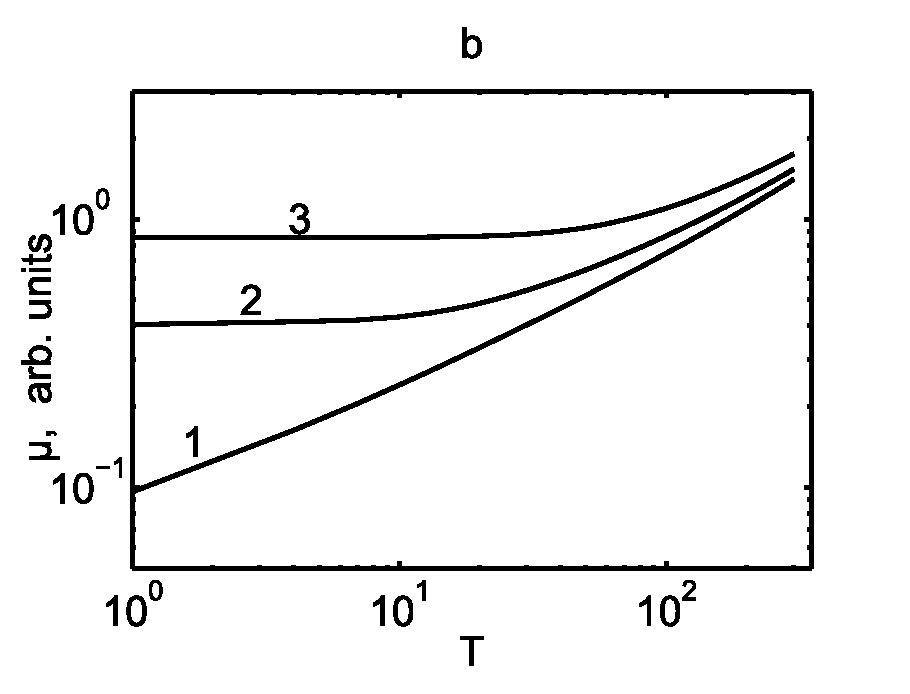
\includegraphics [scale=1] {fig_3_1_2}
	\caption{Температурная зависимость подвижности (в относительных единицах) при учете рассеяния носителей на шероховатой поверхности в КП при $\Lambda =20 \AA$, $\Delta =2 \AA$, $R_0=100 \AA$, кривые 1, 2, 3 получены соответственно для $n_l = 10^5 \text{cm}^{-1}$, $n_l = 5 \cdot 10^5 \text{cm}^{-1}$, $n_s = 10^6 \text{cm}^{-1}$.}
	\label{img:fig_3_1_2}	
\end{figure}

На рисунке~\ref{img:fig_3_1_2} представлена температурная зависимость электропроводности (в относительных единицах) в КП с учетом зависимости химического потенциала от концентрации носителей и температуры \eqref{eq:31_305}. Для невырожденного электронного газа (кривая 1 на рисунке~\ref{img:fig_3_1_2}) электропроводность описывается корневой зависимостью от температуры ($\sigma_{xx}^{(nd)} \sim \sqrt{T} $).

Для вырожденного электронного газа искомая электропроводность (рассматривается нижайшая электронная зона) записывается в следующем виде:
\begin{equation} \label{eq:31_310}
\sigma _{xx}^{(d)} =\frac{4 e^2 \hbar \tilde{\xi }}{\pi^2 \sqrt{\pi } R_0^2 m \left(\Delta \tilde{V}_1 \right)^2 \Lambda } \cdot \frac{1}{1+{\exp}(-q)} , q=\frac{2m\Lambda^2 }{\hbar^2 } \tilde{\xi }.  
\end{equation}

Как непосредственно следует из \eqref{eq:31_310}, для вырожденных КП электропроводность, а следовательно и подвижность, при низких температурах не зависит от T (кривая 3 на рисунке~\ref{img:fig_3_1_2}). Такое поведение электропроводности от температуры экспериментально наблюдалось в КП Bi \cite{Lin2000,Heremans1998,Zhang2000,Heremans2000,Gitsu2003,Nikolaeva2006,Gitsu2005}.

Из рисунков~\ref{img:fig_3_1_1}-\ref{img:fig_3_1_2} следует, что электропроводность при рассеянии носителей на шероховатой поверхности размерно-квантованной системы в области низких температур слабо (для невырожденных квантовых систем) или вообще не зависит (для вырожденного электронного газа) от T. При этом с ростом T $\sigma _{xx} $, а следовательно и подвижность, начинает увеличиваться. Однако как показывают экспериментальные исследования \cite{Zhang2000,Gitsu2003,Nikolaeva2006} при высоких температурах подвижность уменьшается. Следовательно «включается» другой механизм рассеяния носителей, например, на колебаниях решетки. Поэтому для последовательного сравнения теории с экспериментом рассмотрим температурную зависимость электропроводности с учетом двух механизмов рассеяния (на шероховатой поверхности и на фононах). Это обстоятельство позволяет исследовать поведение подвижности в широкой области температур ($T\le 200\text{K}$).

В приближении времени релаксации, если использовать соотношение \eqref{eq:31_120} и результаты работы \cite{Khamidullin2002} выражение для электропроводности записывается следующим образом

\begin{equation} \label{eq:31_320}
\sigma _{xx} =\frac{\beta_0 e^2 }{Vm^2 } \sum _{\alpha }\left|\hat{p}_{\alpha \alpha }^{(x)} \right|^2 \frac{\tau _{\alpha } \tau_{\alpha }^f }{\tau_{\alpha } +\tau_{\alpha }^f } n_{\alpha } \left(1-n_{\alpha } \right),
\end{equation}
$\tau _{\alpha } $ --- время релаксации, определяемое рассеянием электронов на шероховатой поверхности, $\tau_{\alpha }^f $ --- время релаксации, связанное с рассеянием электрона на фононах \cite{Khamidullin2002}.

Для прямоугольной КЯ при рассеянии электронов в нижайшей зоне проводимости:
\begin{equation} \label{eq:31_330}
\frac{1}{\tau_{\alpha }^f } = \frac{3 E_1^2 m}{\beta_0 \hbar^3 \rho \nu^2 L},
\end{equation}
здесь $E_1 $ -- константа деформационного потенциала для электрона, $\nu $ -- скорость звука в кристалле с плотностью $\rho $.

Для КП с бесконечным потенциалом для нижайшей зоны проводимости:
\begin{equation} \label{eq:31_340}
\frac{1}{\tau _{\alpha }^f } =\gamma_f \frac{1}{\left|k_{x} \right|}, \;
\gamma_f =\frac{4 E_1^2 m}{\beta_0 \hbar^3 \rho \nu^2 \pi R_0^2 },
\end{equation}
выражение для электропроводности прямоугольной КЯ записывается в виде:
\begin{multline} \label{eq:31_350}
\sigma _{xx} =\frac{e^2 \hbar^3 }{\pi^2 m^2 \left(\Delta \Lambda^2 V_1 \right)^2 L} \delta^2 \gamma \times \\
 \times \int\limits_0^{\infty }{d\tau \frac{\tau \cdot \exp (\delta \tau -\beta \tilde{\xi })}{\left[\delta \gamma \cdot \exp(-\tau ) \mathrm{I}_0 (\tau )+1\right]\cdot \left[\exp(\delta \tau -\beta \tilde{\xi })+1\right]^2 }},
\end{multline}
\[
\delta =\frac{\hbar^2 \beta_0 }{m \Lambda^2 }, \;
\gamma =\frac{\pi m\rho \nu^2 L}{3\hbar^2 E_1^2 } \left(\Delta \Lambda^2 V_1 \right)^2 .
\]
 
Для невырожденного электронного газа подвижность определяется соотношением:
\begin{equation} \label{eq:31_360}
\mu ^{(nd)} =\mu_0 \cdot \delta^3 \gamma \int\limits_0^{\infty}{d\tau \frac{\tau \cdot \exp(-\tau \delta )}{\delta \gamma \cdot \exp(-\tau ) \mathrm{I}_0 (\tau )+1}}. 
\end{equation}

Если $\delta \gamma \ll 1$, то из \eqref{eq:31_360} получается выражение для подвижности, связанное с рассеянием носителей на длинноволновых колебаниях:

\begin{equation} \label{eq:31_370}
\mu _{xx}^{(fnd)} =\frac{e\hbar^3 \rho \nu^2 L^2 }{3m_e^{2} E_1^2 } \beta_0. 
\end{equation}

Для типичных параметров КЯ GaAs/AlAs ($\rho =5.4 \text{ g} / \text{cm}^3 $, $v=5\cdot 10^5 \text{ cm/s}$, $E_1 =7 \text{ eV}$, $m_e=0.06m_0 $) при $\Delta =3 \AA$, $\Lambda =70 \AA$, $L = 100 \AA$  $\gamma \delta \cong 520/\text{T}$ и, следовательно, при $T>100\text{ K}$ рассеяние носителей на фононах начинает заметно влиять на температурную зависимость подвижности.

Для случая вырожденного электронного газа:
\begin{equation} \label{eq:31_380}
\sigma _{xx}^{(d)} =\frac{e^2 \hbar^3 }{\pi^2 m^2 \left(\Delta \Lambda^2 V_0 \right)^2 L} \cdot 
\frac{\delta \gamma \cdot \delta_0 }{\delta \gamma \cdot \mathrm{I}_0 \left(\delta_0 \right)\exp\left(-\delta_0 \right)+1} ,
\end{equation}
$n_s $~---~поверхностная плотность электронов, $\delta_0 =\pi \Lambda^2 n_s $.

При $\delta \gamma \gg 1$ из \eqref{eq:31_380} получается выражение для подвижности \eqref{eq:31_220}. Если $\delta \gamma \ll 1$, то из \eqref{eq:31_380} следует соотношение для подвижности в прямоугольной квантовой яме, когда учитывается взаимодействие носителей с длинноволновыми фононами:
\begin{equation} \label{eq:31_390}
\mu _{xx}^{(fd)} =\frac{e\hbar^3 \rho \nu^2 L\beta_0 }{3 m^2 E_1^2 }. 
\end{equation}
 
Аналогичным образом можно вычислить электропроводность для квантовых проволок с параболическим потенциалом, используя соотношения \eqref{eq:31_300}, \eqref{eq:31_340}:
\begin{multline} \label{eq:31_400}
\sigma _{xx} =\frac{2e^2 \hbar^3 \delta^2 q}{m^2 \pi^2 \sqrt{\pi } R_0^2 \left(\Delta \Lambda V_1 \right)^2 \Lambda } \times\\
\times\int\limits_0^{\infty} {d\tau \frac{\tau \cdot {\exp}\left(\delta \tau -\beta _{0} \tilde{\xi }\right)}{\left[\delta q\cdot \left(\exp(-\tau) +1 \right)+1\right]\cdot \left[{\exp}\left(\delta \tau -\beta _{0} \tilde{\xi }\right)+1\right]^{2} }}, 
\end{multline}
\[
\delta =\frac{\beta_0 \hbar^2 }{2m\Lambda^2 }, \;
q=\frac{m \rho \nu^2 \sqrt{\pi } \pi R_0^2 }{2\hbar^2 E_1^2 } \left(\Delta \Lambda V_0 \right)^2 \Lambda .
\] 

Для невырожденного электронного газа квантовой проволоки \eqref{eq:31_400} принимает вид:
\begin{equation} \label{eq:31_410}
\sigma_{xx}^{(nd)} =\frac{2e^2 \hbar^3 n_e }{\pi m_e^2 \left(\Delta \Lambda V_0 \right)^2 } q \delta ^{\frac{5}{2} }
\int\limits_0^{\infty }{d\tau \frac{\tau \cdot \exp (-\delta \tau )}{\left[\delta q\cdot \left( \exp(-\tau )+1\right)+1\right]}}. 
\end{equation}

При $\delta q \ll 1$ из \eqref{eq:31_410} непосредственно следует выражение для электропроводности, связанное с рассеянием электронов на длинноволновых (акустических) фононах:
\begin{equation} \label{eq:31_420}
\sigma _{xx}^{(nd)} =\frac{e^2 \hbar^2 n_e R_0^2 \rho \nu^2 }{m E_1^2 } \sqrt{\frac{\beta_0 \pi }{2m_e} }
\end{equation}

Для вырожденного электронного газа:
\begin{equation} \label{eq:31_430}
\sigma _{xx}^{(d)} =\frac{2 e^2 \hbar^3 }{\pi^2 R_0^2 m_e^2 \sqrt{\pi } \left(\Delta \Lambda V_0 \right)^2 \Lambda } \cdot \frac{\delta q \cdot \delta_1 }{\delta q\cdot \left(1+{\exp}(-\delta_1 )\right)+1}, 
\end{equation}
\[
\delta_1 =\frac{2 m_e\Lambda^2 }{\hbar^2 } \tilde{\xi }. 
\]
Если $\delta q\gneq1$, то электропроводность имеет вид:
\begin{equation} \label{eq:31_440}
\sigma _{xx}^{(fnd)} =\frac{e^2 \hbar \rho \nu^2 \beta_0 }{\pi m E_1^2 } \tilde{\xi }.
\end{equation}

\begin{figure}[!h]  
	\center
	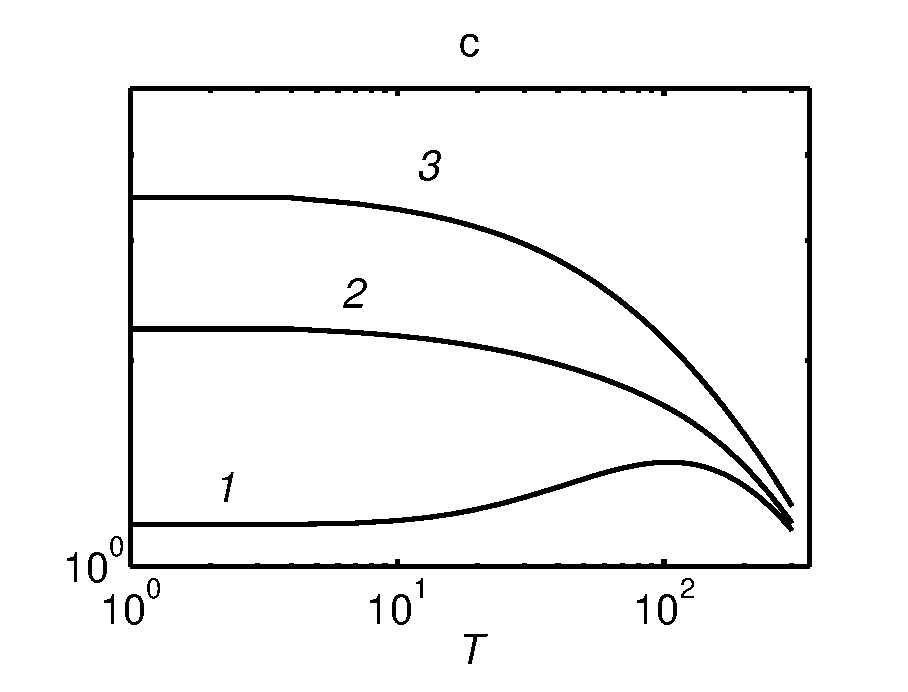
\includegraphics [scale=1] {fig_3_1_3}
	\caption{Температурная зависимость подвижности (в относительных единицах) при учете рассеяния носителей на шероховатой поверхности и на фононах в КЯ при $\Lambda =70 \AA$, $\Delta =3 \AA$, $L_{0}=100 \AA$, кривые 1, 2, 3 получены соответственно для $n_s = 10^{11} \text{cm}^{-2}$, $n_s = 7 \cdot 10^{11} \text{cm}^{-2}$, $n_s = 1.5 \cdot 10^{12} \text{cm}^{-2}$.} 
	\label{img:fig_3_1_3}	
\end{figure}

На рисунке~\ref{img:fig_3_1_3} приведена температурная зависимость подвижности (в относительных единицах) для различных концентраций носителей в прямоугольной КЯ. Для невырожденного электронного газа (кривая 1) подвижность немонотонным образом зависит от T, что экспериментально наблюдалось в КЯ GaAs/AlAs \cite{Sakaki1987}. Заметим, что с ростом ширины КЯ уменьшается влияние рассеяния носителей на шероховатости поверхности, поэтому максимум подвижности смещается в область низких температур. Кривые 2, 3 описывают температурную зависимость подвижности для вырожденного электронного газа. При низких T подвижность практически не зависит от температуры и с ее ростом уменьшается. Именно такое поведение подвижности от температуры экспериментально наблюдалось в инверсионных слоях Si для вырожденного электронного газа \cite{Stern1980}.

\section{ Электропроводность в размерно-квантовых системах с учётом рассеяния носителей на шероховатой поверхности в магнитном поле}

Рассмотрим особенности электропроводности, возникающие в в квантовых ямах в присутствии однородного магнитного поля напряжённостью $\vect{H}$. Волновые функции и собственные значения в таких системах известны \cite{Tavger1966} и имеют вид ($\vect{H} \parallel OX$, размерное квантование по $OZ$):
\begin{equation} \label{eq:32_05_10}
\Psi^{(c)}_{k_x,k_y,n}(x,y,z)=\frac{e^{ik_x x}}{\sqrt{L_x}}\frac{e^{ik_y y}}{\sqrt{L_y}}{\left(\frac{\lambda }{\pi }\right)}^{\frac{1}{4}}\frac{1}{\sqrt{2^n n!}}H_n\left[(z-z_0)\sqrt{\lambda }\right]e^{-\frac{\lambda }{2}(z-z_0)^2},
\end{equation}
\begin{equation} \label{eq:32_05_20}
E_{\alpha }=\frac{\hbar^2 k^2_x}{2m_e}+{\left(\frac{\omega }{\Omega }\right)}^2\frac{\hbar^2 k^2_y}{2m_e} +\hbar\Omega \left(n+\frac{1}{2}\right),
\end{equation}
здесь обозначено
\[
\lambda =\frac{m_e\Omega }{\hbar },\;
\Omega =\sqrt{\omega^2+\omega^2_c},\;
z^{(c)}_0=-\frac{\hbar \omega_c k_x}{m_e \Omega^2},
\]
$\hbar \omega =\dfrac{1}{L} \sqrt{\dfrac{8\Delta E_c }{m_e}} $~---~шаг пространственного квантования,
$\omega_c=\dfrac{eH}{m_e c}$~---~циклотронная частота.

Из \eqref{eq:32_05_20} следует, что выражение для $ V_{\alpha}$ в \eqref{eq:1_1} имеет вид:
\begin{equation} \label{eq:32_05_30}
V_{\alpha} = \frac{\partial E_{\alpha }}{\partial L}=\hbar \left[\frac{\hbar\omega}{m_e \Omega^2} {\left(\frac{\omega_c}{\Omega }\right)}^2 k^2_y+\frac{\omega}{\Omega} \left(n+\frac{1}{2}\right)\right] \frac{\partial\omega}{\partial L}.
\end{equation}
Первым слагаемым в \eqref{eq:32_05_30} можно пренебречь когда
\[
\frac{\hbar^2}{2m_e}k^2_y \ll \hbar \Omega.
\]
Последнее неравенство, как правило выполняется т.к. рассеяние на шероховатой поверхности вносит заметный вклад при низких температурах и заметном размерном квантовании. Тогда
\begin{equation} \label{eq:32_05_40}
V_{\alpha} = V_n = 2 V_0 \left(n+\frac{1}{2}\right),
\end{equation}
\begin{equation} \label{eq:32_05_42}
V_0 = \frac{\hbar}{2} \frac{\omega}{\Omega} \frac{\partial\omega}{\partial L}
\end{equation}
и для $\delta$-коррелированной поверхности матричный элемент взаимодействия \eqref{eq:31_85} при рассеянии в одной размерно-квантованной зоне равен:
\begin{equation} \label{eq:32_05_50}
W_{\alpha \beta }=\frac{\gamma_0 V^2_n}{L_x L_y} \delta_{\alpha \beta},
\end{equation}
следовательно время релаксации \eqref{eq:31_140} принимает вид:
\begin{equation} \label{eq:32_05_60}
\frac{1}{\tau_{\alpha }}=\frac{\gamma_0 m_e V_n^2}{\hbar^3}\left(\frac{\Omega }{\omega }\right).
\end{equation}

Для вычисления электропроводности вдоль магнитного поля $\sigma_{xx}$ необходим матричный элемент импульса $P^{(x)}_{\alpha\beta}$ на волновых функциях \eqref{eq:32_05_10}, который описывается соотношением \cite{Sinyavskii1998}:
\begin{equation} \label{eq:32_05_70}
P^{(x)}_{\alpha\beta} =\hbar k_x \delta_{\alpha\beta}.
\end{equation}

Подставляя \eqref{eq:32_05_70} и \eqref{eq:31_140}, с учетом \eqref{eq:31_26_20} и \eqref{eq:32_05_20} в общее выражение для электропроводности \eqref{eq:31_150} $\sigma_{xx}$ получим:
\begin{equation} \label{eq:32_05_80}
\sigma_{xx} = \frac{e^2 k_0 T \hbar}{\pi \gamma_0 m_e L 4 V^2_0} \sum_n{\frac{\ln{\left\{\exp{\left[\beta \left(\widetilde{\xi}-\hbar \Omega n\right)\right]}+1\right\}}}{\left(n+\frac{1}{2}\right)}^2}. 
\end{equation}
Здесь
\[
\widetilde{\xi} = \xi -\frac{\hbar\Omega }{2}
\]
химический потенциал отсчитанный от дна нижайшей зоны проводимости, который находится из условия:
\begin{equation} \label{eq:32_05_90}
N=\sum_{\alpha }{n_{\alpha}}.
\end{equation}
Подставляя \eqref{eq:31_26_20} и \eqref{eq:32_05_20} в \eqref{eq:32_05_90} получаем:
\begin{equation} \label{eq:32_05_100}
\sum_n{\ln{\left\{\exp{\left[\beta \left(\widetilde{\xi}-\hbar \Omega n\right)\right]}+1\right\}}}=\frac{\omega }{\Omega } \frac{\beta \hbar^2 \pi L n_e}{m_e}
\end{equation}
$n_e$~---~концентрация электронов.

В квантовом пределе, когда все носители находятся на нижайшем уровне Ландау подставляя \eqref{eq:32_05_90} в \eqref{eq:32_05_80} получим:
\begin{equation} \label{eq:32_10}
\sigma_{xx} =\frac{e^2 \hbar^3 n_e}{m^2 \gamma V_0^2 } \left[\frac{\omega }{\Omega } \right].
\end{equation}

С учётом \eqref{eq:32_10}, \eqref{eq:32_05_42} подвижность для электронного газа с произвольным вырождением принимает вид:
\begin{equation} \label{eq:32_30}
\mu _{xx} =\frac{4e\hbar }{m^2 \gamma } \left(\frac{\partial \omega }{\partial L} \right)^{-2} \left[1+\left(\frac{\omega_c}{\omega } \right)^2 \right]^{\frac{1}{2} }.
\end{equation}

Заметим, что подвижность в размерно-ограниченных системах при учёте рассеяния носителей на длинноволновых колебаниях с ростом магнитного поля уменьшается \cite{Sinyavskii1998}. Это связано с ростом локализации зонных электронов. В противоположность этому, как непосредственно следует из \eqref{eq:32_30} $\mu_{xx} $ в случае рассеяния на шероховатой поверхности с ростом магнитного поля увеличивается. Такое поведение зависимости подвижности от продольного магнитного поля может быть понято из следующих соображений. В параболической квантовой яме радиус локализации электрона $\lambda_0 =\sqrt{\hbar / (m\Omega) } $ с ростом напряженности магнитного поля уменьшается, число носителей тока, рассеивающихся на шероховатой поверхности размерно-ограниченной системы, становится меньше, что и приводит к росту подвижности.

В поперечном магнитном поле в плоскости квантовой ямы матричные элементы обобщённого импульса, входящие в общее выражение для электропроводности $\sigma_{yy}$ определяются следующим образом:
\begin{equation} \label{eq:32_40}
P^{(y)}_{\alpha\beta} = {\left(\frac{\omega}{\Omega}\right)}^2 \hbar k_y \delta_{\alpha\beta} - \frac{m_e \omega_c}{\sqrt{2\lambda}} \left(\sqrt{n+1} \delta_{n-1,n'} + \sqrt{n} \delta_{n+1,n'} \right) \delta_{k_x k'_x} \delta_{k_y k'_y}.
\end{equation}
Следовательно, матричный элемент обобщенного импульса имеет как диагональные элементы (первое слагаемое в \eqref{eq:32_40}), так и недиагональные элементы по квантовому числу размерно-магнитного квантования (второе слагаемое). Заметим, что диагональный матричный элемент возникает только в размерно-ограниченных системах (при $\omega \to 0$ это слагаемое в \eqref{eq:32_40} отсутствует).

В дальнейшем будем рассматривать электропроводность с учётом диагонального слагаемого в матричном элементе обобщенного импульса:
\begin{equation} \label{eq:32_45}
P^{(y)}_{\alpha\beta} = {\left(\frac{\omega}{\Omega}\right)}^2 \hbar k_y \delta_{\alpha\beta}.
\end{equation}
Подвижность в поперечном магнитном поле при низких температурах для основного состояния, аналогично \eqref{eq:32_30} имеет вид:
\begin{equation} \label{eq:32_50}
\mu_{yy} =\frac{4e\hbar }{m^{2} \gamma } \left(\frac{\partial \omega }{\partial L} \right)^{-2} \left[1+\left(\frac{\omega _{c} }{\omega } \right)^{2} \right]^{-\frac{3}{2} }
\end{equation}
Следовательно, с ростом магнитного поля подвижность уменьшается и при
\[
\left(\frac{\omega_c}{\omega } \right)^2 \gg 1 \Rightarrow \mu_{xx} \sim \frac{1}{H} .
\]
Такое поведение подвижности от $H$ связано с тем, что в скрещенных магнитном и электрическом полях носители с дрейфовой скоростью перемещаются вдоль оси пространственного квантования по трохоиде, поэтому активно участвуют в процессах рассеяния на шероховатостях поверхности размерно-квантовой системы. 

Рассмотрим электропроводность в квантовых проволоках в однородном магнитном поле. В продольном магнитном поле время релаксации, определяемое \eqref{eq:31_140}, вычисляется обычным образом. В результате
\begin{equation} \label{eq:32_60}
\frac{1}{\tau_{\alpha } } = \frac{2m \gamma_0 V_{\alpha }^2  }{\hbar^3 } \frac{1}{\left|k_x \right|} . 
\end{equation}

Электропроводность \eqref{eq:31_150} в рассматриваемой модели параболической КП принимает вид:
\begin{equation} \label{eq:32_70}
\sigma _{xx} =\frac{4\hbar e^2 }{2\beta \pi sm\gamma_0 } \sum _{n\nu }\frac{1}{V_{n\nu }^2 } \ln \left[1+\exp \left\{\beta \xi _{n\nu } \right\}\right]
\end{equation}
\[
V_{\alpha } =\frac{4}{\left[4+\delta^2 \right]^{\frac{1}{2} } } \left[n+\frac{1}{2} +\frac{\left|\nu \right|}{2} \right]\frac{\partial (\hbar \omega )}{\partial R_0 } .
\] 
При этом $\xi _{n\nu }$ определяется из уравнения для химического потенциала параболической квантовой проволоки:
\begin{equation} \label{eq:32_80}
\sum_{n\nu} \int\limits_0^{\infty}\frac{dx}{1+e^{x^2 -\beta \xi_{n\nu } } } = \frac{\pi n_e }{2} \left(\frac{\hbar^2 \beta }{2m} \right)^{\frac{1}{2} } 
\end{equation}

Для невырожденного электронного газа из \eqref{eq:32_80} следует:
\[
\sum_{n\nu} e^{\beta \xi_{n\nu} }  =n_e \left[\frac{\pi \hbar^2 \beta}{2m_e} \right]^{\frac{1}{2}} .
\] 
И, следовательно, для основного размерно-квантового состояния ($n=\nu =0$) подвижность записывается в виде:
\begin{equation} \label{eq:32_90}
\mu_x^{\left(nd\right)} =\frac{eR_0^{4} \left[4+\left(\frac{\omega_c }{\omega } \right)^2 \right]}{4 \gamma_0 \left(\Delta E_c \right)\sqrt{2m_e\beta \pi } } . 
\end{equation}
В случае вырожденного электронного газа из \eqref{eq:32_80} нетрудно получить
\[
\sum_{n\nu }\sqrt{\xi_{n\nu } }  =\pi n_e \left[\frac{\hbar^2 }{2m_e} \right]^{\frac{1}{2} } .
\] 
и для основного электронного состояния ($n=\nu =0$) подвижность определяется соотношением:
\begin{equation} \label{eq:32_100}
\mu_x^{(d)} =\frac{e\pi \left[4+\left(\frac{\omega_c }{\omega } \right)^2 \right] n_e \hbar R_0^4 }{8m_e\gamma_0 \left(\Delta E_c \right)} .
\end{equation}
 
Следовательно, в продольном магнитном поле, подвижность, увеличивается ($\mu_x \sim H^2 $ ) и существенным образом зависит от радиуса квантовой проволоки ($\mu _{x} \sim R_0^4 $). Если для невырожденного электронного газа  подвижность \eqref{eq:32_90} увеличивается с ростом температуры, то для вырожденной размерно-квантовой проволоки подвижность при низких температурах не зависит от $T$. На рисунке\ref{img:fig_3_2_1} представлена зависимость сопротивления (в относительных единицах) от напряженности магнитного поля с учетом рассеяния носителей на шероховатой поверхности (пунктирная линия). Сплошной линией представлена зависимость относительного сопротивления от магнитного поля для нанопроволок висмута с учетом рассеяния на шероховатой поверхности и при упругом рассеянии на акустических фононах. Именно, такая зависимость сопротивления от магнитного поля экспериментально наблюдалась в работе \cite{Nikolaeva2004}.

\begin{figure}[!h] 
	\center
	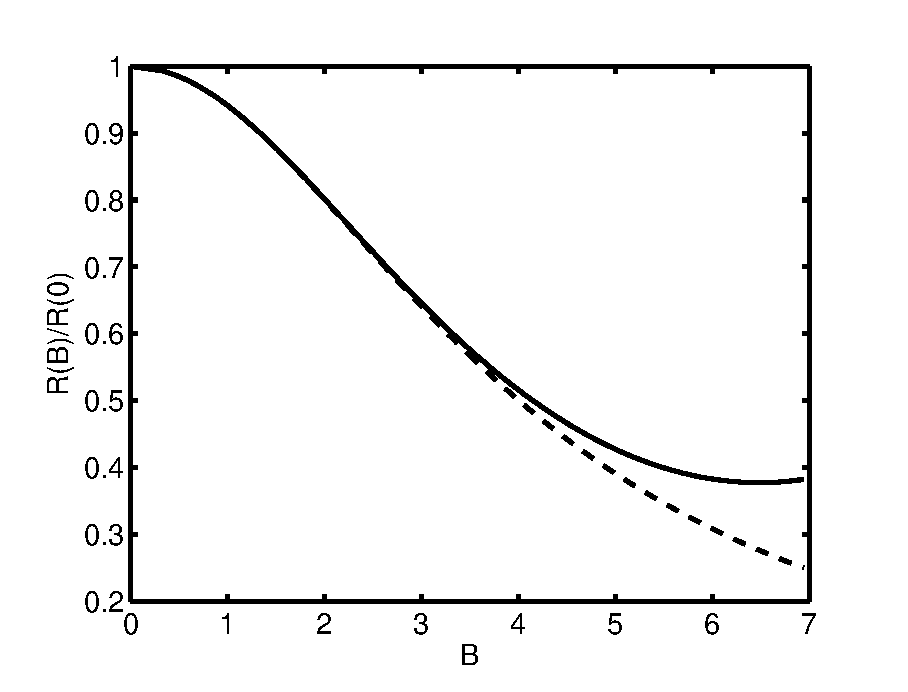
\includegraphics [scale=1] {fig_3_2_1}
	\caption{Зависимость относительного сопротивления от магнитного поля для нанопроволоки висмута ($d=80 \text{ nm}$, $T=4.2\text{ K}$). Пунктирной линией показана зависимость $R(H)/R(0)$ при учете рассеяния носителей на поверхности, сплошной линией при учете рассеяния носителей на шероховатой поверхности и на акустических фононах.} 
	\label{img:fig_3_2_1} 
\end{figure}           % Глава 3
\chapter{Явления переноса в наноструктурах в поперечном электрическом поле с учетом рассеяния на шероховатой поверхности} \label{chapt4}

\section{Исследования подвижности носителей в квантовых ямах в постоянном поперечном электрическом поле} \label{sect4_1}

Расчет электропроводности проведем аналогично тому как это делалось в главе~\ref{chapt3}, используя формулу Кубо \cite{Kubo1957a}. В приближении времени релаксации \cite{Khamidullin2002} конечное выражение для электропроводности может быть записано в следующем виде (слабое тянущее электрическое поле направлено вдоль оси OX)
\begin{equation} \label{eq:41_50}
\sigma _{xx} =\frac{e^{2} }{k_{0} TVm^{2} } \sum _{\alpha ,\beta }\left|P_{\alpha \beta }^{\left(x\right)} \right|^{2} \tau _{\alpha } n_{\alpha } \left(1-n_{\beta } \right) ,
\end{equation} 
$\alpha (\beta )$ -- квантовые числа, описывающие состояние электрона, V -- объем основной области размерно-квантованной системы, $P_{\alpha \beta }^{\left(x\right)} $ -- матричный элемент x-ой компоненты оператора импульса на волновых функциях электрона в зоне проводимости, $n_{\alpha } $ -- равновесная функция распределения носителей с энергией $E_{n,k_{\bot } } $, ${1 \mathord{\left/{\vphantom{1 \tau _{\alpha } }}\right.\kern-\nulldelimiterspace} \tau _{\alpha } } $ --квантово-механическая вероятность рассеяния электронов на шероховатой поверхности:
\begin{equation} \label{eq:41_60}
\frac{1}{\tau _{\alpha } } =\frac{2\pi }{\hbar } \sum _{\beta }\tilde{W}_{\alpha \beta } \delta \left(E_{\alpha } -E_{\beta } \right) V_{\alpha } V_{\beta } ,
\end{equation}
где  
\[
\tilde{W}_{\alpha \beta } =\int \Psi _{\alpha }^{*} \left(r\right)\Psi _{\beta }^{*} \left(r_{1} \right)F^{(\delta )} \left(x-x_{1} ,y-y_{1} \right)\Psi _{\alpha } \left(r_{1} \right)\Psi _{\beta } \left(r\right)drdr_{1}  .
\] 
$\Psi _{i} \left(r\right)$ $i=(\alpha ,\beta )$-- волновые функции электрона в ПКЯ в поперечном электрическом поле \cite{Sinyavskii1998}.

После суммирования по $k_{\bot } $ в \eqref{eq:41_50} электропроводность можно записать в виде:
\begin{equation} \label{eq:41_80}
\sigma _{xx} =\frac{e^2 }{a\pi \hbar^2 \beta_0 } \sum_n\tau_n \ln \left(1+e^{-\beta \xi_n } \right),\;
\xi_n =E_n -\xi ,
\end{equation}
$\xi $ -- химический потенциал исследуемой наноструктуры.

Для невырожденного электронного газа $(\beta _{0} \xi _{n} \gg 1)$ при низких температурах, когда все носители находятся в нижайшей размерно-квантованной зоне проводимости $(n=0)$, подвижность определяется соотношением:
\begin{equation} \label{eq:41_90}
\mu _{xx} =\mu _{xx} (0)\frac{1}{\left(1+2 N_c \right)^2 } , 
\end{equation}
где
\[
\mu _{xx} (0)=\frac{e}{m} \left(\frac{\hbar a^4 }{2\gamma_0 \Delta E_c } \right),
\] 
подвижность в ПКЯ в отсутствии поперечного электрического поля.

Для параметров ПКЯ $(m_e = 0.06 m_0 )$ $\hbar \omega = 14.5/a_0 \text{ eV}$ ($a_0 $ --- ширина ПКЯ в ангстремах), $N_c =1.7\cdot 10^{-18} E_0^2 a_0^3 $ ($E_0 $ -- измеряется в V/cm). Таким образом, при $a_0 = 10^3 \AA$, $E_0 = 2.5\cdot 10^4 \text{ V/cm}$, $N_c =1$, подвижность уменьшается почти на порядок. С ростом $E$ носители тока «прижимаются» к одной из поверхностей квантовой ямы, поэтому их взаимодействие с шероховатой поверхностью увеличивается, что приводит к уменьшению времени релаксации, а следовательно и подвижности.

С ростом температуры процессы рассеяния носителей на длинноволновых акустических колебаниях начинают влиять на величину подвижности. Для случая упругого рассеяния электронов, находящихся на нижайшем уровне зоны проводимости $n=0$ $(\hbar \omega \gg k_B T)$, на акустических фононах при высоких температурах $(N_q \approx \frac{k_BT}{hvq} \gg 1)$ время релаксации определяется соотношением:
\begin{equation} \label{eq:41_100}
\frac{1}{\tau _{f} } =\left(\frac{m\omega }{2\pi \hbar } \right)^{\frac{1}{2} } \frac{E_1^2 m k_B T}{\hbar^3 v^2 \rho } , 
\end{equation} 
$E_1 $~---~константа деформационного потенциала для электрона, $\rho $ -- плотность исследуемой квантовой системы, $v$~--~скорость звука, $N_q $~---~функция распределения равновесных фононов.

Заметим, что $\tau _{f} $ не зависит от волнового вектора электрона и поперечного электрического поля. Электропроводность с учетом рассеяния носителей на шероховатой поверхности $\tau_0 $ и на акустических фононах $\tau_f $ определяется соотношением \eqref{eq:41_80}, в котором согласно правилу Матиссена
\[
\frac{1}{\tau_n } =\frac{1}{\tau_0 } +\frac{1}{\tau_f } .
\]
Конечное выражение для подвижности принимает вид:
\begin{equation} \label{eq:41_110}
\mu _{xx} =\mu _{xx} (0)\frac{1}{\left(1+2N_{c} \right)^{2} +\Delta } , 
\end{equation} 
\[
\Delta =\left(\frac{m\omega }{2\pi \hbar } \right)^{\frac{1}{2} } \left(\frac{E_{1} }{\hbar \omega } \right)^{2} \frac{4k_{B} Ta^{2} }{\rho v^{2} \gamma }. 
\] 

Для ПКЯ с параметрами ($E_{1} =10{\mathrm \; eV}$,$\rho =4{\mathrm \; }{{\mathrm g} \mathord{\left/{\vphantom{{\mathrm g} {\mathrm cm}^{{\mathrm 3}} }}\right.\kern-\nulldelimiterspace} {\mathrm cm}^{{\mathrm 3}} } $,$v=3\cdot 10^{5} {\mathrm \; }{{\mathrm cm} \mathord{\left/{\vphantom{{\mathrm cm} {\mathrm s}}}\right.\kern-\nulldelimiterspace} {\mathrm s}} $,$\gamma ^{{\tfrac{1}{4}} } =40 \AA$) при $E=2.5\cdot 10^{4} {\mathrm \; V/cm}$ рассеяние носителей на акустических колебаниях определяет величину подвижности при $T\ge 100{\mathrm \; K}$.

С ростом напряженности поперечного электрического поля минимум зоны проводимости смещается в запрещенную зону на $\Delta _{c} $, а экстремум валентной зоны поднимается на величину $\Delta _{v} ={e^{2} E^{2}  \mathord{\left/{\vphantom{e^{2} E^{2}  (2m_{v} }}\right.\kern-\nulldelimiterspace} (2m_{v} } \omega _{v}^{2} )$ ($\hbar \omega _{v} $ -- шаг размерного квантования валентной зоны). Следовательно, ширина запрещенной зоны E${}_{g}$ в рассматриваемой модели низкоразмерных систем уменьшается на $\Delta _{c} +\Delta _{v} $. Именно это обстоятельство приводит к тому, что с увеличением E однозонное приближение при исследовании явлений переноса может оказаться не достаточным. В этом случае для расчета электропроводности необходимо учитывать нестандартность зоны проводимости \cite{Lax1960,Cohen1961}. Это приводит к тому, что процессы рассеяния электрона на акустических колебаниях становятся зависящими от E. Отметим, что рассмотренное нами влияние поперечного поля E на электропроводность принципиально отличается от эффекта поля в условиях размерного квантования, исследованного в \cite{Sandomirsky1967,Butenko1998}. В этих работах низкоразмерная система (пленка висмута) являются одной из обкладок конденсатора, и ее заряжают, прикладывая поле E, изменяя в ней концентрацию заряда. Именно поэтому при фиксированной толщине КЯ меняется положение уровня Ферми, что приводит к зависимости электропроводности от величины поперечного электрического поля.

\section{Влияние поперечного электрического поля на подвижность в нанопроволоках} \label{sect4_2}

Для квантовых проволок электрическое поле E, направленное перпендикулярно оси наноструктуры, может заметным образом влиять на кинетические явления в размерно-ограниченной системе. В модели потенциала в форме параболоида вращения (такая модель часто применяется при расчетах кинетических коэффициентов в нанопроволоках \cite{Geiler1998,Cros1992} и находит свое математическое подтверждение \cite{Beenakker1991}), в поперечном электрическом поле E энергия электронов с эффективной массой $m_{c} $ в размерно-квантованной зоне проводимости $c$ и энергетический спектр дырок с эффективной массой $m_{v} $ в валентной зоне $v$ имеют вид:
\begin{equation} \label{eq:42_10}
\begin{aligned}
E_{\alpha }^{c} =\frac{\hbar ^{2} k_{x}^{2} }{2m_{c} } +E_{nm}^{c} \textbf{ ; } E_{nm}^{c} =\hbar \omega _{c} \left(n+k+1\right)-\Delta _{c} ,\\
E_{\alpha }^{v} =\Delta -\frac{\hbar ^{2} k_{x}^{2} }{2m_{v} } +E_{nm}^{v} \textbf{ ; } E_{nm}^{v} =\hbar \omega _{v} \left(n+k+1\right)-\Delta _{v} . (1)
\end{aligned}
\end{equation}


Здесь $\hbar \omega _{c} $ -- шаг размерного квантования в c зоне, $\hbar \omega _{v} $ -- энергия размерного квантования в валентной зоне, которые простым образом связаны с величиной потенциальной энергии $\Delta E_{i} $ на границе нанопроволоки диаметром a,
\[\hbar \omega _{i} =\frac{2\hbar }{a} \sqrt{\frac{2\Delta E_{i} }{m_{i} } } ,\] 
\[\Delta _{c} =\frac{e^{2} E^{2} }{2m_{c} \omega _{c}^{2} } , \Delta _{v} =\frac{e^{2} E^{2} }{2m_{v} \omega _{v}^{2} } ,\] 
$k_{x} $ -- волновой вектор носителя вдоль оси нанопроволоки.

\begin{figure}[h] 
	\center
	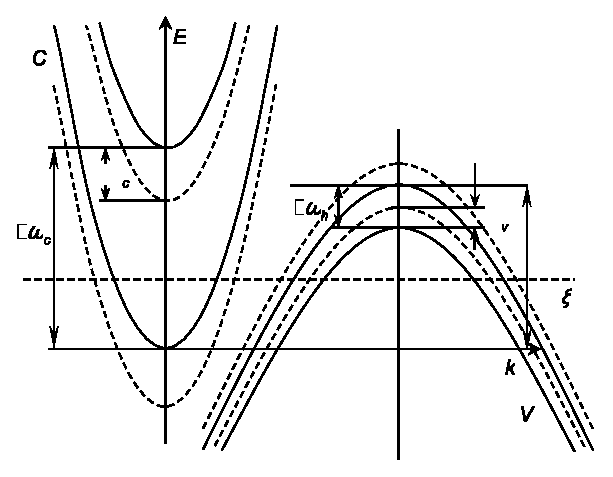
\includegraphics [scale=1] {4_2_1}
	\caption{Схема зонной структуры, рассматриваемой низкоразмерной структуры. Сплошными линиями показаны две нижайшие размерно-квантованные зоны (с-- зоны проводимости, v -- валентные зоны) , пунктирными линиями изображены две нижайшие размерно-квантованные зоны в поперечном электрическом поле; $\xi $ -- химический потенциал.} 
	\label{img:fig_4_2_1} 
\end{figure}

В дальнейшем рассматриваем квантовую проволоку Bi в простой модели, энергетический спектр которой изображен на рис. \ref{img:fig_4_2_1} . Как следует из \eqref{eq:42_10}, с ростом напряженности электрического поля $E$ дно размерно-квантованных c зон опускается на $\Delta _{c} $ в область запрещенных значений энергии, а экстремумы размерно-квантованных v зон поднимаются вверх на величину $\Delta _{v} $.

В квантовых проволоках, как следствие одномерности квантовой системы, на дне размерно-квантованных зон возникают особенности в плотности энергетических состояний. Поэтому, если рассматривать случай вырожденного электронного (дырочного) газа, то с ростом E экстремумы, например размерно-квантованных c зон, опускаясь вниз, пересекают химический потенциал, что может приводить к особенностям электропроводности (подвижности) в исследуемой наноструктуре.

Расчет электропроводности проведем, используя формулу Кубо \cite{Kubo1957a}. В приближении времени релаксации \cite{Khamidullin2002} выражение для электронной электропроводности записывается следующим образом (слабое тянущее электрическое поле направлено вдоль оси нанопроволоки):
\begin{equation} \label{eq:42_20}
\sigma _{xx}^{(e)} =\frac{e^{2} }{k_{0} TVm_{c}^{2} } \sum _{\alpha \beta }\left|\hat{P}_{\alpha \beta }^{(x)} \right|^{2} \tau _{\alpha }^{(e)} n_{\alpha } \left(1-n_{\beta } \right),
\end{equation} 
$\alpha ,\beta $ -- квантовые числа, описывающие состояние электрона, V -- объем основной области размерно-квантованной системы, T -- температура, $k_{0} $ -- постоянная Больцмана, $\hat{P}_{\alpha \beta }^{(x)} $ -- матричный элемент x-ой компоненты оператора импульса на волновых функциях электрона в нанопроволоке, $n_{\alpha } $ -- равновесная функция распределения носителей с энергией $E_{\alpha } $; ${1 \mathord{\left/{\vphantom{1 \tau _{\alpha }^{(e)} }}\right.\kern-\nulldelimiterspace} \tau _{\alpha }^{(e)} } $ -- квантово-механическая вероятность рассеяния в единицу времени.

В дальнейшем исследуем случай рассеяния носителей на шероховатой поверхности, которое оказывается наиболее важным при низких температурах \cite{Sakaki1987,Vurgaftman1999}. В направлении x свободного движения носителей заряда в квантовой проволоке диаметр $a$ меняется случайным образом и, следовательно, энергия размерного квантования $E_{nm}^{(i)} $, зависящая от $a$, флуктуирует. Именно по этой причине энергию взаимодействия носителей с шероховатой поверхностью записывают в виде \cite{Sakaki1987}:
\begin{equation} \label{eq:42_30}
W_{nk}^{(i)} =\frac{\partial E_{nm}^{(i)} }{\partial a} \Delta (x)=-\frac{1}{a} \left[\hbar \omega _{i} \left(n+k+1\right)+2\Delta _{i} \right]\Delta (x)\equiv V_{nk} \Delta (x),  (3)
\end{equation}  
$\Delta (x)$ -- случайная функция.

Как следует из \eqref{eq:42_30}, энергия взаимодействия носителей с шероховатой поверхностью определяется величиной напряженности поперечного электрического поля и с ростом $E$ увеличивается. Последнее обстоятельство приводит, как будет показано ниже, к заметной зависимости подвижности от величины поперечного электрического поля.

Для $\delta $-образной флуктуации поверхности автокорреляционная функция для различных точек поверхности нанопроволоки имеет вид:
\begin{equation} \label{eq:42_40}
\left\{\Delta (x)\Delta (x')\right\}=\gamma \delta (x-x'),
\end{equation} 
Обратим внимание, что вид флуктуации ($\delta $-образный или гауссовый \cite{Sakaki1987}) при низких температурах практически не влияет на конечные результаты физической величины (например на подвижность).

Расчет времени релаксации $\tau _{\alpha } $ проводится аналогично \cite{Karapetyan2011}:
\begin{equation} \label{eq:42_50}
\frac{1}{\tau _{\alpha } } =\frac{2m_c \omega_c^2 \gamma }{\hbar a^2 \left|k_x \right|} \left(n+k+1+N_c \right)^2 , N_c =\frac{2\Delta_c }{\hbar \omega_c } .
\end{equation} 
Согласно \eqref{eq:42_50} время релаксации зависит от всех квантовых чисел, определяющих состояние носителя, и при $N_c = 0$ в точности совпадает с транспортным временем релаксации, используемом при решении кинетического уравнения Больцмана.

Если использовать \eqref{eq:42_20} и \eqref{eq:42_50}, то выражение для подвижности носителей в рассматриваемой модели принимает вид:
\begin{equation} \label{eq:42_60}
\mu =\mu _{0} \frac{\sqrt{\pi } }{2\sum _{nm}F(\eta _{nm}^{c} ) } \sum _{nm}\left\{\frac{\ln \left[\exp \left(\eta _{nm}^{c} \right)+1\right]}{\left(n+m+1+N_{c} \right)^{2} } +\left(\frac{\Delta E_{c} }{\Delta E_{v} } \right)\frac{1}{p} \frac{\ln \left[\exp \left(\eta_{nm}^v \right)+1\right]}{\left(n+m+1+N_v \right)^2 } \right\} . 
\end{equation} 
Здесь введены обозначения:
\[
\eta_{nm}^c =\frac{1}{k_0 T} \left[\xi -\hbar \omega_c \left(n+m+1\right)+\Delta_c \right],
\] 
\[
\eta_{nm}^v =\frac{1}{k_0 T} \left[-\xi -\hbar \omega_v \left(n+m+1\right)+\Delta_0 +\Delta_v \right],
\] 
\[
\mu_0 =\frac{4R^4 e}{\gamma \Delta E_c } \sqrt{\frac{k_0 T}{2\pi m_c } }, \;
R=\frac{a}{2}, \;
N_c =\frac{2\Delta_c }{\hbar \omega_c }, \;
N_v =\frac{2\Delta_v }{\hbar \omega_v },
\] 
\[
F(\eta_{nm}^c )=\int_0^{\infty }{\frac{dx}{\exp \left(x^2 -\eta_{nm}^c \right)+1}}  ,
\] 
$p$ --- число $c$ зон, участвующих в процессах электропроводности. Химический потенциал $\xi $ находится из условия электронейтральности исследуемой наноструктуры (число электронов в зонах проводимости равно числу дырок в валентной зоне)
\begin{equation} \label{eq:42_70}
p\sqrt{\frac{m_{c} }{m_{v} } } \sum _{n,m}\int _{0}^{\infty }\frac{dx}{\exp \left(x^{2} -\eta _{nm}^{c} \right)+1}   =\sum _{n,m}\int _{0}^{\infty }\frac{dx}{\exp \left(x^{2} -\eta _{nm}^{v} \right)+1}. 
\end{equation} 
Положение химического потенциала при заданных параметрах наносистемы определяется величиной радиуса R квантовой проволоки и величиной напряженности поперечного электрического поля.

Рассмотрим частные случаи, допускающие аналитическое решение уравнения \eqref{eq:42_70}. Пусть электронный (дырочный) газ является невырожденным. Это возможно, если радиус квантовой проволоки такой, что $\Delta_0 < \hbar \omega_c +\hbar \omega_v $. Как показали экспериментальные исследования \cite{Black2003a} при $R=250 \AA$ в нанопроволоках Bi $\Delta_0 =\hbar \omega_c +\hbar \omega_v $. Если $m_c \ll m_{v} $ и носители находятся в нижайших размерно-квантованных зонах $(n = m = 0)$, подвижность можно записать в следующем виде:
\begin{equation} \label{eq:42_80}
\mu =\mu _{0} \frac{1}{\left(1+N_{c} \right)^{2} } .
\end{equation}

\begin{figure}[!h] 
	\center
	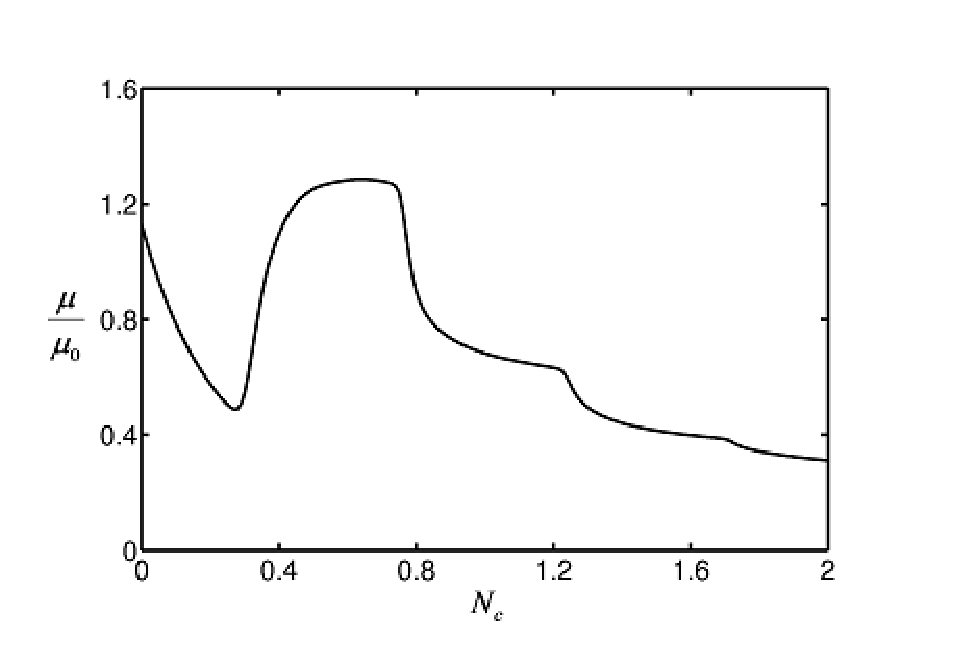
\includegraphics [scale=1] {image402}
	\caption{Зависимость подвижности (в относительных единицах) от напряженности поперечного электрического поля. $R=330 \AA$.} 
	\label{img:fig_4_2_2} 
\end{figure}

\begin{figure}[!h] 
	\center
	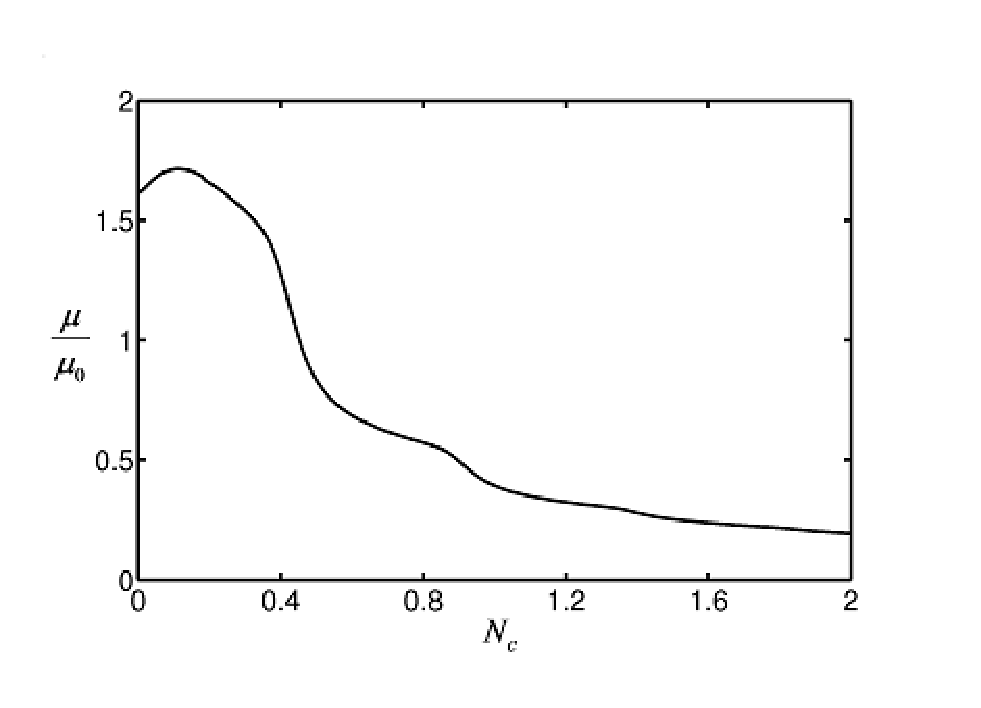
\includegraphics [scale=1] {image403}
	\caption{Зависимость подвижности (в относительных единицах) от напряженности поперечного электрического поля. $R=990 \AA$.} 
	\label{img:fig_4_2_3} 
\end{figure}

Согласно \eqref{eq:42_80} подвижность в рассматриваемом случае с ростом напряженности поперечного электрического поля убывает. Это связано с более сильным взаимодействием носителей с шероховатой поверхностью с увеличением электрического поля. Если электронный газ вырожден и химический потенциал расположен между нижайшей и последующей размерно-квантованной зоной проводимости (аналогично и для размерно-квантованной v зоны), то подвижность описывается следующим соотношением:
\begin{equation} \label{eq:42_90}
\mu =\mu_0 \frac{\sqrt{2\pi}}{4\left(1+N_c \right)^2 } \left[\frac{1}{k_0 T} \left(\Delta_0 +\Delta_c +\Delta_v -\hbar \omega_v -\hbar \omega_c \right)\right]^{\frac{1}{2} }
\end{equation} 

Как непосредственно следует из \eqref{eq:42_90}, подвижность с ростом E убывает, но слабее, чем в случае невырожденного электронного газа. В общем случае зависимость подвижности от напряженности поперечного электрического поля можно найти только численно.

Влияние поперечного электрического поля на подвижность принципиальным образом зависит от радиуса нанопроволоки. При небольших значениях $R$, когда квантовая проволока представляет почти безщелевой полупроводник, с ростом $E$ (при $E=0$ электронный (дырочный) газ невырожден) подвижность сначала уменьшается (см формулу \eqref{eq:42_80}), затем увеличивается, и в дальнейшем описывается осцилляционной кривой (рисунок~\ref{img:fig_4_2_2}). При больших радиусах нанопроволок, когда электронный (дырочный) газ изначально был вырожден, зависимость $\mu$ от $E$ носит явно осциллирующий характер (рисунок~\ref{img:fig_4_2_3}). Такое поведение подвижности в присуствии поперечного электрического поля связано с тем, что с ростом напряженности поперечного электрического поля, дно размерно-квантованных $c$ зоны, опускаясь в область запрещенных значений энергии, пересекает химический потенциал, что приводит к увеличению подвижности. Заметим, что для типичных значений параметров нанопроволок Bi ($m_c = 0.01m_0 $, $m_v = 0.1m_0$, $\Delta E_c  / \Delta E_v  = 1.5$) $N_v =5.8 N_c $, поэтому с ростом $E$ влияние дырок на поведение $\mu$ от $E$ слабее, чем для электронов. Следовательно, осцилляционная зависимость подвижности от $E$ (рисунок~\ref{img:fig_4_2_3}) должна наблюдаться и для полупроводниковых квантовых проволок с вырожденным электронным газом.

\section{Особенности подвижности в нанопроволоках в поперечных электрическом и магнитном полях} \label{sect4_3}
Теперь рассмотрим одновременное влияние магнитного и электрического полей на явления переноса в квантовых проволоках. В присутствии однородного квантующего магнитного поля энергетический спектр носителей в квантовых проволоках заметным образом меняется. В модели параболического потенциала для нанопроволок радиуса $R$ энергия электрона с учетом анизотропии эффективных масс (магнитное поле H  направлено перпендикулярно оси наноструктуры, электрическое поле E параллельно H) определяется аналогично \cite{Geiler1998}.

\begin{equation} \label{eq:43_10}
	E_{k_x,n,m}=\frac{{\hbar }^2k^2_x}{2m^*_x}+\hbar {\Omega }_y\left(n+\frac{1}{2}\right)+\hbar {\omega }_z\left(m+\frac{1}{2}\right)-{\Delta }_c,   
\end{equation}
\[
m^*_x=m_x{\left(\frac{{\Omega }_y}{{\omega }_y}\right)}^2,\ \ {\Omega }^2_y=\frac{m_x}{m_y}{\left({\omega }^c_x\right)}^2+{\omega }^2_y,\ \ {\omega }^c_x=\frac{eH}{m_xc},\ \ {\omega }_i=\frac{1}{R}{\left[\frac{2\Delta E_c}{m_i}\right]}^{\frac{1}{2}},\ \ {\Delta }_c=\frac{{\left(eER\right)}^2}{4\Delta E_c}
\]
$k_x$ -- волновой вектор электрона вдоль оси квантовой проволоки, $\hbar {\omega }_z,\ \ \hbar {\Omega }_y$ -- энергии размерного квантования, $\Delta E_c$ -- высота потенциальной энергии на границе наноструктуры.

Заметим, что с ростом напряженности электрического поля дно размерно-квантованной зоны проводимости опускается в область запрещенной зоны.

Расчет тензора электропроводности проведем с использованием формулы Кубо
\cite{Kubo1957a} (слабое тянущее электрическое поле направлено вдоль оси нанопроволоки). В приближении времени релаксации \cite{Khamidullin2002} электропроводность записывается следующим образом 

В дальнейшем рассмотрим случай рассеяния заряженных частиц на шероховатой поверхности наносистемы \cite{Sakaki1987},  который является доминирующим при малых радиусах квантовой проволоки и низких температурах. При этом энергию взаимодействия носителей с шероховатой поверхностью записываем в следующем виде \cite{Sakaki1987,Motohisa1992}:
\begin{equation} \label{eq:43_30} 
W_{\alpha }=\frac{\partial E_{\alpha }}{\partial R}\Delta \left(x\right)\equiv V_{\alpha }\Delta \left(x\right) 
\end{equation}
\[
V_{\alpha }=-\frac{1}{R}\left[{\left(\frac{{\omega }_y{\omega }^c_x}{{\Omega }^2_y}\right)}^2\frac{m_y}{m_x}\frac{{\hbar }^2k^2_x}{m_x}+\hbar {\omega }_y\left(\frac{{\omega }_y}{{\Omega }_y}\right)\left(n+\frac{1}{2}\right)+\hbar {\omega }_z\left(m+\frac{1}{2}\right)+2{\Delta }_c\right]
\] 
$\Delta \left(x\right)$ -- случайная функция.

Для $\delta $-образной флуктуации поверхности автокорреляционная функция для различных точек поверхности имеет вид:
\[
\left\{\Delta \left(x\right)\Delta \left(x'\right)\right\}={\gamma }_0\delta \left(x-x'\right),
\] 
а усреднение проводится по реализации случайного процесса.  Как непосредственно следует из \eqref{eq:43_30}, с ростом напряженности поперечного электрического поля E взаимодействие электрона с шероховатой поверхностью увеличивается. Расчет времени релаксации с учетом \eqref{eq:43_30} проводится аналогично \cite{Karapetyan2011}. В результате
\begin{equation} \label{eq:43_40} 
\frac{1}{{\tau }_{\alpha }}={\Gamma }_{\alpha }\frac{1}{\left|k_x\right|},\ {\Gamma }_{\alpha }=\frac{2{\gamma }_0m^*_x}{{\hbar }^3}V^2_{\alpha }.  
\end{equation}
Заметим, что время релаксации \eqref{eq:43_40} в точности равно транспортному времени релаксации, используемому при решении кинетического уравнения Больцмана.

Если учесть, что матричный элемент импульса определяется соотношением\footnote{Недиагональные по осцилляторному квантовом числу матричные элементы при разумных параметрах КП дают незначительный в искомую электропроводность}:
\[
{\hat{P}}^{\left(x\right)}_{\alpha \beta }=\hbar k_x{\left(\frac{{\omega }_y}{{\Omega }_y}\right)}^2{\delta }_{\alpha \beta },
\] 
то выражение для электропроводности \eqref{eq:43_20} с учетом \eqref{eq:43_40} принимает вид \eqref{eq:42_20};

В дальнейшем рассматриваем низкие температуры, когда $\hbar {\omega }_z\gg k_0T$, поэтому зависимостью $V_{\alpha }$ от волнового вектора электрона можно пренебречь. В этом естественном приближении соотношение \eqref{eq:43_50}, после интегрирования по $k_x$, можно записать:
\begin{equation} \label{eq:43_60}
{\sigma }_{xx}=\frac{2e^2\hbar }{{\beta }_0{\pi }^2m^*_x{\gamma }_0}\sum_{nm}{\frac{{ln \left[1+{exp \left({\beta }_0{\xi }_{nm}\right)\ }\right]\ }}{{\left[\hbar {\omega }_y\frac{{\omega }_y}{{\Omega }_y}\left(n+\frac{1}{2}\right)+\hbar {\omega }_z\left(m+\frac{1}{2}\right)+2{\Delta }_c\right]}^2}} 
\end{equation}
\[
{\xi }_{nm}=\xi -\hbar {\Omega }_y\left(n+\frac{1}{2}\right)-\hbar {\omega }_z\left(m+\frac{1}{2}\right)+{\Delta }_c,\ \ \beta =\frac{1}{k_0T}
\]
$\xi $ -- химический потенциал исследуемой наносистемы. Аналогично можно записать ${\sigma }_{xx}$ для дырок в T валентной зоне полуметалла Bi. В этом случае в \eqref{eq:43_60} эффективные массы электронов нужно заменить на соответствующие массы дырок ${\mu }_x,{\mu }_y,{\mu }_z$, а $\xi $  на $-\xi +{\Delta }_0$ (${\Delta }_0$ определяется перекрыванием T валентной зоны и зоны проводимости, ${\Delta }_0\cong 39\ meV$ \cite{Levin2009a}) 

Энергия электронов в валентной зоне определяется соотношением:
\[
E^v_{\alpha }={\Delta }_0-\frac{{\hbar }^2k^2_x}{2{\mu }^*_x}-\hbar {\widetilde{\Omega }}_y\left(n+\frac{1}{2}\right)-\hbar {\widetilde{\omega }}_z\left(m+\frac{1}{2}\right)+{\Delta }_v,
\] 
здесь обозначено
\[
{\mu }^*_x={\mu }_x{\left(\frac{{\widetilde{\Omega }}_y}{{\widetilde{\omega }}_y}\right)}^2,\ {\widetilde{\Omega }}^2_y=\frac{{\mu }_x}{{\mu }_y}{\left({\widetilde{\omega }}^c_x\right)}^2+{\widetilde{\omega }}^2_y,\ \ {\widetilde{\omega }}^c_x=\frac{eH}{{\mu }_xc},\ \ {\widetilde{\omega }}_i=\frac{1}{R}{\left[\frac{2\Delta E_v}{{\mu }_i}\right]}^{\frac{1}{2}},\ \ {\Delta }_v=\frac{{\left(eER\right)}^2}{4\Delta E_v}
\] 
$\hbar {\widetilde{\Omega }}_y, \hbar {\widetilde{\omega }}_z$ -- энергия размерного квантования в валентной зоне, $\Delta E_v$ -- высота потенциальной энергии для дырок на границе квантовой проволоки.

Следовательно, подвижность носителей (электронов и дырок) в нанопроволоке записывается следующим образом:
\begin{multline} \label{eq:43_70} 
\mu =\frac{eR^2{\hbar }^2}{m^*_x{\gamma }_0}\frac{1}{\sqrt{2m^*_x{\beta }_0}\sum_{nm}{F\left({\xi }_{nm}\right)}}\sum_{nm}{\frac{{\ln \left[1+{\exp \left(\beta {\xi }_{nm}\right)\ }\right]\ }}{{\left[\hbar {\omega }_y\frac{{\omega }_y}{{\Omega }_y}\left(n+\frac{1}{2}\right)+\hbar {\omega }_z\left(m+\frac{1}{2}\right)+2{\Delta }_c\right]}^2}}+\\
+\frac{eR^2{\hbar }^2}{{\mu }^*_x{\gamma }_0}\frac{1}{\sqrt{2{\mu }^*_x{\beta }_0}\sum_{nm}{F\left({\widetilde{\xi }}_{nm}\right)}}\sum_{nm}{\frac{{\ln \left[1+{\exp \left(\beta {\widetilde{\xi }}_{nm}\right)\ }\right]\ }}{p{\left[\hbar {\widetilde{\omega }}_y\frac{{\widetilde{\omega }}_y}{{\widetilde{\Omega }}_y}\left(n+\frac{1}{2}\right)+\hbar {\widetilde{\omega }}_z\left(m+\frac{1}{2}\right)+2{\Delta }_v\right]}^2}} 
\end{multline}
\[
F\left({\xi }_{nm}\right)=\int^{\infty }_0{\frac{dx}{{exp \left(x^2-\beta {\xi }_{nm}\right)\ }+1}},
\]
\[
{\widetilde{\xi }}_{nm}=-\xi -\hbar {\widetilde{\Omega }}_y\left(n+\frac{1}{2}\right)-\hbar {\widetilde{\omega }}_z\left(m+\frac{1}{2}\right)+{\Delta }_0+{\Delta }_v
\]
p -- число С зон, участвующих в процессах электропроводности. Если магнитное поле направлено вдоль оси OZ, а постоянное поперечное электрическое поле E перпендикулярно H, то подвижность, как показывают расчеты, тоже описывается соотношением \eqref{eq:43_70}.

Химический потенциал $\xi $ находится из условия электронейтральности исследуемой квантовой проволоки (число электронов в p зонах проводимости равно числу дырок в валентной зоне):
\begin{equation} \label{eq:43_80} 
p{\left(\frac{m^*_x}{{\mu }^*_x}\right)}^{\frac{1}{2}}\sum_{nm}{F\left({\xi }_{nm}\right)}=\sum_{nm}{F\left({\widetilde{\xi }}_{nm}\right)} (8) 
\end{equation}

Из \eqref{eq:43_80} следует что, величина химического потенциала $\xi $ зависит от радиуса нанопроволоки и определяется напряженностью электрического и магнитного полей.

Дальнейшие оценки будем проводить для параметров, близких к полуметалу Bi: $m_x=0.0011m_0$, $m_y=0.26m_0$, $m_z=0.0045m_0$, ${\mu }_x={\mu }_y=0.059m_0$, ${\mu }_z=0.634$ \cite{Levin2009a}, ${\Delta }_c=0.5\ eV$, ${\Delta }_v=0.3\ eV$ ($m_0$ -- масса свободного электрона). При этих параметрах
\[
\hbar {\omega }_y=\frac{4.9}{R_0}\left(eV\right),\ \hbar {\omega }_z=\frac{37.6}{R_0}\left(eV\right),\ \hbar {\widetilde{\omega }}_y=\frac{8}{R_0}\left(eV\right),\ \ \hbar {\widetilde{\omega }}_z=\frac{2.4}{R_0}\left(eV\right)\ ,
\] 
($R_0$ -- радиус нанопроволоки в ангстремах).

\noindent \includegraphics*[width=5.21in, height=4.89in, keepaspectratio=false]{image404}

\noindent Рис. 1. Зависимость подвижности в относительны единицах $\widetilde{{\mathbf \mu }}={{\mathbf \mu }\left(E\right)}/{{\mathbf \mu }\left(0\right)}$ от электрического поля.

На рис. 1 приведены численные расчеты зависимости подвижности (в относительных единицах) от напряженности поперечного электрического поля. Кривые 1,2,3 получены при $\ \delta =0,$ $\delta =0.05$, $\delta =0.1$ соответсвенно $\left(\delta ={\left(\frac{{\omega }^c_x}{{\omega }_y}\right)}^2\right)$. При малых значениях ${\Delta }_c$ электронный газ (при рассмотренных параметрах квантовой проволоки) является невырожденным, поэтому с ростом напряженности поперечного электрического поля уменьшается \cite{Karapetyan2012}. Кривая 1 (подвижность в отсутствии  магнитного поля) описывается тремя максимумами. Такая осцилляционная зависимость подвижности связана с тем, что с ростом $E$ химический потенциал, отсчитанный от дна размерно-квантованной зоны проводимости, поднимается в область больших значений энергии и может «наткнуться» на дно размерно-квантованной C зоны, в которой существуют особенности в плотности энергетических состояний. Первый пик связан с пересечением химического потенциала нижайшего состояния размерно-квантованной C зоны $\left(n=0,m=0\right)$, второй пик возникает из-за пересечения химического потенциала дна первой размерно-квантованной зоны $\left(m=0,n=1\right),$ третий пик -- из-за пересечения химического потенциала второй размерно-квантованной зоной $\left(m=1,n=0\right)$. С ростом напряженности магнитного поля дно размерно-квантованной зоны проводимости поднимается в область больших значений энергии, поэтому пересечение химического потенциала наступает при больших значениях ${\Delta }_c$. Именно по этой причине первый пик кривой 2  сдвинут по отношению первого пика кривой 1 в область больших значений напряженности поперечного электрического поля.

Заметим, что согласно \eqref{eq:43_70} подвижность с ростом напряженности магнитного поля уменьшается. Это связано с тем, что эффективные массы электронов (дырок) в однородном поперечном магнитном поле увеличиваются (в ${\left(\frac{\Omega_y}{\omega_y}\right)}^2$ раз для электронов и в ${\left(\frac{{\widetilde{\Omega }}_y}{{\widetilde{\omega }}_y}\right)}^2$ раз для дырок).

\section{Термоэдс в нанопроволоках Bi в попереченом постоянном электрическом поле}\label{sect4_4}

В квантовых проволоках, как следствие одномерности исследуемой наносистемы, на дне размерно-квантованных зон возникают особенности в плотности энергетических состояний. Именно это обстоятельство приводит, в частности, к особенностям оптических свойств нанопроволок \cite{Black2003a,Black2000,Black2002,Levin2009a}, и заметным образом влияет, как будет показано ниже, на кинетические коэффициенты в нанопроволоках с вырожденным электронным (дырочным) газом. В настоящей диссертационной работе теоретически исследуется термоэдс в квантовых проволоках типа Bi в модели квадратичного потенциала. Такая модель часто применяется при расчетах кинетических коэффициентов в нанопроволоках \cite{Geiler1998,Geiler1999} и находит свое теоретическое обоснование \cite{Beenakker1991}. Если постоянное электрическое поле $E$, направленное вдоль оси размерного квантования наноструктуры при определенных условиях может существенным образом влиять на подвижность \cite{Karapetyan2011}, то представляет интерес исследовать влияние $E$ на термоэдс в низкоразмерных системах.
 
В квантовых проволоках типа Bi с потенциальной энергией для носителей в форме параболоида вращения в постоянном электрическом поле E, направленном перпендикулярно оси исследуемой наноструктуры. В рассматриваемой модели энергия электронов с эффективной массой $m_{c} $ в размерно-квантованной зоне проводимости имеет вид:
\begin{equation} \label{eq:44_10}
\varepsilon _{c} =\frac{\hbar ^{2} k_{x}^{2} }{2m_{c} } +\hbar \omega _{c} \left(n+k+1\right)-\Delta _{c} , \Delta _{c} =\frac{e^{2} E^{2} }{2m_{c} \omega _{c}^{2} } , 
\end{equation} 
здесь $k_{x} $ -- волновой вектор носителя вдоль оси нанопроволоки, $\hbar \omega _{c} $ -- шаг размерного квантования, который простым образом связан с величиной потенциальной энергии $\Delta E_{c} $ на границе наноструктуры с радиусом R:
\[
\hbar \omega _{c} =\frac{\hbar }{R} \sqrt{\frac{2\Delta E_{c} }{m_{c} } } .
\] 

Как непосредственно следует из (1) с ростом напряженности электрического поля дно размерно-квантованной зоны проводимости опускается в запрещенную зону. Именно это обстоятельство приводит к тому, что при учете рассеяния электронов на шероховатой поверхности время релаксации зависит от E, что и приводит к заметному изменению кинетических коэффициентов \cite{Karapetyan2011}. С ростом E носители «прижимаются» к поверхности наноструктуры, т.е. их взаимодействие с шероховатой поверхностью увеличивается, что приводит к уменьшению времени релаксации. Аналогичным образом можно вычислить энергию электронов с эффективной массой $m_{v} $ в размерно-квантованной валентной зоне.
\begin{equation} \label{eq:44_20}
\varepsilon _{v} =\Delta -\frac{\hbar ^{2} k_{x}^{2} }{2m_{v} } -\hbar \omega _{v} \left(n+k+1\right)+\Delta _{v} , (2)
\end{equation} 
\[
\Delta _{v} =\frac{e^{2} E^{2} }{2m_{v} \omega _{v}^{2} } , \hbar \omega _{v} =\frac{\hbar }{R} \sqrt{\frac{2\Delta E_{v} }{m_{v} } } 
\] 


\begin{figure}[h] 
	\center
	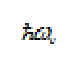
\includegraphics [scale=1] {image408}
	\captionsetup{labelformat=empty}
	\caption{Рис. 1 Схема энергетических зон квантовой проволоки Bi в постоянном электрическом поле} 
	\label{img:fig_4_4_1} 
\end{figure}

  
В дальнейшем для нанопроволок Bi рассмотрим простейшую модель перекрывающихся зон (рис. 1). На рис. 1. сплошными линиями изображены  размерно-квантованные уровни c и v зон. Пунктирными линиями представлены энергии носителей в постоянном электрическом поле.

Расчет термоэдс $\alpha _{xx} $ (слабое тянущее электрическое поле направленно вдоль оси x) проводился с использованием общих соотношений, связывающих $\alpha _{xx} $ с плотностью потока тепловой энергии $\gamma _{xx} $ для носителей и с электропроводностью для электронов и дырок \cite{Kubo1957}. В приближении времени релаксации \cite{Khamidullin2002} электропроводность и плотность потока тепловой энергии для электронов принимают вид:
\begin{equation} \label{eq:44_30}
\sigma _{xx}^{(c)} =\frac{\beta e^{2} \hbar ^{2} }{2Vm_{c}^{2} } \sum _{\alpha }k_{x}^{2} \tau _{\alpha }^{(c)} n_{\alpha } \left(1-n_{\alpha } \right) , (3a)
\end{equation}
\begin{equation} \label{eq:44_31}
\gamma _{xx}^{(c)} =\frac{\beta e^{2} \hbar ^{2} }{2Vm_{c}^{2} } \sum _{\alpha }\left(E_{\alpha }^{c} -\xi \right)k_{x}^{2} \tau _{\alpha }^{(c)} n_{\alpha } \left(1-n_{\alpha } \right) , (3b)
\end{equation}
\noindent здесь $n_{\alpha } $ -- равновесная функция распределения носителей с энергией $E_{\alpha }^{c} $, $\alpha $ -- набор квантовых чисел, описывающих состояние электрона, ${1 \mathord{\left/{\vphantom{1 \tau _{\alpha }^{(e)} }}\right.\kern-\nulldelimiterspace} \tau _{\alpha }^{(e)} } $ -- определяет полную квантово-механическую вероятность рассеяния частицы в единицу времени, $\xi $ -- химический потенциал исследуемой системы, $\beta ={1 \mathord{\left/{\vphantom{1 k_{0} T}}\right.\kern-\nulldelimiterspace} k_{0} T} $, T -- температура, V -- объем основной области наноструктуры.
 
Аналогично можно записать $\sigma _{xx}^{(h)} $, $\gamma _{xx}^{(h)} $ для дырок в v зоне. Расчет времени релаксации $\tau _{\alpha } $ проведем с учетом рассеяния носителей на шероховатой поверхности аналогично \cite{Karapetyan2011}. В случае $\delta $-образной флуктуации поверхности нетрудно получить:
\begin{equation} \label{eq:44_40}
\frac{1}{\tau _{\alpha }^{(c)} } =\frac{2m_{c} \omega _{c}^{2} \gamma _{0} }{\hbar R^{2} \left|k_{x} \right|} \left[n+k+1+N_{c} \right]^{2} , N_{c} =\frac{2\Delta _{c} }{\hbar \omega _{c} } ,
\end{equation} 
$\gamma _{0} $ -- описывает высоту флуктуации. При расчете времени релаксации для случая гауссовой флуктуации \cite{Vurgaftman1999} при низких температурах (именно при низких температурах рассеяние носителей на шероховатой поверхности наиболее активно) ${1 \mathord{\left/{\vphantom{1 \tau _{\alpha }^{(e)} }}\right.\kern-\nulldelimiterspace} \tau _{\alpha }^{(e)} } $ описывается соотношением (4), в котором нужно $\gamma _{0} $ заменить на $\pi \Delta _{0}^{2} \Lambda ^{2} $ ($\Delta _{0} $ -- высота гауссовой флуктуации, $\Lambda $ -- ее длина). Аналогично записывается $\tau _{\alpha }^{(h)} $ для дырок. В результате выражение для термоэдс после суммирования по $k_{x} $ принимает вид:
 
\begin{multline} \label{eq:44_50}
\alpha _{xx} =-\frac{k_{0} }{e} \left\{\sum _{n,m}\left[\nu \frac{F_{2} \left(\eta _{nm}^{c} \right)-\eta _{nm}^{c} F_{1} \left(\eta _{nm}^{c} \right)}{\left(n+m+1+N_{c} \right)^{2} } -\frac{F_{2} \left(\eta _{nm}^{v} \right)-\eta _{nm}^{v} F_{1} \left(\eta _{nm}^{v} \right)}{b\left(n+m+1+aN_{c} \right)^{2} } \right] \right\}\times\\
\times \left\{\sum _{n,m}\left[\nu \frac{F_{1} \left(\eta _{nm}^{c} \right)}{\left(n+m+1+N_{c} \right)^{2} } +\frac{F_{1} \left(\eta _{nm}^{v} \right)}{b\left(n+m+1+aN_{c} \right)^{2} } \right] \right\}^{-1}
\end{multline}
\[
a=\left(\frac{m_{h} }{m_{c} } \right)^{\frac{1}{2} } \left(\frac{\Delta E_{c} }{\Delta E_{h} } \right)^{\frac{3}{2} } , b=\frac{\Delta E_{h} }{\Delta E_{c} } ,
\] 
\[
\eta _{nm}^{c} =\beta \left[\Delta _{c} +\xi -\hbar \omega _{c} \left(n+m+1\right)\right],
\] 
\[
\eta _{nm}^{v} =\beta \left[\Delta +\Delta _{v} -\xi -\hbar \omega _{v} \left(n+m+1\right)\right],
\] 
\[
F_{k} (\eta )=\int _{0}^{\infty }dx \cdot x^{k} \cdot \frac{e^{x-\eta } }{\left(e^{x-\eta } +1\right)^{2} } , F_{1} (\eta )=\ln \left(e^{\eta } +1\right)
\] 
v -- количество зон проводимости, участвующих в кинетических процессах. Химический потенциал $\xi $ определяется из условия электронейтральности исследуемой наноструктуры (число электронов в размерно-квантованных c зонах равно числу дырок в v зоне):
\begin{equation} \label{eq:44_60}
\nu \sqrt{\frac{m_{c} }{m_{v} } } \sum _{n,m}F_{{\raise0.7ex\hbox{$ 1 $}\!\mathord{\left/{\vphantom{1 2}}\right.\kern-\nulldelimiterspace}\!\lower0.7ex\hbox{$ 2 $}} } \left(\eta _{nm}^{c} \right) =\sum _{n,m}F_{{\raise0.7ex\hbox{$ 1 $}\!\mathord{\left/{\vphantom{1 2}}\right.\kern-\nulldelimiterspace}\!\lower0.7ex\hbox{$ 2 $}} } \left(\eta _{nm}^{v} \right) .
\end{equation}
 
Аналитическое решение уравнения \eqref{eq:44_60} для химического потенциала можно найти для частных случаев.
 
Если носители находятся на нижайшем размерно-квантованном уровне ($n=m=0$), электронный и дырочный газ вырожден (химический потенциал положителен и $\beta \xi >>1$), то при $m_{c} <<m_{v} $, из \eqref{eq:44_60} не трудно определить $\xi $:
\[
\xi -\hbar \omega _{c} =\Delta +\Delta _{v} -\left(\hbar \omega _{c} +\hbar \omega _{v} \right), \left(\frac{\Delta _{v} }{\Delta _{c} } =\frac{\Delta E_{c} }{\Delta E_{v} } >1\right).
\] 
$\xi -\hbar \omega _{c} $ -- химический потенциал отсчитываемый от дна размерно-квантованной зоны.

В такой простой модели, термоэдс принимает вид:
\begin{equation} \label{eq:44_70}
\alpha _{xx} =-\frac{k_{0} }{e} \frac{\pi ^{3} }{3} \frac{1-\frac{1}{b\nu } \left(\frac{1+N_{c} }{1+aN_{c} } \right)^{2} }{\Delta +\Delta _{v} -\left(\hbar \omega _{c} +\hbar \omega _{v} \right)} .
\end{equation} 
Следовательно, термоэдс отрицательна, т.е. определяется электронами и с ростом напряженности электрического поля E уменьшается.

В противоположном случае невырожденного электронного и дырочного газов (это справедливо при малых радиусах квантовой проволоки $d<<500 \AA$Е, при $T=77 \text{ K}$ \cite{Black2002}), как следует из уравнения \eqref{eq:44_60}, химический потенциал определяется из соотношения:
\begin{equation} \label{eq:44_80}
\nu \sqrt{\frac{m_{c} }{m_{v} } } \exp \left(\eta _{00}^{c} \right)=\exp \left(\eta _{00}^{v} \right).
\end{equation}  
В результате
\begin{equation} \label{eq:44_90}
\alpha _{xx}^{(nd)} =-\frac{k_{0} }{e} \left\{2+\beta \left[\frac{1}{2} \ln (\nu ^{2} \frac{m_{c} }{m_{h} } )+\left(\hbar \omega _{c} +\hbar \omega _{v} -\Delta +\Delta _{v} +\Delta _{c} \right)\right]\right\},
\end{equation} 
 
Расчет термоэдс в общем случае проведен по соотношению \eqref{eq:44_50} с учетом размерно-квантованных v и c зон при типичных значениях параметров квантовой проволоки: $\Delta E_{c} =0.5 \text{ eV}$, $\Delta E_{v} =0.3 \text{ eV}$, $\Delta =0.038 \text{ eV}$, $m_{c} =0.01m_{0} $, $m_{v} =0.1m_{0} $, при $R=500 \AA$. Зависимость термоэдс от напряженности постоянного электрического поля приведена на рис. 2. 
 
\noindent \includegraphics*[width=6.16in, height=3.75in, keepaspectratio=false]{image414}
 
\noindent Рис. 2, Зависимость удельной термоэдс квантовой проволоки от напряженности поперечного электрического поля.
 
Кривая 1 получена при $T=10 \text{ K}$, кривая 2 вычислена при $T=50 \text{ K}$. Как показано на рис. 2. с ростом температуры величина термоэдс по абсолютной величине уменьшается и при увеличении E, стремится к нулю оставаясь при этом отрицательной.
 
В нанопроволоках, как следствие одномерности наноструктуры в плотности состояний на дне каждой размерно-квантованной зоны возникают особенности. Поэтому с ростом напряженности постоянного электрического поля экстремумы, например, размерно-квантованных v зон, поднимаясь вверх по энергии, могут пересекать химический потенциал, что, естественно, приводит к особенностям кинетических коэффициентов (например, подвижности). Однако в термоэдс эти особенности не очень ярко проявляются, поскольку $\alpha _{xx} $ определяется отношением потока тепловой энергии носителей к электропроводности.
 
При $E=0$ дырки вносят заметный вклад в термоэдс, уменьшая ее по абсолютной величине. С ростом напряженности электрического поля (для рассмотренных выше параметров нанопроволоки $a\sim 7$) вклад дырок в термоэдс быстро уменьшается, а это и приводит к тому, что в зависимости $\alpha _{xx} $ от $N_{c} $ (рис. 2) возникает характерный минимум.
 
Следовательно, внешнее электрическое поле дает уникальную возможность управлять величиной термоэдс, что позволяет надеяться  на приборное применение предсказанного эффекта. В заключение отметим, что сильная анизотропия эффективных эффективных масс в нанопроволоках Bi(в зависимости от направления кристаллографических осей массы для электронов в С-зоне меняются от $0,001m_{0} $ до $0,26m_{0} $, валентной зоне от $0,059m_{0} $ до $0,634m_{0} $ \cite{Levin2009a}) влияет на величину рассматриваемого эффекта, что сохраняет зависимость термоэдс от E практически неизменной.
           % Глава 3
% \chapter*{Заключение}						% Заголовок
\addcontentsline{toc}{chapter}{Заключение}	% Добавляем его в оглавление

%% Согласно ГОСТ Р 7.0.11-2011:
%% 5.3.3 В заключении диссертации излагают итоги выполненного исследования, рекомендации, перспективы дальнейшей разработки темы.
%% 9.2.3 В заключении автореферата диссертации излагают итоги данного исследования, рекомендации и перспективы дальнейшей разработки темы.
%% Поэтому имеет смысл сделать эту часть общей и загрузить из одного файла в автореферат и в диссертацию:

Основные результаты работы заключаются в следующем.
%% Согласно ГОСТ Р 7.0.11-2011:
%% 5.3.3 В заключении диссертации излагают итоги выполненного исследования, рекомендации, перспективы дальнейшей разработки темы.
%% 9.2.3 В заключении автореферата диссертации излагают итоги данного исследования, рекомендации и перспективы дальнейшей разработки темы.
\begin{enumerate}
  \item Из общих соотношений неравновесной квантовой статистики в приближении времени релаксации вычисляется электропроводность в размерно-ограниченных системах (прямоугольные, параболические квантовые ямы, нанопроволоки) с одновременным учетом рассеяния носителей на шероховатой поверхности и упругого рассеяния на длинноволновых (акустических) колебаниях. Полученные теоретические результаты по величине подвижности, по зависимости подвижности от температуры,  от размеров наноструктуры находят экспериментальное подтверждение в разнообразных квантовых системах. Именно из сравнения теоретических результатов с экспериментальными данными позволяет провести оценки параметров флуктуирующей поверхности наноструктуры. Сформулированны условия на размеры квантовых наносистем, температуру, когда упругие процессы рассеяния электронов на шероховатой поверхности становятся доминирующими по сравнению с рассеянием носителей на акустических фононах.
  \item Подробно исследовано влияние однородного магнитного поля $\vect{H}$ на электропроводность в размерно квантованных системах (квантовые ямы, параболические нанопроволоки) с учетом рассеяния носителей на шероховатой поверхности. Показано, что с ростом напряженности продольного магнитного поля подвижность увеличивается, что связано с уменьшением радиуса локализации носителей тока в исследуемых наноструктурах, т.е. к уменьшению вероятности рассеяния носителей на шероховатой поверхности. В поперечном магнитном поле подвижность с ростом напряженности поля уменьшается. Такое поведение подвижности от $\vect{H}$ связано с тем, что в скрещенных электрическом и магнитном полях носители с дрейфовой скоростью перемещаются вдоль оси пространственного квантования, поэтому активно участвуют в процессах рассеяния на шероховатой поверхности исследуемой наноструктуры. Некоторые теоретические результаты сравниваются с экспериментальными данными для электропроводности в магнитном поле для нанопроволок Bi
  \item Впервые исследовано влияние интенсивного лазерного излучения на межзонное поглощение слабой электромагнитной волны в квантовых проволоках. Показано, что когда частота лазерного излучения равна или частоте размерного квантования (размерно-инфракрасный резонанс) или, в присутствии поперечного магнитного поля, гибридной частоте (магнито-инфракрасный резонанс) то лазерная подсветка определяет форму осцилляций коэффициента поглощения света. В частности показано, что второй пик магнетопоглощения расщепляется на два пика, полуширина которых и расстояние между которыми зависят от интенсивности резонансного лазерного излучения. Проведено подробное исследование динамики изменения частотной зависимости коэффициента межзонного поглощения света при увеличении интенсивности резонансного лазерного излучения. Именно существенное изменение частотной зависимости коэффициента межзонного поглощения света в поле резонансного лазерного излучения дает возможность наблюдать заметное поглощение света при частотах, когда в отсутствии лазерной подсветки исследуемая квантовая система не поглощает электромагнитную волну.
  Важно отметить, что заметное влияние лазерного излучения на оптические характеристики размерно-ограниченных систем осуществляется при небольших (экспериментально достигаемых) интенсивностях ИК излучения, что позволяет надеяться на экспериментальное обнаружение предсказанного эффекта. Именно в квантованных нанопроволоках, из-за одномерного движения носителей, возникают особенности в плотности электронных состояний, что приводит к наиболее яркому проявлению влияния резонансного лазерного излучения на оптические характеристики исследуемой квантовой системы.
  \item Впервые проведены теоретические исследования электропроводности, термоэдс в размерно0квантованных системах (параболические квантовые ямы, параболические нанопроволоки) в присутствии однородного электрического поля $\vect{E}$, направленного вдоль оси пространственного квантования. 
  Показано, что только при учете взаимодействия носителей с шероховатой поверхностью, подвижность, термоэдс с ростом $\vect{E}$ уменьшаются. В случае вырожденного электронного (дырочного) газа подвижность, термоэдс осциллируют при изменнии поперечного однородного электрического поля. Предложена физическая интерпретация такого поведения кинетических коэффициентов от  $\vect{E}$. Проведены детальные исследования влияния однородного магнитного поля различной ориентации по отношению к $\vect{E}$ на подвижность квантовых проволок Bi.
\end{enumerate}


И какая-нибудь заключающая фраза.

Последний параграф может включать благодарности.  В заключение автор
выражает благодарность и большую признательность научному руководителю
Иванову~И.И. за поддержку, помощь, обсуждение результатов и научное
руководство. Также автор благодарит Сидорова~А.А. и Петрова~Б.Б. за
помощь в работе с образцами, Рабиновича~В.В. за предоставленные
образцы и обсуждение результатов, Занудятину~Г.Г. и авторов шаблона
*Russian-Phd-LaTeX-Dissertation-Template* за помощь в оформлении
диссертации. Автор также благодарит много разных людей и
всех, кто сделал настоящую работу автора возможной.
      % Заключение
% \include{Dissertation/acronyms}        % Список сокращений и условных обозначений
% \include{Dissertation/dictionary}      % Словарь терминов
\include{Dissertation/references}      % Список литературы
% \include{Dissertation/lists}           % Списки таблиц и изображений (иллюстративный материал)
% \include{Dissertation/appendix}        % Приложения

\end{document}
